%
% ---------------------------------------------------
%
% Trabajo Fin de Grado:
% Author: Alejandro Hernández Padrón <gonzalezsuarezivan@gmail.com>
% Author: F. de Sande fsande@ull.es
% Fichero: main.tex
%
% ----------------------------------------------------
% 
\documentclass[spanish,a4paper,12pt,oneside]{extreport}
\usepackage{listingsutf8}
%\documentclass[a4paper, twoside, 12pt]{book}
\usepackage[a4paper]{geometry}
\usepackage[spanish]{babel}
\usepackage[utf8]{inputenc}
%\usepackage{lscape}
\usepackage{pdflscape}
%%%%%%%%%%%%%%%%%%%%%%%%%%%%%%%%%%%%%%%%%%%%%%%%%%%%%%%%%%%%%%%%%%%%%%%%%%%%%%%%%%%%%%%%%%%%
% Next 3+3 lines select PDF or PS output (comment as apropriate)
% To switch from PDF and PS comment/uncomment here and change Makefile
\usepackage[pdftex]{color}
\usepackage[pdftex]{graphicx}
\graphicspath{{images/}}
%\usepackage[dvips]{color}
%\usepackage[dvips]{graphicx}
\usepackage{epsfig}
%\graphicspath{{images/eps/}}
%Añadidos BulletPoint
\usepackage{floatrow}
%%%%%%%%%%%%%%%%%%%%%%%%%%%%%%%%%%%%%%%%%%%%%%%%%%%%%%%%%%%%%%%%%%%%%%%%%%%%%%%%%%%%%%%%%%%%
\usepackage{algorithmic}
\usepackage[pdftex=true,colorlinks=false,urlcolor=blue,plainpages=false,pagebackref=true,citecolor=red]{hyperref} %hiperenlaces y backcites 
\usepackage{url}
\usepackage{subcaption}
%%%%%%%%%%%%%%%%%%%%%%%%%%%%%%%%%%%%%%%%%%%%%%%%%%%%%%%%%%%%%%%%%%%%%%%%%%%%%%%%%%%%%%%%%%%
% Comandos para escribir "siempre igual"
\newcommand{\BulletP}{\texttt{ULL-AR.{ Tecnología de realidad aumentada en entornos universitarios}}}
\newcommand{\ULLARP}{\texttt{ULL-AR.{ Tecnología de realidad aumentada en entornos universitarios}}}

\newcommand{\ULLAR}{\texttt{ULL-AR}{}}

%%% Traducimos el pseudocodigo
\renewcommand{\algorithmicwhile}{\textbf{mientras}}
\renewcommand{\algorithmicend}{\textbf{fin}}
\renewcommand{\algorithmicdo}{\textbf{hacer}}
\renewcommand{\algorithmicif}{\textbf{si}}
\renewcommand{\algorithmicthen}{\textbf{entonces}}
\renewcommand{\algorithmicrepeat}{\textbf{repetir}}
\renewcommand{\algorithmicuntil}{\textbf{hasta que}}
\renewcommand{\algorithmicelse}{\textbf{en otro caso}}
\renewcommand{\algorithmicfor}{\textbf{para}}

%%%%%%%%%%%%%%%%% Se crea un entorno para listar código fuente %%%%%%%%%%%%%%%
\newenvironment{sourcecode}
{\begin{list}{}{\setlength{\leftmargin}{1em}}\item\scriptsize\bfseries}
{\end{list}}

\newenvironment{littlesourcecode}
{\begin{list}{}{\setlength{\leftmargin}{1em}}\item\tiny\bfseries}
{\end{list}}

\newenvironment{summary}
{\par\noindent\begin{center}\textbf{Abstract}\end{center}\begin{itshape}\par\noindent}
{\end{itshape}}

\newenvironment{keywords}
{\begin{list}{}{\setlength{\leftmargin}{1em}}\item[\hskip\labelsep \bfseries Keywords:]}
{\end{list}}

\newenvironment{palabrasClave}
{\begin{list}{}{\setlength{\leftmargin}{1em}}\item[\hskip\labelsep \bfseries Palabras clave:]}
{\end{list}}


%%%%%%%%%%%%%%%%%%%%%%%%%%%%%%%%%%%%%%%%%%%%%%%%%%%%%%%%%%%%%%%%%%%%%%%%%%%%%%%
\definecolor{marron}       {rgb}{0.496, 0.203, 0.152}
\definecolor{verde-claro}  {rgb}{0.625, 0.734, 0.199}
\definecolor{oscuro}       {rgb}{0.187, 0.141, 0.285}
\definecolor{gris}     	   {rgb}{0.500, 0.500, 0.500}
\definecolor{bgd-listings} {rgb}{0.999, 0.999, 0.900}
\definecolor{gray97}{gray}{.97}
\definecolor{gray75}{gray}{.75}
\definecolor{gray45}{gray}{.45}
\definecolor{gray}{gray}{.45}
%%%%%%%%%%%%%%%%%%%%%%%%%%%%%%%%%%%%%%%%%%%%%%%%%%%%%%%%%%%%%%%%%%%%%%%%%%%%%%%%%%%%%%%%%%%%
%%% Code Listings
%\usepackage{listings} 
%\lstloadlanguages{python,C}
\definecolor{Brown}{cmyk}{0,0.81,1,0.60}
\definecolor{OliveGreen}{cmyk}{0.64,0,0.95,0.40}
\definecolor{CadetBlue}{cmyk}{0.62,0.57,0.23,0}
\definecolor{lightlightgray}{gray}{0.9}
%%%%%%%%%%%%%%%%%%%%%%%%%%%%%%%%%%%%%%%%%%%%%%%%%%%%%%%%%%%%%%%%%%%%%%%%%%%%%%%%%%%%%%%%%%%
%Evitar partir palabras al final de la línea
\hyphenpenalty=10000
\tolerance=1000
%%%%%%%%%%%%%%%%%%%%%%%%%%%%%%%%%%%%%%%%%%%%%%%%%%%%%%%%%%%%%%%%%%%%%%%%%%%%%%%%%%%%%%%%%%%%
% Para listados de código
\usepackage{listings}
\lstloadlanguages{C}

% Definiendo colores para los listados de código fuente - Univ. Deusto
\definecolor{violet}{rgb}{0.5,0,0.5}
\definecolor{lightgray}{rgb}{.9,.9,.9}
\definecolor{darkgray}{rgb}{.4,.4,.4}
\definecolor{purple}{rgb}{0.65, 0.12, 0.82}
\definecolor{navy}{rgb}{0,0,0.5}
\definecolor{hellgelb}{rgb}{1,1,0.8}
\definecolor{colKeys}{rgb}{0,0,1}
\definecolor{colIdentifier}{rgb}{0,0,0}
\definecolor{colComments}{rgb}{1,0,0}
\definecolor{colString}{rgb}{0,0.5,0}

%\lstset{morekeywords={pragma copy\_in copy\_out copy omp parallel private reduction shared hicuda loop\_partition over\_tblock over\_thread}}
\lstset{
        float=tbhp,
		    language = Java,
				morekeywords={llc,reduction_type,nc_result,
				              hicuda,global,alloc,shape,kernel,thread,loop_partition,tblock,over_tblock,over_thread,kernel_end,copyout,free,
											data,region,
											task,input,inout,output,
				              pragma,omp,parallel,reduction,private,shared,target,device,copy_in,copy_out,
				              acc,kernels,loop,copyin,copy,pcopy,pcopyin,collapse,gang,worker,independent},
				%\emph      ={omp,parallel,reduction,private,shared},
				emphstyle=\textbf,
        %basicstyle=\ttfamily\tiny,
        basicstyle=\ttfamily\scriptsize,
        identifierstyle=\color{colIdentifier},
        keywordstyle=\color{colKeys},
        stringstyle=\color{colString},
        commentstyle=\color[rgb]{0.133,0.545,0.133},
        columns=flexible,
        tabsize=4,
        frame=single,
        extendedchars=true,
        showspaces=false,
        showstringspaces=false,
        numbers=left,
        numberstyle=\tiny,
        breaklines=true,
        backgroundcolor=\color{lightlightgray},
        breakautoindent=true,
        captionpos=b
}

\lstdefinelanguage{JavaScript}{
  keywords={typeof, new, true, false, catch, function, return, null, catch, switch, var, const, let, async, await, if, in, while, do, else, case, break, from},
  ndkeywords={class, export, boolean, throw, implements, import, this},
  sensitive=false,
  comment=[l]{//},
  morecomment=[s]{/*}{*/},
  morestring=[b]',
  morestring=[b]"
}

%\renewcommand{\lstlistingname}{Listing} % Los títulos de los códigos insertados se denotan con Ejemplo...   

% Otro formato más bonito para código fuente
\newcommand{\codigofuente}[3]{%
  \lstlisting[language=#1,caption={#2}]{#3}%
}
%%%%%%%%%%%%%%%%%%%%%%%%%%%%%%%%%%%%%%%%%%%%%%%%%%%%%%%%%%%%%%%%%%%%%%%%%%%%%%%
\begin{document}
\renewcommand{\lstlistingname}{Listado}% Listing -> Listado de código
%%%%%%%%%%%%%%%%%%%%%%%%%%%%%%%%%%%%%%%%%%%%%%%%%%%%%%%%%%%%%%%%%%%%%%%%%%%%%%%
% First Page
%%%%%%%%%%%%%%%%%%%%%%%%%%%%%%%%%%%%%%%%%%%%%%%%%%%%%%%%%%%%%%%%%%%%%%%%%%%%%%%

\pagestyle{empty}
\thispagestyle{empty}


\newcommand{\HRule}{\rule{\linewidth}{1mm}}
\setlength{\parindent}{0mm}
\setlength{\parskip}{0mm}

\vspace*{\stretch{0.5}}

\begin{center}

\includegraphics[scale=1.1]{images/marca-universidad-de-la-laguna-original}\\[15mm]
{\Huge Trabajo de Fin de Grado}
\end{center}

\HRule
\begin{flushright}
        {\Huge \BulletP{}} \\[2.5mm]
        {\Large Alejandro Hernández Padrón} \\[5mm]


\end{flushright}
\HRule
\vspace*{\stretch{2}}
\begin{center}
  \Large La Laguna, \today
\end{center}

\setlength{\parindent}{5mm}

%%%%%%%%%%%%%%%%%%%%%%%%%%%%%%%%%%%%%%%%%%%%%%%%%%%%%%%%%%%%%%%%%%%%%%%%%%%%%%%
% Signature page (add the official stamp)
%%%%%%%%%%%%%%%%%%%%%%%%%%%%%%%%%%%%%%%%%%%%%%%%%%%%%%%%%%%%%%%%%%%%%%%%%%%%%%%
\newpage
%\cleardoublepage
\thispagestyle{empty}

D. {\bf Francisco de Sande González}, con DNI nº 42067050G
profesor
Titular de Universidad
adscrito al Departamento
de Ingeniería Informática y de Sistemas
de la Universidad de La Laguna, como tutor

\bigskip

\bigskip
\bigskip
{\bf C E R T I F I C A}

\bigskip
\bigskip
\bigskip
Que el presente trabajo titulado:

\bigskip
``{\it \BulletP{}}''

\bigskip
\bigskip
\bigskip
%Cambiar
\noindent ha sido realizado bajo su dirección por D. {\bf Alejandro Hernández Padrón}, con DNI nº 42221533L

\bigskip
\bigskip

Y para que así conste, en cumplimiento de la legislación vigente y a los efectos
oportunos firman la presente en La Laguna a \today

%\cleardoublepage
\newpage
%%%%%%%%%%%%%%%%%%%%%%%%%%%%%%%%%%%%%%%%%%%%%%%%%%%%%%%%%%%%%%%%%%%%%%%%%%%%%%%
\thispagestyle{empty}

{ \flushright

\begin{LARGE}
Agradecimientos
\end{LARGE}

\hspace{3mm}

\begin{large}


\hspace{3mm}
Mis agradecimientos al profesor Francisco de Sande González por
su labor como tutor de este proyecto y orientando este trabajo,
compartiendo su conocimiento y exigiendo siempre lo mejor.


\hspace{3mm}
A mis padres, hermano y amigos por apoyarme en el transcurso de mis 
estudios universitarios. 
\end{large}

}

%%%%%%%%%%%%%%%%%%%%%%%%%%%%%%%%%%%%%%%%%%%%%%%%%%%%%%%%%%%%%%%%%%%%%%%%%%%%%%%%%

%%%%%%%%%%%%%%%%%%%%%%%%%%%%%%%%%%%%%%%%%%%%%%%%%%%%%%%%%%%%%%%%%%%%%%%%%%%%%%%
\newpage  %\cleardoublepage
\begin{abstract}
{\em

Este documento refleja el trabajo de investigación del alumno durante el proceso de desarrollo de una aplicación para dispositivos móviles Android mediante el uso de técnicas de realidad aumentada (RA) combinadas con técnicas de geolocalización.

\bigskip

Partimos de los conocimientos de programación en \textit{Java} adquiridos en la
asignatura: “Programación de Aplicaciones Interactivas” cursada en el itinerario
de Ingeniería de Computación, también los conocimientos obtenidos en \textit{JavaScript} y \textit{Node.js}  en la asignaturas: “Procesadores del Lenguaje” y “Prácticas Externas” realizada en la empresa “Itop Consulting". Estas asignaturas, impartidas en el tercer y cuarto curso del Grado en Ingeniería Informática de la Universidad de La Laguna, han sido las que han sentado los fundamentos a partir de los cuales se ha desarrollado el trabajo.

\bigskip
Durante este proyecto, el alumno ha conseguido adquirir independencia en su trabajo, visión y planificación realizando tareas de investigación, desarrollo y documentación, que han dado como resultado la obtención de conocimientos durante el proceso de trabajo.




}
\begin{palabrasClave}
Aplicaciones Android, Java, \textit{Cloud Computing}, Dispositivos Móviles, Programación, Realidad Aumentada, Node.js, MongoDB, Google Maps.
\end{palabrasClave}

\end{abstract}
%%%%%%%%%%%%%%%%%%%%%%%%%%%%%%%%%%%%%%%%%%%%%%%%%%%%%%%%%%%%%%%%%%%%%%%%%%%%%%%

%%%%%%%%%%%%%%%%%%%%%%%%%%%%%%%%%%%%%%%%%%%%%%%%%%%%%%%%%%%%%%%%%%%%%%%%%%%%%%%
\newpage  %\cleardoublepage
\begin{summary}

{\em
This document reflects the research work of the student during the development process of an application for Android mobile devices through the use of augmented reality (AR) techniques combined with geolocation techniques.

\bigskip

Based on the knowledge of the\textit{Java} programming obtained in the
subject: \textit{“Programación de Aplicaciones Interactivas"} studied in the itinerary of Computer Engineering, also the knowledge acquired in \textit{JavaScript} and \textit{Node.js}  in the subjects: \textit{“Procesadores del Lenguaje”} and \textit{“Prácticas Externas"} carried out in the company \textit{“Itop Consulting"}. This subjects, carried out in the third and fourth year of the degree in Computer Engineering of \textit{La Universidad de La Laguna}, have been the ones who have laid the foundations from which the work has been developed.

\bigskip
Moreover, the student has learned independence in his work and gained vision and scheduling aptitudes, developing different labors of research, development and documentation that have come to give her a wide knowledge during the development of this project.

}

\begin{keywords}
Application for Android, Java, Cloud Computing, Mobile Devices, Programming, Augmented Reality, Node.js, MongoDB, Google Maps.
\end{keywords}

\end{summary}
%%%%%%%%%%%%%%%%%%%%%%%%%%%%%%%%%%%%%%%%%%%%%%%%%%%%%%%%%%%%%%%%%%%%%%%%%%%%%%%

%%%%%%%%%%%%%%%%%%%%%%%%%%%%%%%%%%%%%%%%%%%%%%%%%%%%%%%%%%%%%%%%%%%%%%%%%%%%%%%
\newpage{\pagestyle{empty}}
\thispagestyle{empty}

%%%%%%%%%%%%%%%%%%%%%%%%%%%%%%%%%%%%%%%%%%%%%%%%%%%%%%%%%%%%%%%%%%%%%%%%%%%%%%%


\pagestyle{myheadings} %my head defined by markboth or markright
% No funciona bien \markboth sin "twoside" en \documentclass, pero al
% ponerlo se dan un montón de errores de underfull \vbox, con lo que no se
% ha puesto.
\markboth{Alejandro Hernández Padrón}{ULLAR}

%%%%%%%%%%%%%%%%%%%%%%%%%%%%%%%%%%%%%%%%%%%%%%%%%%%%%%%%%%%%%%%%%%%%%%%%%%%%%%%
%Numeracion en romanos
\renewcommand{\thepage}{\roman{page}}
\setcounter{page}{1}

%%%%%%%%%%%%%%%%%%%%%%%%%%%%%%%%%%%%%%%%%%%%%%%%%%%%%%%%%%%%%%%%%%%%%%%%%%%%%%%

\tableofcontents

%%%%%%%%%%%%%%%%%%%%%%%%%%%%%%%%%%%%%%%%%%%%%%%%%%%%%%%%%%%%%%%%%%%%%%%%%%%%%%%
\newpage{\pagestyle{empty}}

\listoffigures

%%%%%%%%%%%%%%%%%%%%%%%%%%%%%%%%%%%%%%%%%%%%%%%%%%%%%%%%%%%%%%%%%%%%%%%%%%%%%%%
\newpage{\pagestyle{empty}}

%\listoftables

%%%%%%%%%%%%%%%%%%%%%%%%%%%%%%%%%%%%%%%%%%%%%%%%%%%%%%%%%%%%%%%%%%%%%%%%%%%%%%%
\newpage{\pagestyle{empty}}

%%%%%%%%%%%%%%%%%%%%%%%%%%%%%%%%%%%%%%%%%%%%%%%%%%%%%%%%%%%%%%%%%%%%%%%%%%%%%%%
%Numeracion a partir del capitulo I
\renewcommand{\thepage}{\arabic{page}}
\setcounter{page}{1}


% ==========================================================
% --------               Capítulos                ----------
% --------    Estan en el directorio capitulos/   ----------
% ==========================================================
% ---------------------------------------------------
%
% Proyecto de Final de Carrera: 
% Author: Alejandro Hernández Padrón <alu0100891836@ul.edu.es>
% Introducción
% Fichero: Prologo.tex
%
% ----------------------------------------------------

\chapter*{Introducción}
\addcontentsline{toc}{chapter}{Introducción} 
Este documento comprende el trabajo de investigación y desarrollo realizado por el alumno en la consecución de su Trabajo de Fin de Grado (TFG), con el que culminará sus estudios del Grado en Ingeniería Informática cursados en la Escuela Superior de Ingeniería y Tecnología (ESIT) de la Universidad de la Laguna (ULL).

%
% ---------------------------------------------------
%
% Proyecto de Final de Carrera:
% Author: Alejandro Hernández Padrón <alu0100703511@ull.edu.es>
% Capítulo: Objetivos 
% Fichero: Cap1_Goals.tex
%
% ----------------------------------------------------
%


\chapter{Objetivos} \label{chap:Objetivos}  

Este TFG tiene los siguientes objetivos principales:

	
\begin{itemize}
\item  	Por un lado se pretende ampliar los conocimientos en tecnologías móviles en el sistema operativo \textit{Android} \cite{URL::Android} y en el desarrollo de aplicaciones para este sistema operativo.
\item Otro objetivo presente en este TFG es que el alumno investigue y profundice en las tecnicas y tecnologías de reailidad virtual presentes en la actualidad.
\item Por otro lado, también se pretende que el alumno se familiarice con el uso de herramientas de control de versiones utilizando \textit{Github} \cite{URL::Github} y de edición de textos técnicos utilizando \textit{LaTeX}  \cite{URL::LaTeX}.
\item  Por último, tras las labores de investigación y recopilación de información correspondientes, se espera que el alumno aplique los conocimientos adquiridos para desarrollar una aplicación funcional que cubra las necesidades propuestas.
\end{itemize}
% ---------------------------------------------------
%
% Trabajo de Fin de Grado. 
% Author: Alejandro Hernández Padrón. 
% Capítulo: Tecnologías utilizadas en el Trabajo de Fin de Grado. 
% Fichero: Cap2_Technology.tex
% 
% ----------------------------------------------------
%

% \lstset{
%   showstringspaces=false,
%   commentstyle=\color{red},
%   keywordstyle=\color{blue},
%   numbers=none,
%   language=bash,
%   caption={bash version},
%   morekeywords={sudo, apt, curl, node}
% }

\cleardoublepage
\chapter{Herramientas y Tecnologías} \label{chap:Tecnologias} 

Este capítulo tiene como objetivo presentar las distintas herramientas software y tecnologías empleadas por el alumno en el desarrollo de la aplicación Android 
objeto de este TFG. En adelante usaremos el nombre \ULLAR{} para referirnos a la misma.

\section{Herramientas de Desarrollo}

\subsection{Android Studio}

Android Studio \cite{URL::AndroidStudio} es el IDE  \cite{URL::IDE} (Entorno de Desarrollo Integrado) oficial para el desarrollo de aplicaciones en Android, basado en IntelliJ IDEA \cite{URL::IntelliJIDEA}. Android Studio ofrece una serie de funcionalidades que han facilitado al desarrollador numerosas tareas, entre las cuales se pueden destacar:

\begin{itemize}
\item Un sistema de compilación basado en Gradle \cite{URL::Gradle} que ha simplificado tanto la inserción de dependencias de las distintas librerías que se han tenido que utilizar, como la compilación de la aplicación.
\item Un emulador rápido y fácil de utilizar que ha ayudado a visualizar las distintas pantallas durante el desarrollo, el cual ha sido utilidad en las primeras ventanas de la aplicación.
\item La facilidad y velocidad para aplicar cambios a aplicaciones ya funcionando. 
\item Un sistema de visualización de las diferentes pantallas muy completo, con soporte visual para añadir componentes y cambiar atributos fácilmente.
\item Un sistema de depuración, con una interfaz sencilla e intuitiva.
\end{itemize} 

\begin{figure}[h]
    \centering
    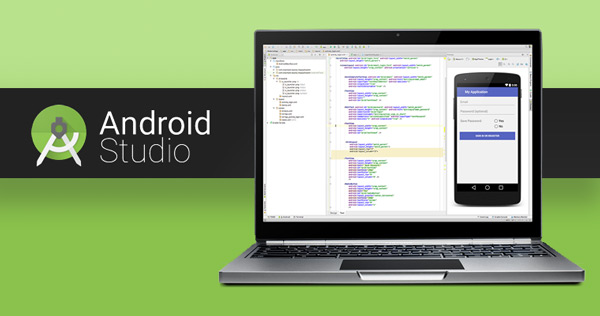
\includegraphics[width=0.6\linewidth]{androidstudio}
    \caption{Android Studio, un IDE flexible e intuitivo.}
    \label{fig:androidstudio}
\end{figure}

\subsection{LaTex}

LaTeX \cite{URL::LaTeX} es un sistema de composición de textos, orientado a la creación de documentos que presenten una alta calidad tipográfica. Por sus características y posibilidades, es usado especialmente en la generación de artículos y publicaciones científicas que incluyen, entre otros elementos, expresiones matemáticas, gráficos o figuras.

LaTeX está formado por un gran conjunto de macros de TeX, escrito por Leslie Lamport en 1984, con la intención de facilitar el uso del lenguaje de composición tipográfica, creado por Donald Knuth. LaTeX es software libre bajo licencia LPPL.

Se ha decidido usar esta herramienta debido a la calidad profesional de los documentos que es posible generar con ella. 
Otra de las ventajas de LaTeX es que permite separar el formato y el contenido del documento, lo cual permite concentrar el esfuerzo en la creación del contenido sin tener que ocuparse del diseño. 

\vskip 0.5in

\subsection{Github}

GitHub \cite{URL::Github} es una plataforma de desarrollo colaborativo para alojar proyectos que utiliza el sistema de control de versiones Git. 
GitHub fue escrito en Ruby on Rails. 
El código se almacena de forma pública, aunque también se puede hacer de forma privada, creando una cuenta de pago.

Se ha decidido crear un repositorio \cite{URL::repositorioAplicacion} en esta plataforma para poder llevar un control y una trazabilidad del proyecto \ULLAR{}. 
El tutor y el alumno han trabajado en este repositorio de manera conjunta. 
En el caso del tutor, principalmente para revisar el seguimiento semanal y llevar un control de las tareas. 
En el caso del alumno, para tener un repositorio donde subir los distintos elementos que se han ido generando a lo largo del trabajo. 
% Aparte de este repositorio, también se ha abierto un segundo repositorio \cite{URL::repositorioAplicacion} asociado a la oficina del software libre (OSL) para subir el código una vez terminado como parte del programa de apoyo a trabajos finales libres (PATFL) \cite{URL::PATFL} de la ULL.
En el repositorio del proyecto \cite{URL::repositorioAplicacion} están disponibles públicamente todos los ficheros necesarios para la elaboración con LaTeX de esta memoria, 
los ficheros correspondientes a la
presentación para la defensa de este TFG así como el proyecto de Android Studio que contiene el código fuente de \ULLAR{}. 

Mediante el uso de este repositorio, el alumno ha conseguido ampliar sus conocimientos en Git y familiarizarse con la interfaz de GitHub.

Para instalar GitHub en Linux se utiliza el siguiente comando:
\begin{lstlisting}
    sudo apt install git-all
\end{lstlisting}

\subsection{Guía de uso de estas tecnologías en relación con el proyecto \ULLAR{}}
En este apartado XXX se explica con cierto nivel de detalle los pasos a seguir para:
\begin{itemize}
\item Descargar desde su repositorio todo el código fuente, tanto de esta memoria como de la aplicación \ULLAR{}.
\item Compilar en Android Studio el proyecto \ULLAR{} para generar una aplicación para dispositivos móviles.
\item Compilar con Latex esta memoria para generar el corresponidente fichero en formato PDF.
\end{itemize}

\subsubsection{Descargar repositorio de la aplicación}

Para descargar el repositorio de \ULLAR{} se necesitará tener instalado en el ordenador el control de versiones de GitHub. Con GitHub ya instalado, se ejecuta el siguiente comando en consola para descargar el repositorio:

\begin{lstlisting}
    git clone https://github.com/alehdezp/TFG-ULL-AR 
\end{lstlisting}

En el caso de que no se tenga GitHub se puede descargar directamente desde el repositorio \cite{URL::repositorioAplicacion}, seleccionando el bóton ``Clone or download'' y luego se selecciona ``Download as ZIP''. Tras esto se descargará un archivo comprimido con todo el repositorio de \ULLAR{}.


\subsubsection{Compilar el proyecto en Android Studio}

Para compilar el proyecto es necesario tener instalado el IDE de Android Studio en el ordenador que se desee compilar el proyecto.

Una vez iniciado Android Studio, se selecciona que se quiere abrir un proyecto y se busca en la carpeta en la que se encuentra el repositorio de \ULLAR{} y se abre el proyecto que se encuentra en la ruta \textit{``app/ULL\_Navigation''}. 

La primera vez que se abre el proyecto, en el caso de que no se halla hecho automaticamente, se tiene  que seleccionar en la barra superior la opción de ``Build'' y luego ``Make Project''. Esto creára y configurar el proyecto para que se pueda empezar a trabajar con él.

Para poder instalar la aplicación que genera el proyecto en un dispositivo Android hay dos opciones. La primera es generar el un archivo ``.apk'', para generar este archivo se tiene que seleccionar en la barra superior la opción de ``Build'', luego ``Build Bundle(s) / APK(s)'' y por último ``Build APK''. Esto generará un fichero \texttt{app-debug.apk} en la ruta \textit{``ULL\_Navigation/app/build/outputs/apk/debug''}, este fichero hay que colocarlo dentro del dispositvo Android en el que se quiera instalar la aplicación y se ejecuta.

La seguna opción es ejecutar e instalar directamente la aplicación desde Android Studio. Para ello hay que tener activado en el dispositivo Android la opción de depuración por USB. Esta opción solo estará disponible cuando se tenga activado el modo desarrollador en el dispositivo Android, en función de la marcar y modelo del dispositivo la forma en la que se activa este modo varía. Con la opción activada solo hay que conectar el dispositivo al ordenador y seleccionar en el móvil el modo de ``Transeferencia de archivos'', a continuación en Android Studio se selecciona la opción de ``Run'' y luego ``Run 'app'''. Con estos pasos ya instalará la aplicación en el dispositivo y se pediran permisos en el dispositivo móvil para confiar en el desarrollador e instalar la aplicación \ULLAR{}. 


\subsubsection{Compilar la memoria del proyecto}

Para compilar el proyecto en LaTeX en un máquina con Linux es necesario instalar ``TeX Live'' y ``make''. Con el siguiente comando se instalarán ambos:
\begin{lstlisting}
    sudo apt install texlive-full make 
\end{lstlisting}

Dentro de la carpeta \textit{``Memoria/''} del repositorio, se abrirá una consola y se ejecutará el siguiente comando el cual genera el archivo con la presente memoria \texttt{memoria-TFG-Alejandro.pdf}.


\section{Tecnologías utilizadas}

A continuación, se revisan las distintas tecnologías utilizadas en el desarrollo de la aplicación.

\subsection{El Sistema Operativo Android}

Android \cite{URL::Android} es un sistema operativo (SO) que emplea Linux en la interfaz del hardware.  Los componentes del SO subyacentes se codifican en C o C++, pero las aplicaciones se desarrollan en Java. De esta manera Android asegura una amplia operatividad en una gran variedad de dispositivos debido a dos hechos: la interfaz en Linux ofrece gran potencia y funcionalidad para aprovechar el hardware, mientras que el desarrollo de las aplicaciones en Java permite que Android sea accesible para un gran número de programadores conocedores del código.

Este SO fue diseñado principalmente para dispositivos móviles con pantalla táctil: dispositivos móviles, tablets y otros dispositivos como televisores o automóviles. Fue desarrollado inicialmente por Android Inc., empresa que fue respaldada económicamente por Google y más tarde adquirida por esta misma empresa.

% Actualmente tiene una gran comunidad de desarrolladores creando aplicaciones para extender la funcionalidad de los dispositivos. A fecha de hoy existen más de un millón de aplicaciones disponibles para la tienda oficial de Apps de Android, Google Play \cite{URL::GooglePlay} sin tener en cuenta las aplicaciones de otras tiendas no oficiales, como, por ejemplo, la tienda de aplicaciones de Samsung Apps \cite{URL::SamsungApps}. 

\subsection{Realidad Aumentada}

La Realidad Aumentada (RA) \cite{URL::RealidadAumentada} o Augmented Reality (AR) en inglés, es el término que se usa para definir la visión de un entorno físico del mundo real, a través de un dispositivo tecnológico. Este dispositivo, permite expandir el mundo físico añadiendo capas de información digital generadas por un computador, como pueden ser imágenes, sonidos y vídeos a la visión del entorno en tiempo real. 

La RA está cambiando la manera en la que sus usuarios pueden ver el mundo. Actualmente es una tecnología que se encuentra en auge debido a su enorme potencial. Empresas de numerosos sectores ya han estado invirtiendo en su desarrollo debido a que los beneficios que traerá esta tecnología y las posibles aplicaciones por descubrir son prometedoras.


En un futuro la RA estará integrada en el día a día y formará parte de la vida cotidiana. Sus posibles aplicaciones no tienen límites, pueden llegar desde reconocer plantas e incluso monumentos y mostrar información sobre lo que se está viendo, hasta añadir información en tiempo real en una operación a un paciente, comprobar cómo queda un mueble en un salón o sus aplicaciones para realizar videojuegos, como se puede comprobar con el reciente éxito de Pokemón Go!. 

\begin{figure}[h]
    \centering
    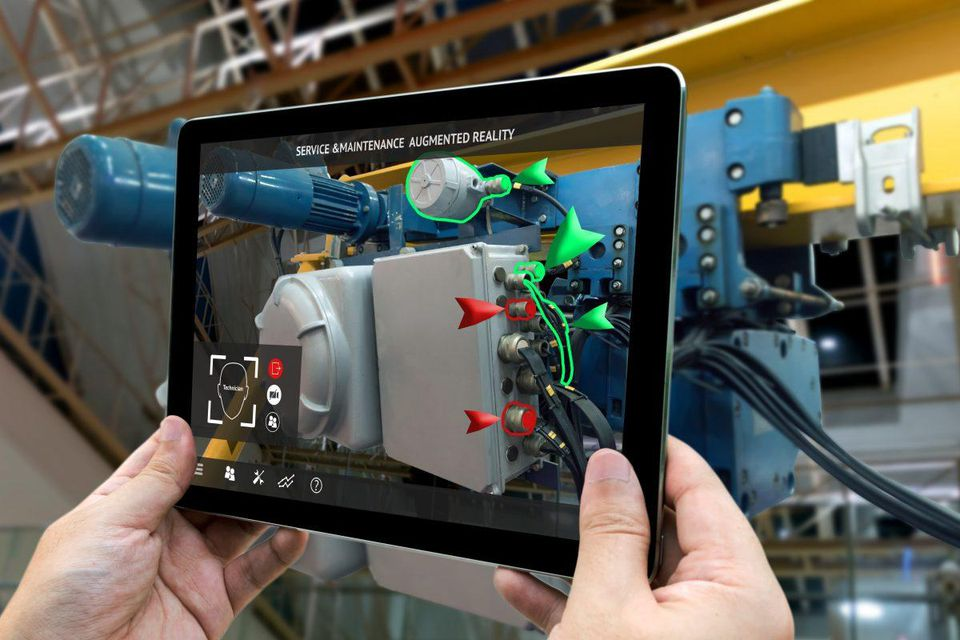
\includegraphics[width=0.6\linewidth]{imagenRAMantenimiento}
    \caption{Ejemplo de uso de la RA en servicios de mantenimiento.}
    \label{fig:googleglass}
\end{figure}

A continuación, se explicará en detalle:
\begin{itemize}
\item ¿Cómo funciona esta tecnología?.
\item Tipos de Realidad Aumentada.
\item Diferencias entre Realidad Aumentada y Realidad Virtual.
\item Realidad Mixta.
\item Futuro y usos de la Realidad Aumentada.
\item Integración de Realidad Aumentada en Android Studio.
\end{itemize}  

\subsubsection{¿Cómo funciona esta tecnología?}
La RA necesita de un dispositivo de visualización en el que mostrar esta unión del entorno real junto con la información digital. Esta unión puede ser visualizado en múltiples dispositivos: pantallas, gafas, dispositivos portátiles, dispositivos móviles, etc.
 
Además de estos sistemas de visualización, se necesita de un sistema de computación que realice los cálculos y reciba los datos provenientes de múltiples sensores, es decir: una CPU, una GPU, RAM, GPS, WIFI, bluetooth, acelerómetro, giroscopio, cámara, etc. Gracias a estos elementos el sistema puede reconocer el entorno real.

Todo esto necesita una parte software. El software en una primera parte deberá de reconocer el terreno, ubicaciones, objetos e imágenes, mediante los datos de los sensores y la cámara. Este proceso de transformación de diferentes conjuntos de datos a un sistema de coordenadas se llama registro de la imagen \cite{URL::ImageRegister}. 

Posteriormente el software deberá reestructurar el mundo real en función del registro de imágenes, añadiendo y combinando la información correspondiente al entorno para generar la imagen de RA. Existen múltiples maneras en las que se puede reestructurar este mundo. 

\begin{figure}[h]
    \centering
    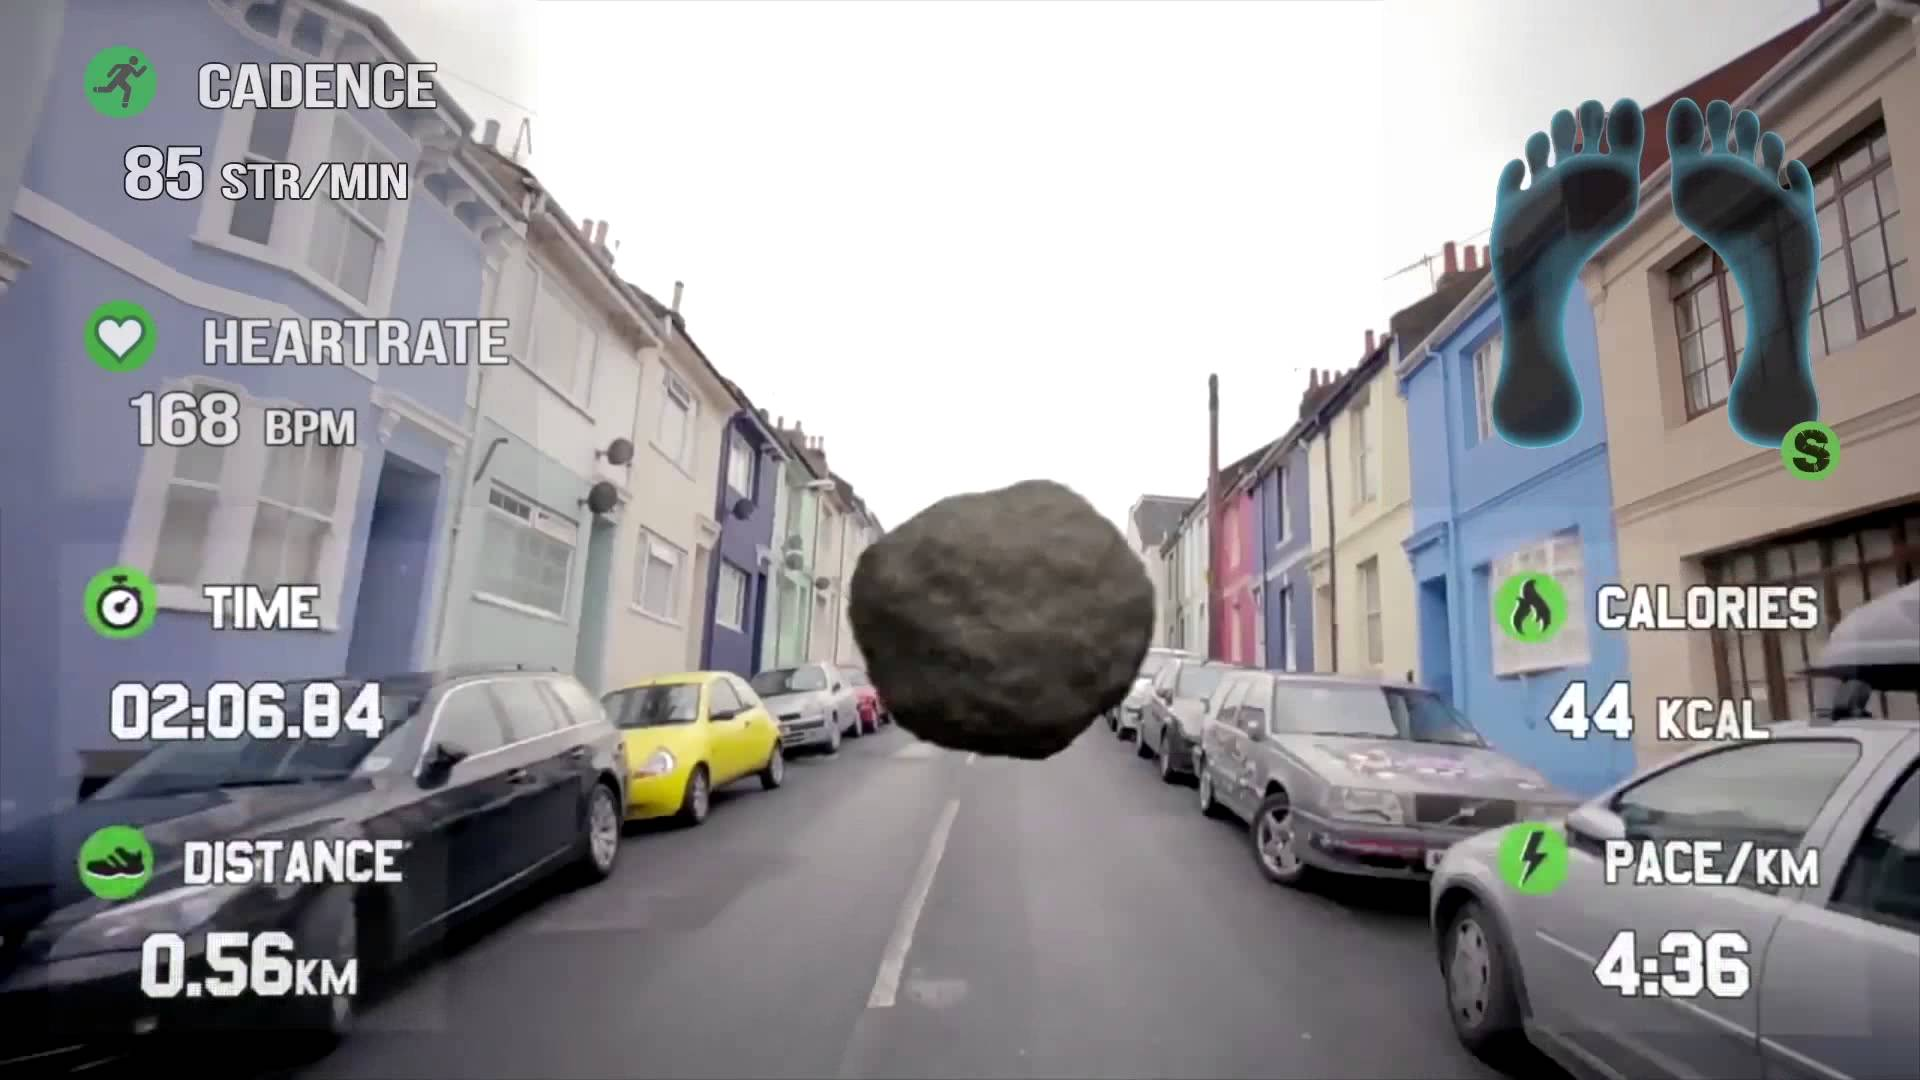
\includegraphics[width=0.6\linewidth]{googleglass}
    \caption{Google Glass. Desmostración del uso de RA en deportes.}
    \label{fig:googleglass}
\end{figure}

\subsubsection{Tipos de Realidad Aumentada}

Existen hoy en día cuatro tipos de RA:

\begin{itemize}
    \item 
    Marker-based AR. Se basa en el reconocimiento de imágenes conocidas como \textit{marker} o marcadores. 
		Los marcadores son imágenes distintivas que son reconocidas fácilmente por un dispositivo, debido a que contienen puntos visuales únicos. Un buen ejemplo de este tipo de imágenes son los conocidos códigos QR \cite{URL::CodigoQR}. Una vez se ha reconocido un marcador, se puede agregar información virtual. Esta información puede ser la incorporación de animaciones o vídeos en una página de un libro de texto, simulaciones de objetos 3D o arquitecturas sin llegar a construirlas de forma física (véase Figura \ref{fig:markerAR}).
    \begin{figure}[h]
        \centering
        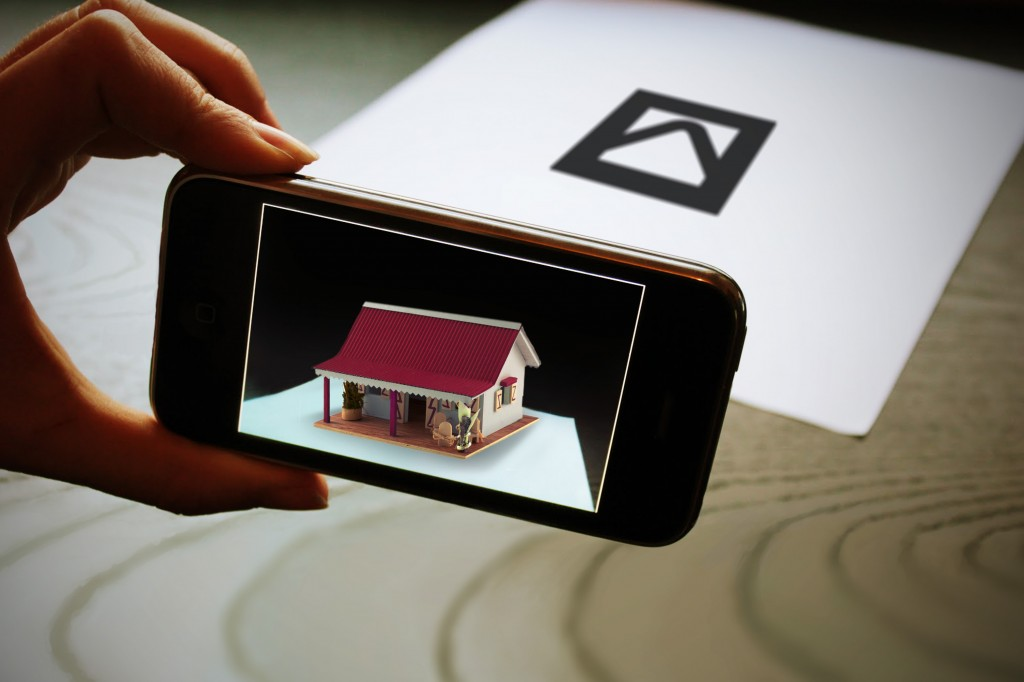
\includegraphics[width=0.6\linewidth]{marker-ar}
        \caption{Marker-bases AR. Demostración de su funcionamiento.}
        \label{fig:markerAR}
    \end{figure}

   

    \item Markerless AR. Corresponde a la RA que recoge los datos de su posición y orientación para mostrar la información correspondiente a esa área. Estos sistemas utilizan los datos obtenidos de la cámara, GPS, brújula, giroscopio y acelerómetro para establecer la ubicación del usuario en el entorno. Utiliza técnicas para reconocer terreno o ambientes para calcular la posición y orientación de la cámara. Con este tipo de tecnología se puede probar un mueble en el salón antes de llegar a comprarlo.

 
    \item Pojection-based AR. Este modo de RA consiste en la proyección de luz en superficies y objetos en el mundo real. Existen muchos usos interesantes de esta tecnología, como aplicaciones para el uso de teclados virtuales proyectados que reconozcan cuando una ``tecla" es pulsada. Esta proyección también se puede hacer en medio del aire con ayuda de la tecnología de láseres de plasma.

    \item Superimposition-based AR. Esta tecnología reemplaza la imagen original por una de RA, de forma completa o parcial. El reconocimiento de objetos juega un papel fundamental en este tipo de tecnología. Tiene gran utilidad el campo de la medicina, por ejemplo, un doctor podría examinar a un paciente mientras ve la imagen de RA que se creado a partir de una visión de rayos X y la imagen real de paciente, así puede ver y entender mejor el daño en un hueso.
\end{itemize} 

Aparte de los cuatro tipos de RA, existen subtipos dentro de cada uno de ellos.

``Location-based AR" es un tipo de ``Markerless AR"  que se centra más en los cálculos de la orientación y geolocalización del dispositivo. Esta técnica RA puede proveer de ayuda viajeros que necesiten una mano para moverse por la ciudad, ya que mediante el reconocimiento de su ubicación y la orientación pueden mostrarles la ruta para llegar a su destino o mostrarle información de los puntos de interés que les rodean. Esta será la técnica de RA implementada en la aplicación a desarrollar en este TFG. 


\subsubsection{Diferencias entre Realidad Aumentada y Realidad Virtual}
En los últimos años la realidad virtual (RV) \cite{URL::VR} o virtual reality (VR) en inglés y la realidad aumentada han empezado a recibir mucha más atención. Llevando a desarrolladores realizar integraciones de ambas tecnologías en numerosas industrias.

De acuerdo con un análisis de expertos, la RV iba tener el liderazgo en 2018 como tecnología pionera, sin embargo, la RA va a tener mucha más importancia y a largo plazo, llegará a formar parte del día a día.

La realidad virtual es un entorno de escenas u objetos de apariencia real. Aleja al usuario del entorno real y le brinda la sensación de estar inmerso en él. Dicho entorno es contemplado por el usuario a través de un dispositivo conocido como gafas o casco de realidad virtual. Este puede ir acompañado de otros dispositivos, como guantes o trajes especiales, que permiten una mayor interacción con el entorno, así como la percepción de diferentes estímulos que intensifican la sensación de realidad.

La realidad aumentada no aísla al usuario de mundo exterior, sino que traslada al mundo real objetos virtuales mediante la superposición de imágenes en tiempo real. 

\subsubsection{Realidad Mixta}

Existe otro tipo de tecnología que nace de la unión de realidad aumentada y la realidad virtual, la realidad mixta (RM) \cite{URL::RM}. Es un tipo de realidad similar a la realidad aumentada, pero con una idea más ambiciosa de mezclar lo real con lo virtual.

\begin{figure}[h]
    \centering
    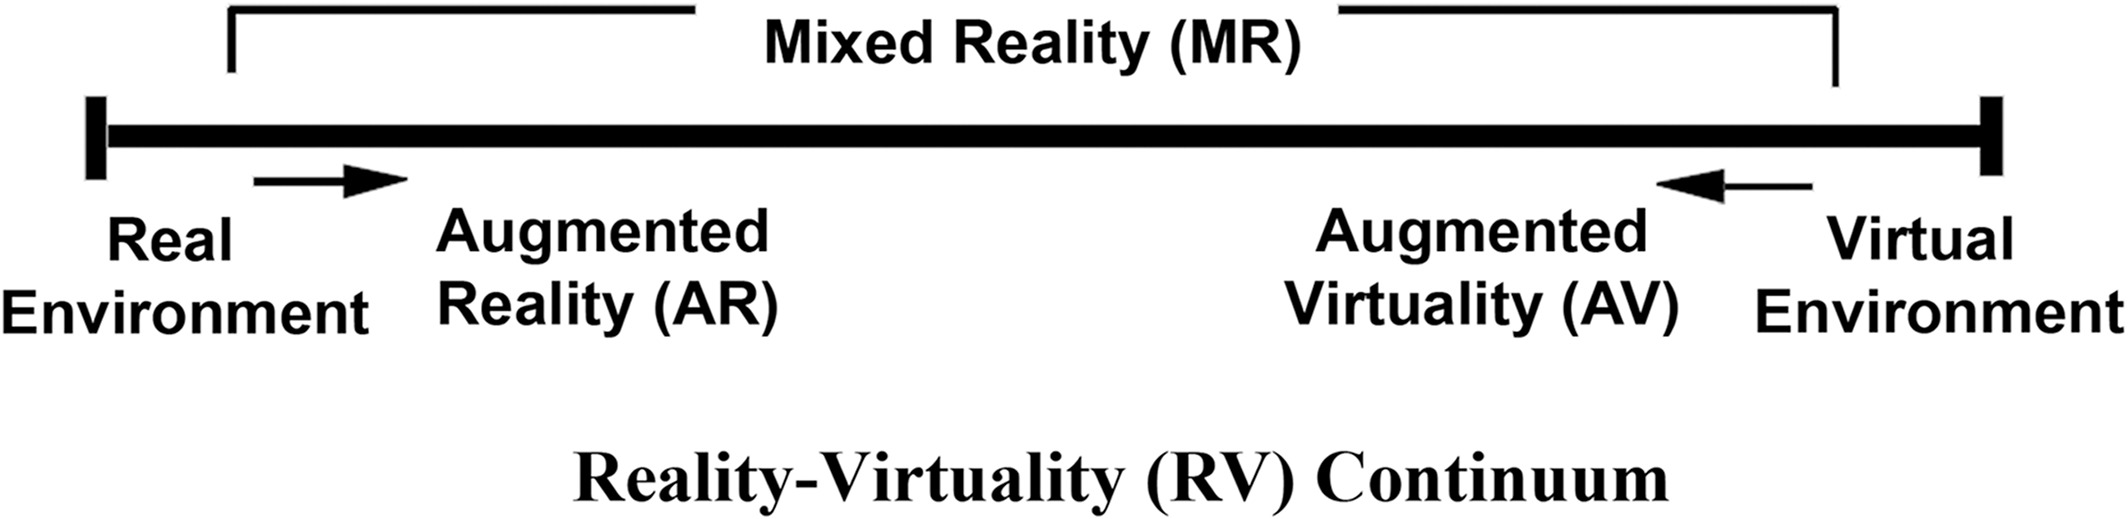
\includegraphics[width=0.6\linewidth]{realidamixta}
    \caption{ Espacio de la Realidad Mixta. }
    \label{fig:realidadMixta}
\end{figure}

En la RM se trata de llevar el mundo real al mundo virtual (véase Figura \ref{fig:realidadMixta}). La idea es generar un modelo 3D de la realidad y sobre él superponer información virtual. De esta forma, se podrán combinar ambas realidades para agregar contenido adicional de valor para el usuario de RM. La RM es mucho más inmersiva que la realidad aumentada y requiere de mucha más capacidad de procesamiento. 

\subsubsection{Futuro y usos de la Realidad Aumentada}
Actualmente la RA se encuentra más disponible a cualquier usuario, que en años anteriores. 
Dispositivos como los teléfonos móviles ya incorporan las primeras muestras de esta tecnología, la cual está aún en una fase inicial de desarrollo, pero ya se puede ver el potencial y la enorme importancia 
que va a cobrar en un futuro.

Los usos actuales de esta tecnología se acercan a todos los sectores conocidos:

\begin{itemize}
    \item Realidad Aumentada en educación. La llegada de la RA afectará a los procesos convencionales de aprendizaje. La RA tiene la capacidad de cambiar el horario y el lugar en el que se estudia y la posibilidad de introducir nuevos métodos de enseñanza. 
    
Actualmente gran parte de la población joven tiene un dispositivos móvil el cual es un medio idoneo para la RA. 
Por lo tanto, se dan unas condiciones adecuadas para que la RA profundice en el campo de la educación y se hagan más descubrimientos ya que cada estudiante va a tener un dispositivo a mano capaz de reproducir la RA, 
lo cual puede ayudar al alumnado a tener contenidos más accesibles sobre cualquier asignatura o conseguir que información compleja sea más fácil de entender. Un ejemplo claro sería la creación de libros interactivos que al ser apuntados con la cámara del móvil muestren el funcionamiento en 3D de un volcán (véase Figura \ref{fig:education-example}) o del latido de un corazón.

    \begin{figure}[h]
        \centering
        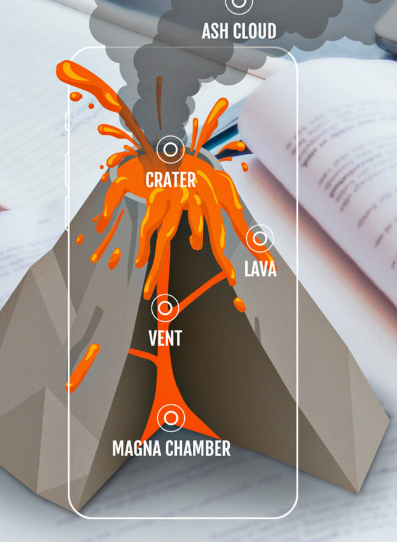
\includegraphics[width=0.35\linewidth]{education-example}
        \caption{RA Volcán. Ejemplo de uso de RA en Educación. }
        \label{fig:education-example}
    \end{figure}
    
    \item Realidad Aumentada en los videojuegos. Sin duda uno de los sectores en lo que más interés se tiene para desarrollar esta tecnología y quizás donde más se haya avanzado en realidad aumentada. Todas las grandes empresas de este sector tienen ya potentes desarrollos y lanzamientos de videojuegos que combinan la realidad física con la virtual, con múltiples posibilidades de personalización dentro de cada juego. En un futuro esta tecnología revolucionará todo el sector de los videojuegos y cambiará la manera en la que se interactúa con ellos.   
    
    Un claro ejemplo del potencial de la RA en este sector, está en el éxito de Pokemón Go! \cite{URL::Pokemon-Go}. Una aplicación para dispositivos móviles que utiliza técnicas de RA basadas en la localización, la cual a través de la cámara del dispositivo y modelos 3D para representar a los personajes de la saga Pokemón \cite{URL::Pokemon}, los cuales se encuentran escondidos en ubicaciones del mundo real.  
    
    
    
    \item Realidad Aumentada en la industria. El desarrollo de aplicaciones de RA en el ámbito industrial también está creciendo, ya que ayuda a mejorar la productividad de los ciclos de trabajo. Por ejemplo, algunas empresas están desarrollando aplicaciones que ayuden a los trabajadores de una cadena de montaje. De este modo, los empleados pueden obtener información adicional sobre las acciones que llevan a cabo. Este mismo sistema también se puede implementar en las reparaciones de vehículos o maquinaria industrial, ya que la aplicación puede mostrar toda clase de avisos sobre las piezas deterioradas. Incluso puede llegar a mostrar contenido visual en 3D sobre cómo llevar a cabo la reparación o sustitución de esos elementos. 
    

    \item Realidad Aumentada en turismo. El negocio turístico siempre ha intentado estar al día con la nueva tecnología para poder ofrecer nuevos servicios, formas de publicitarse, transporte y actividades de ocio. Por eso no es raro que la RA se haya hecho un hueco en este sector debido al potencial que tiene para mejorar la experiencia de los turistas. 
    
    La RA tiene la capacidad de generar aplicaciones que permitan a los turistas realizar una visita guiada por las ciudadades que visiten, permitiéndoles moverse sin problemas por la ciudad, señalando puntos de interés, datos históricos, restaurantes, hoteles, etc. El mismo concepto podría aplicarse en museos y zoos. Otro uso interesante sería el de romper la barrera del lenguaje gracias a la traducción inmediata de señales, textos y anuncios, al idioma del turista. Para los Juegos Olímpicos de Tokio 2020 se espera tener esta tecnología preparada para poder traducir a los visitantes en tiempo real todos los textos, señales y anuncios, a través de sus dispositivos móviles.   

    

    \item Realidad Aumentada en medicina. En cuanto a la medicina, es interesante ver cómo avanza la tecnología en este campo que sin duda apunta prometedor para mejorar la calidad de vida y salud de la población.
    
    Los principales usos que se plantean se encuentran enfocados principalmente en los quirófanos, en los que el especialista o cirujano monte una especie gafas-pantalla que le permitan realizar la operación sin la necesidad de apartar la vista del paciente para consultar información o ir monitorizando la operación. Esto se traduce en operaciones más rápidas y seguras sin que el cirujano se despiste. A su vez, esto podría mostrar información anatómica sobre el paciente en tiempo real, es decir, gracias a algoritmos de inteligencia artificial, permitir identificar nervios, venas mayores y huesos, y que estos sean marcados con un distinto color, facilitando mucho las labores de los médicos.

\end{itemize}

\subsubsection{Android Studio y la RA}


Para la integracion de realidad aumentada en Android, se han probado y estudiado los kits de desarrollo de software (SDK \cite{URL::SDK}) de realidad aumentada disponibles para Android Studio. Los SDK que han sido evaluados son:



\begin{itemize}
    
    \item  \textbf{Vuforia} \cite{URL::vuforia} es un SDK de realidad aumentada que permite a los desarrolladores de aplicaciones crear rápidamente experiencias de RA inmersivas, de alta fidelidad y centradas en el móvil. El SDK de Vuforia aprovecha la tecnología de visión por computadora para identificar y rastrear imagenes y objetos 3D en tiempo real. Esta funcionalidad permite orientar y colocar objetos virtuales, incluidos modelos 3D y otros contenidos, en relación con el entorno del mundo real. Los modelos 3D y la información digital se pueden superponer sobre la escena del mundo real y verlos en relación con el entorno a través de un dispositivo móvil.
    
Este SDK es uno de los mejores del mercado con buen soporte para aplicaciones multiplataforma. 
Un inconveniente de Vuforia es que está diseñado para desarrollar aplicaciones y juegos principalmente en plataformas como Unity \cite{URL::Unity}. 
En cuanto al SDK para Android Studio, la falta de soporte, de documentación y los númerosos problemas hallados a la hora de instalarlo, lo convierten en un SDK con el que nos ha sido muy difícil trabajar. 
Es por ello que se ha decidido descartar Vuforia para su integración en \ULLAR{}.

    \item \textbf{Kudan AR SDK} \cite{URL::kudan} es una plataforma diseñada para desarrolladores de RA como una plataforma preprada para admitir tanto en el reconocimiento basado en marcadores como sin marcadores y el seguimiento de de los mismos. 
El motor Kudan SDK principal, se desarrolla completamente en C++ y posee optimizaciones específicas de la arquitectura desarrolladas para proporcionar un rendimiento más rápido y sólido sin afectar negativamente el espacio de memoria. 
    
La instalación de Kudan AR fue rápida y sencilla, debido a que Kudan dispone de la documentación necesaria para instalarlo en Android Studio. 
Además, dispone de una guía bien explicada para comenzar la implementación de sus funcionalidades. 
Se ha optado por la integración de este SDK debido a su sencillez y a que ofrece los requisitos mínimos para el objetivo de RA de \ULLAR{}.

\item  \textbf{MaxST SDK} \cite{URL::maxst} de realidad aumentada proporciona un motor RA integral multiplataforma equipado con todas las características requeridas por los desarrolladores para crear experiencias y aplicaciones de RA. 
MaxST AR proporciona las siguientes funcionalidades: seguimiento instantáneo, SLAM \cite{URL::SLAM} (utiliza la cámara del teléfono inteligente para crear un ``mapa virtual'' del área circundante), rastreo de objetos y reconocimiento de imágenes y de marcadores.
    
MaxST AR ofrece unos de los mejores soportes para la integración de un SDK de RA en Android Studio. 
Dispone de  tutoriales en su página web para la instalación del SDK, explicando el funcionamiento e implementación de cada una de las funcionalidades que ofrece. 
No se le ha encontrado ningún inconveniente para integrarlo en la aplicación, pero se ha preferido integrar Kudan AR SDK por su simplicidad.
\end{itemize}

% Se ha optado por utilizar ``Kudan AR SDK" para el desarrollo de la aplicación de este TFG debido a problemas de compilación y flexibilidad en las opciones gratuitas de los otros dos SDK en Android Studio.  


\subsection{Node.js}

Node.js \cite{URL::Nodejs} es una librería y entorno de ejecución de E/S dirigida por eventos y por lo tanto asíncrona que se ejecuta sobre el intérprete de JavaScript creado por Google llamado Chrome V8 \cite{URL::ChromeV8}. Node.js es un entorno de JavaScript del lado del servidor \cite{URL::serverside}, basado en eventos. Utilizar el motor de Chrome V8 permite a Node.js un entorno de ejecución que compila y ejecuta JavaScript a velocidades increíbles.

Node.js fue desarrollado con el objetivo que fuera un sistema escalable y que tuviera la consistencia de generar un elevado número de conexiones de forma simultánea con el servidor. La mayoría de las tecnologías que de los servidores tradicionales tienden a accionar las peticiones de forma aislada y mediante hilos independientes. Esto se traduce en que a mayor número de solicitudes mayor es la cantidad de recursos necesarios para responderlas. Node.js se ha desarrollado para optimizar la gestión de estas solicitudes.

La solución que propone Node.js se basa en el tratamiento de las solicitudes de forma unificada en un único hilo complementado con un bucle de eventos de tipo asíncrono. De este modo cada petición que se recibe se trata como un evento y pertenecen a este único bucle (véase Figura \ref{fig:nodejsEx}). Este nuevo replanteamiento proporciona un lenguaje con una capacidad para gestionar una gran cantidad de solicitudes y conexiones con la máxima eficiencia.

Node.js utiliza un E/S de tipo asíncrono. En los modelos de tipo asíncronos, las tareas que efectúa el servidor se realizan de manera simultánea y repartidas entre los hilos del procesador. Este procedimiento evita que se produzcan bloqueos y proporciona una mayor potencia y velocidad de procesamiento.

     
\begin{figure}[h]
    \centering
    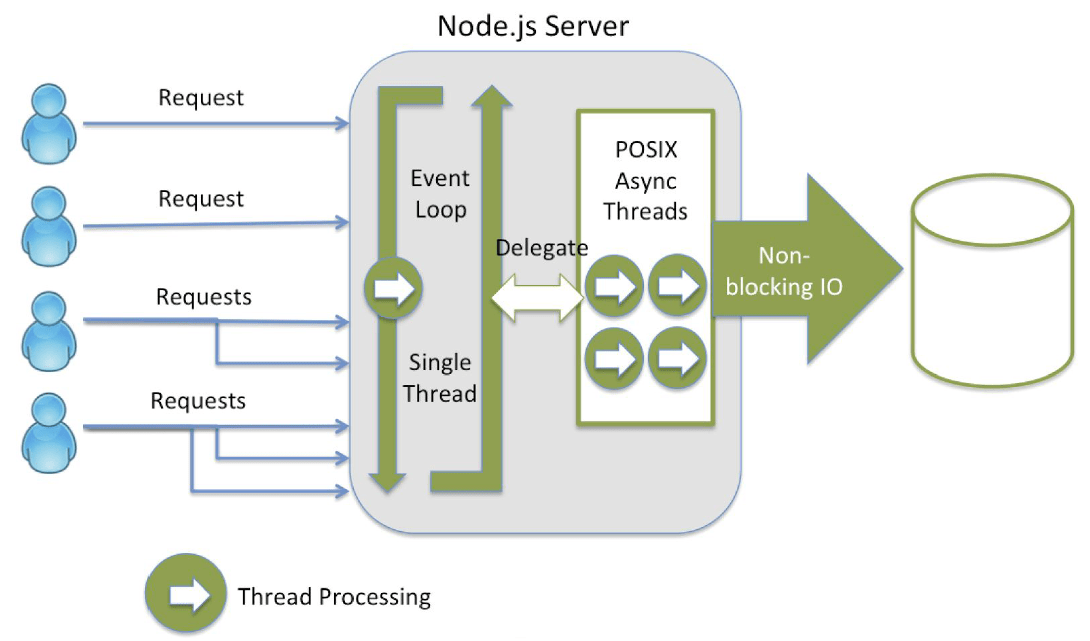
\includegraphics[width=100mm,scale=1]{nodejsEx}
    \caption{Funcionamiento de Node.js.}
    \label{fig:nodejsEx}
\end{figure}


% Para poder comunicarse con diferentes clientes el servidor se encarga de unas tareas denominadas E/S, las cuales hacen referencia a aquellas que están destinadas una entrada y salida de información. Un E/S de tipo sincrónica lo cuales se ejecutan las instrucciones de forma lineal, es decir una instrucción no se ejecuta hasta que la anterior no ha terminado de ejecutarse. Esto llevaba a el alargamiento innecesarios de algunos procesos de trabajo y a la tendencia de que se produzcan bloqueos. 

% JavaScript es un lenguaje cuyo principal uso se centra en el lado del cliente. Sin embargo Node.js está diseñado para ejecutar JavaScript desde lado del servidor. JavaScript es un lenguaje muy extendido entre los desarrolladores lo cual hace que Node.js sea una alternativa más sencilla. Pero esta no es la única razón por la que se eligió este lenguaje. Sus rasgos de lenguaje asíncrono y orientado al diseño de eventos ofrecían mejores condiciones para trabajar con él en esta arquitectura.   

Otro de sus puntos fuertes es su gestor de paquetes Node Package Manager  (NPM). Gracias a este gestor se pueden instalar paquetes, módulos y agregar dependencias de manera simple.

Se ha optado por el uso de un servidor que implemente la tecnología Node.js como servidor de \ULLAR{} por la facilidad  para ejecutar este servidor en cualquier tipo de sistema operativo y para su futura integración en la nube, 
gracias a la plataforma Heroku de la que se hablará más adelante. 
Otra de las razones por las que se ha elegido Node.js es porque el proceso de desarrollo y programación es rápido y sencillo y además se tenían conocimientos previos sobre esta tecnología, lo que ha facilitado su uso.


\begin{figure}[h]
\centering
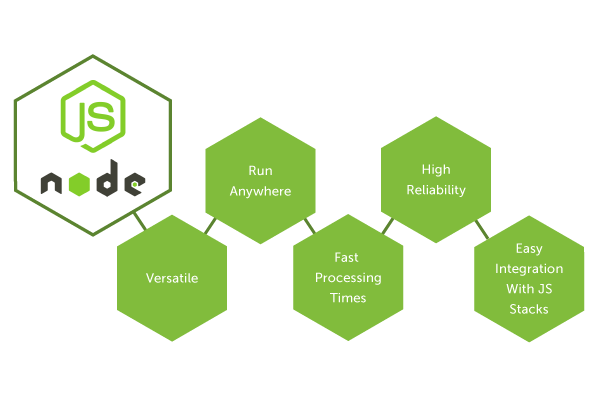
\includegraphics[width=115mm,scale=1]{nodejsfunc}
\caption{Ventajas de Node.js.}
\label{fig:nodejsVentajas}
\end{figure}

% \subsubsection{¿Porqué Node.js?}
% \begin{itemize}
%     \item Fácil de integrar e instalar en cualquier servidor, sin importar el sistema operativo.
%     \item JavaScript como base. Un lenguaje conocido por cualquier programador.
%     \item Gran rendimiento, permite generar a su vez arquitecturas potentes y sólidas.
%     \item Su alta capacidad de escalabilidad. La creación de aplicaciones web con la capacidad de atender muchos miles de solicitudes en un único servidor de forma simultánea, sin la necesidad de tener que incrementar las infraestructuras de servidores.
%     \item Un proceso de desarrollo y programación de aplicaciones rápido y liviano.
% \end{itemize}


Para instalar Node.js en una máquina con Linux se deben ejecutar estos comandos:
\begin{lstlisting}
    $ curl -sL https://deb.nodesource.com/setup_11.x | sudo -E bash -
    $ sudo apt install -y nodejs
\end{lstlisting}


% \subsubsection{ Desventajas }

% \begin{itemize}
%   \item Se desconoce el funcionamiento e implementación de Node.js en empresas de hosting.
%   \item La API es inestable en lo que respecta al cambio entre versiones.
%   \item Falta de Librerías en General. Dado que JavaScript no ha sido muy popular en el lado del servidor existe algunas librerías de las que carece en la actualidad.
%   \item Es bastante flexible en cuanto las formas en la que se puede programar. Pero esto genera bastantes problemas debido a la falta de organización en el código. 
% \end{itemize}

\subsection{MongoDB}

\subsubsection{ Descripción }

MongoDB  \cite{URL::MongoDB} es un sistema de base de datos multiplataforma NoSQL   \cite{URL::NoSQL} orientado a documentos. Esta base de datos es de esquema libre, es decir, al contrario que las bases de datos relacionales no utilizan una tabla fija para guardar la información.

Un registro en MongoDB es un documento, cuya estructura de datos se compone por el par campo y valor. Utilizan un formato para guardar estas estructuras que se llama BSON  \cite{URL::BSON} también llamada JSON \cite{URL::json} Binario. Este formato tiene una ventaja pese a que puede ocupar más espacio de lo que lo haría el formato JSON. BSON guarda de forma explícita las longitudes de los campos, los índices de los arrays, y demás información útil para el escaneo de datos y así agilizar las búsquedas en estos documentos.

Estos documentos, que a su vez incorporan una clave primaria como identificador, son la unidad básica de datos en MongoDB. Las colecciones en MongoDB contienen un conjunto de documentos y funciones equivalentes a las de las bases de datos relacionales.

Debido a los requisitos de la aplicación, el uso de una base de datos de MongoDB
permitía la creación de una base de datos de esquema libre, es decir, sin la preocupación de crear tablas de datos para almacenar la información, que permitía guardar de forma simple toda la información necesaria para 
el funcionamiento de la aplicación. 
Además, las consultas a esta base de datos se facilitan con el uso de un servidor Node.js, que ofrece un conjunto de librerias y paquetes preparados para realizar la comunicación con una base de datos de MongoDB.

% La consola de mongo es una interfaz interactiva de JavaScript la cual permite a los usuarios de MongoDB consultar, actualizar y administrar estas bases de datos. Esta consola es un componente estándar de las distribuciones de Open Source.

\begin{figure}[h]
    \centering
    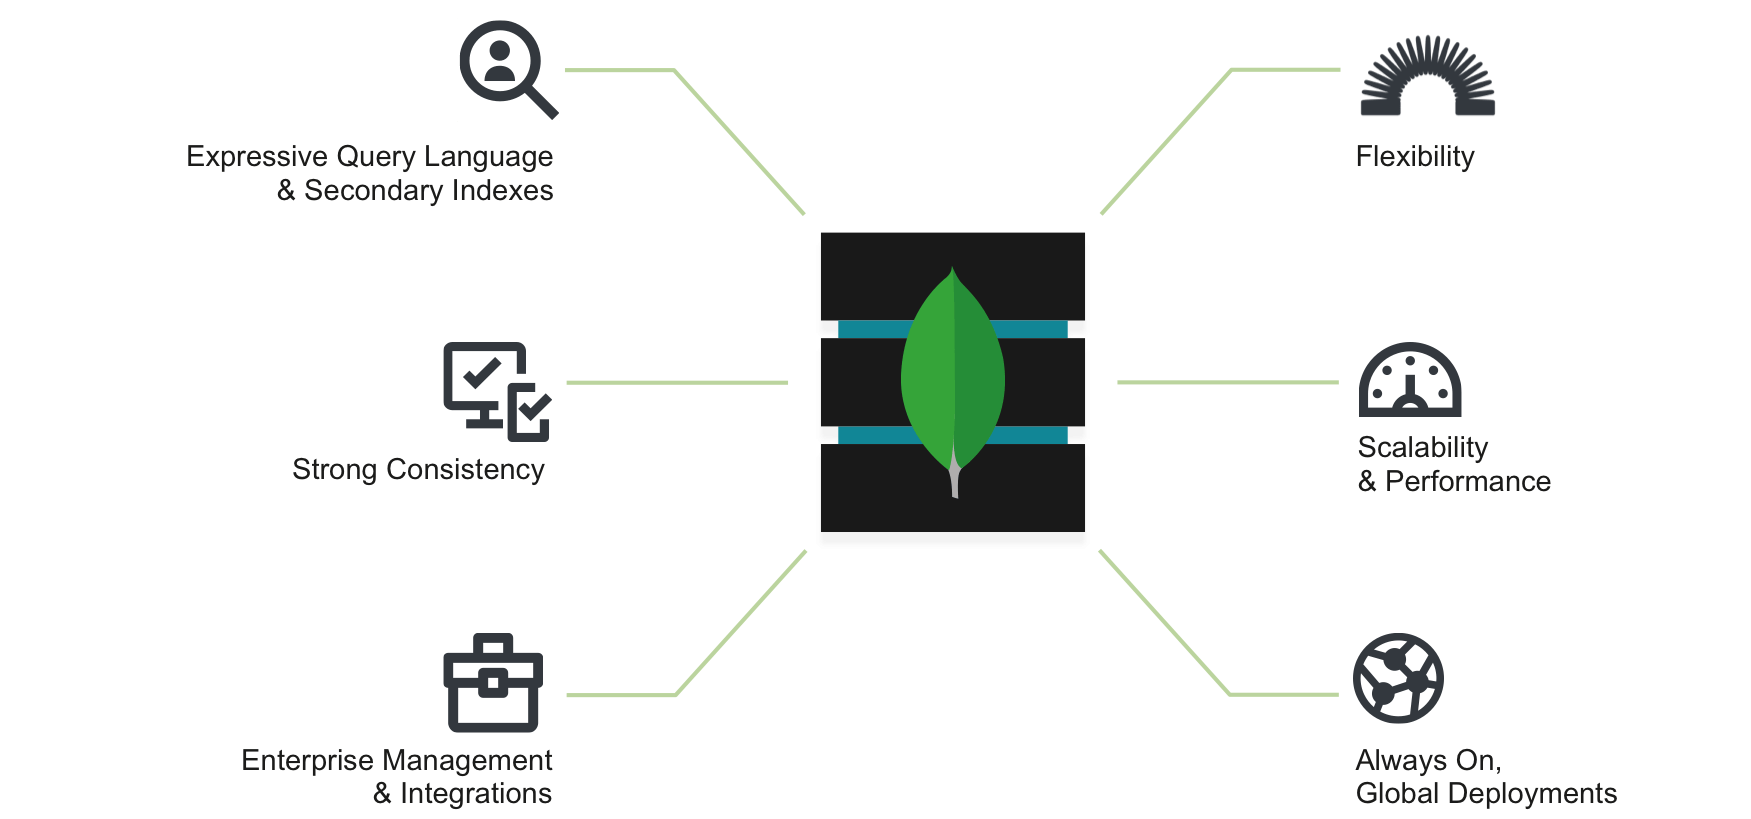
\includegraphics[width=150mm,scale=2]{mongodb-architecture}
    \caption{ Ventajas de MongodDB. }
    \label{fig:mongoDBarquitectura}
\end{figure}


% \subsubsection{ Ventajas de MongoDB }


% \begin{itemize}
    
%     \item El hecho de que sea una base de datos NoSQL, significa que no necesita esquemas predefinidos y puede guardar cualquier tipo de datos. Esto otorga una gran flexibilidad para crear cualquier tipo de campos que se necesiten en un documento, permitiendo mayor escalabilidad en MongoDB comparado a las bases de datos tradicionales.

%     \item A su vez, el uso de documentos para guardar la información hace que sea mucho más fácil de mapear estos datos en los lenguajes nativos de programación.

%     \item Es fácil  acceder a los documentos si se indexan. En MongoDB este indexado provee de rápidos tiempos de respuesta a las peticiones, esto le permite ser hasta 100 veces más rápido que los modelos de bases de datos relacionales.

%     \item MongoDB es una base de datos distribuida, por lo que es fácil de usar y proporciona una elevada disponibilidad, escalabilidad horizontal y distribución geográfica.
    
 
% \end{itemize}

% Por otro lado existen una serie de inconvenientes y limitaciones:

% \begin{itemize}
%   \item No soporta las consultas SQL ya existentes. Un ejemplo de esta es la consulta Join \cite{URL::JoinSQL}, la cual supone una desventaja en cuanto a rendimiento si se tienen que añadir manualmente los datos en el caso de querer realizar una consulta de este tipo.

%   \item No es una solución adecuada para aplicaciones con transacciones complejas.
%   \item Falta de estandarización entre las diferentes bases de datos NoSQL.
% \end{itemize}

\subsection{ Heroku }

Heroku es una plataforma como servicio de computación (PaaS \cite{URL::PaaS}) en la nube que soporta distintos lenguajes de programación. Heroku permite a desarrolladores y compañías construir, proporcionar, monitorizar y escalar aplicaciones. Es una forma sencilla de montar una infraestructura en la nube.

Heroku es conocida por ejecutar las aplicaciones en ``dynos". Un dyno es simplemente un ordenador virtual que pueden ser encendido y/o apagado en función del tamaño y requisitos de la aplicación.

A cada uno de estos dynos se le puede configurar más espacio o capacidad de procesamiento, o se pueden añadir más dynos si la aplicación lo necesita. Heroku a cada mes realiza un cobro en función de los dynos que el usuario tenga contratados. 

Se ha optado por utilizar el dyno gratis que ofrece Heroku a cada repositorio. El cual tienen un límite de 1000 horas activas al mes y se pone en suspensión a los 30 minutos sin recibir tráfico. Una vez que vuelve a recibir tráfico se activa de nuevo.   

Se ha utilizado Heroku para albergar el servidor de \ULLAR{}, ya que ofrece un servicio gratuito idóneo para el diseño de pequeñas aplicaciones web en la nube, sin la complejidad de estar implementando un servidor físico. 

Para instalar Heroku basta seguir las indicaciones que se hallan en \cite{URL::HerokuCLI}.


\subsection{ mLab }
mLab es un servicio de base de datos en la nube totalmente gestionado que ofrece aprovisionamiento y escalados automáticos de las bases de datos MongoDB, copia de seguridad y recuperación, monitoreo, herramientas de administración basadas en web y soporte experto. La plataforma de base de datos como servicio de mLab corre sus máquinas en proveedores de servicios en la nube como AWS \cite{URL::aws}, Azure \cite{URL::Azure} y Google Cloud \cite{URL::GoogleCloud}.

En esta plataforma se ubicará la base de datos de \ULLAR{}. 
Dadas las facilidades de acceso a ella e integración con el servidor de la aplicación en Node.js, es una opción simple, fácil de manejar y con posibilidad de escalar.

\subsection{ Google Maps }

La API de Google Maps \cite{URL::GoogleMapsApi} fue publicada para Android en 2008 y en 2012 para IOS. Esta API permite utilizar mapas basados en datos de Google Maps en una aplicación Android, y además ofrece métodos para personalizar el mapa:
\begin{itemize}
    \item Creación de marcadores, polígonos y superposiciones sobre el mapa para resaltar puntos o zonas. 
    \item Permite cambiar la vista del usuario de modo que se muestre un área del mapa en particular. 
    \item Ofrece la posibilidad de elegir el tipo de mapa: de carreteras, satélite, híbrido (fusión de carretera y satélite) y de terreno.
\end{itemize}

Esta API fácil de integrar y con soporte de Google, es la mejor opción para tener un mapa funcional y que permita ubicar al usuario de la aplicación.

%
% ---------------------------------------------------
%
% Proyecto de Final de Carrera:
% Author: Alejandro Hernández Padrón <alu0100703511@ull.edu.es>
% Capítulo: Objetivos 
% Fichero: Cap1_Goals.tex
%
% ----------------------------------------------------
%

\chapter{RA en entornos universitarios } \label{chap:RAEntornosUniversitarios}  

En este capítulo trataremos los usos y ventajas de la integración de la realidad aumentada en entornos universitarios.

La realidad aumentada se presenta en el ámbito educativo como una tecnología capaz de aportar transformaciones significativas en la forma en que el alumnado perciben y acceden a la realidad física, proporcionando así, experiencias de aprendizaje más ricas e inmersivas.

En la actualidad en educación, la realidad aumentada rara vez se usa, pero cada vez más docentes, investigadores y desarrolladores están comenzando a moverse hacia nuevos métodos de enseñanza más interactivos. Por ello, con la continua implantación de nuevas tecnologías en las aulas, junto al incremento de dispositivos móviles en la población, sitúa a la RA en una posición destacada para introducirse en las aulas. 

Las aplicaciones que tiene la RA, en lo referente a la creación de materiales didácticos y actividades de aprendizaje son múltiples, directas y fáciles de imaginar en prácticamente todas las disciplinas, sobre todo, las relacionadas con las ciencias aplicadas (ingeniería, química y física, biología), pero también en el campo del diseño industrial, la cirugía, la arqueología, etc.
La tecnología de la RA permite cambiar la forma de entender los contenidos de aprendizaje, puesto que aporta nuevas formas de interacción con el mundo real a través de capas digitales de información que amplían, completan y transforman en cierto modo la información inicial.

Los beneficios potenciales de la RA aplicados a la educación incluyen:
\begin{itemize}

    \item Aumentar o enriquecer la información de la realidad para hacerla más comprensible al alumno.
    
    % \item Permite múltiples formas de visualización de conceptos teóricos difíciles.

    \item El uso de una interfaz tangible para la manipulación de objetos, que permite observar un objeto desde diferentes puntos de vista,
    seleccionando, el alumno, el momento y posición de observación.

    \item Potenciar el aprendizaje ubicuo \cite{URL::AprendizajeUbicuo}.
    
    \item Crear escenarios “artificiales” seguros para el alumnado
    como pueden ser laboratorios o simuladores. 

    \item Enriquecer los materiales impresos para el alumnado con información adicional en diferentes soportes.
    
    \item Facilita la colaboración efectiva y discusión entre el alumnado.
    
\end{itemize}

Numerosos artículos han demostrado la eficacia de que las aplicaciones de RA pueden mejorar el proceso de aprendizaje, aumentar la motivación y la efectividad \cite{URL::animationeco} \cite{URL::ar2}. Pero hay que tener en cuenta una serie de requisitos a la hora de diseñar un sistema educativo de RA para que el alumno no se distraiga con su uso y asegurar que el objetivo de mejorar el aprendizaje se cumpla. Estos requisitos son:

\begin{itemize}
    \item Ser sencillo y robusto.
    \item Permitir que el educador ingrese información de manera simple y efectiva.
    \item Proporcionar al alumno información clara y concisa.
    \item Permitir una fácil interacción entre estudiantes y educadores.
    \item Realizar procedimientos complejos transparentes para los alumnos.
    \item Ser rentable y fácilmente extensible.
\end{itemize}

\section{Aplicaciones en entornos universitarios}

\subsubsection{Prácticas en laboratorios} 
En las realizaciones de las prácticas en un laboratorio, existe una gran gama de herramientas y máquinas que son desconocidas para el alumno. Para facilitar el uso de este instrumental, la RA permite asociar a cada elemento del laboratorio, información sobre el mismo, tutoriales de uso, indicaciones de los pasos a seguir para la elaboración de la práctica. Esto permite agilar el proceso de realización de las prácticas evitando que el alumno requiera del profesor para resolver parte de sus dudas y permitiéndole centrarse más en la realización de la práctica.

\subsubsection{Practicas de campo y visitas} 

La posibilidad de realizar una visitar un museo e identificar cada estatua o cuadro, y mostrar información adicional sobre su autor, datos históricos de las obras, reconocer estilos e influencias del autor para su realización, permite al usuario mejorar su adquisición de conocimiento al mezclarse el objeto de conocimiento y conocimiento en el mismo lugar. Este mismo concepto se puede aplicar a prácticas de campo a medios rurales, bosques, montañas y lagos, permitiendo al usuario identificar la flora y la fauna del terreno y mostrar características únicas sobre ellos, que a simple vista son imperceptibles.
 
\subsubsection{Libros}
A los libros electrónicos o en formato papel se añade realidad aumentada utilizando como activador de la información los textos, ilustraciones, encabezados, pies de página, etc., y como información adicional en muchos casos se incluye la biografía del autor, los pies de página, vídeos que desarrollan la acción más ampliada, textos adicionales y audios. Se denominan libros aumentados.
o El libro enmarcado en el proyecto: “HUSSO DIGITAL: LA CIUDAD UNIVERSITARIA EN REALIDAD AUMENTADA, “El libro aumentado de Eduardo Torroja” es un claro ejemplo.

    
\subsubsection{Información sobre la universidad}  

Dentro de sus aplicaciones a los centros de universidad encontramos el uso de marcadores por el que el alumno pueda identificar edificios y centros para guiarlos hasta el aula en la que tiene la próxima clase. También se podría utilizar para mostrar información sobre eventos, seminarios o jornadas, y poder apuntarse a los mismos con simplemente escanear un código QR.

% \subsubsection{Aprendizajes experimentales} 

% prácticamente todas las disciplinas tienen una parte experimental que pueden realizarse con realidad aumentada facilitando en gran medida el aprendizaje y el desarrollo de destrezas transversales. Ejemplos claros pueden ser en medicina, donde el uso de las google glass de forma experimental hace un par de años fue muy mediático, en arquitectura e ingenierías, la posibilidad de realizar y ver modelos en 3D de diferentes edificios y construcciones es muy útil en el aprendizaje del alumno. En química o física con aplicaciones como las que aparece en el bloque 3 dedicado a programas y aplicaciones, también en ramas como la Gabinete de Tele-Educación 24 Universidad Politécnica de Madrid Realidad Aumentada en Educación biología, arte, historia, diseño, idiomas, geografía, matemáticas, urbanismo, música, geometría, etc.

\section{Ejemplos de uso de la RA}


\subsubsection{Fabricación de un automóvil de carreras} 

Los alumnos de la Universidad de Bath están utilizando una nueva herramienta RA desarrollada por la compañía de tecnología Rocketmakers. La herramienta RA ayudará con la construcción de la carcasa del automóvil, conocida como monocasco, específicamente con la aplicación de laminados de fibra de carbono. Su vehículo competirá en la competencia de Fórmula Estudiantil 2019 organizada por la Institución de Ingenieros Mecánicos.

Este proceso se llevará a cabo durante una semana, y los alumnos de Team Bath Racing trabajarán por turnos para aplicar cada laminado de fibra de carbono recortado en la ubicación correcta. La herramienta de Rocketmakers crea una versión RA del monocasco con la forma, ubicación y orientación correctas de cada segmento de laminado visible para el usuario durante el proceso de aplicación. Para ello utilizarán las Microsoft HoloLens \cite{URL::hololens}, con archivos de diseño asistido por computadora (CAD) que los alumnos han desarrollado.

\begin{figure}[h]
    \centering
    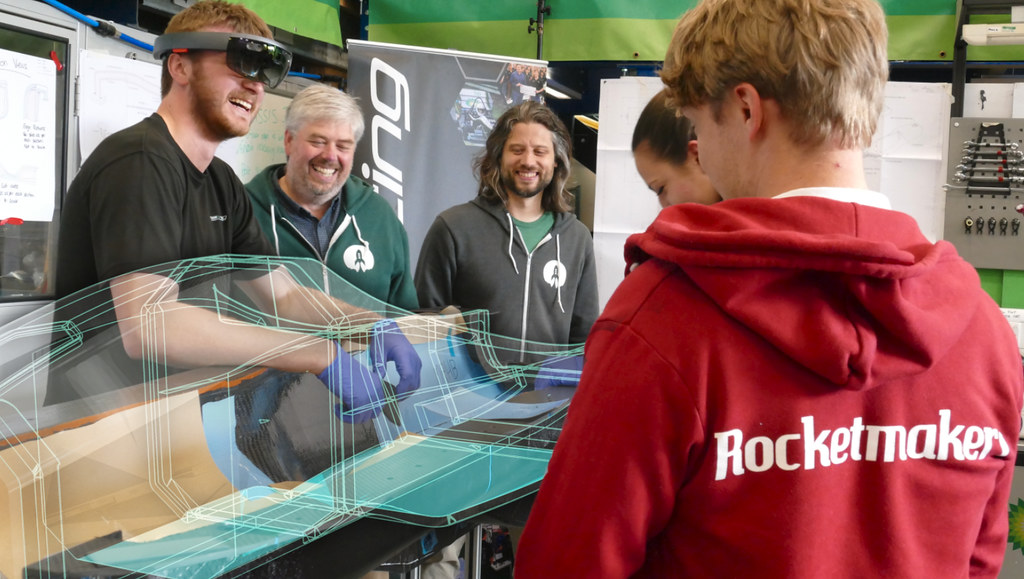
\includegraphics[width=0.6\linewidth]{carAR}
    \caption{Construcción de un automóvil de carreras gracias a la RA.}
    \label{fig:xyz}
\end{figure}    
 

\subsubsection{AR Sandbox} 
AR Sandbox \cite{URL::sandbox} es el resultado de un proyecto desarrollado por W.M. El Centro Keck para la Visualización Activa en las Ciencias de la Tierra (KeckCAVES), junto con el Centro de Investigación Ambiental UC Davis Tahoe, Lawrence Hall of Science y ECHO Lake Aquarium and Science Center.

El proyecto combina aplicaciones de visualización 3D con una exhibición de AR Sandbox para enseñar conceptos de ciencias de la tierra. La caja de arena de realidad aumentada  permite a los usuarios crear modelos de topografía al dar forma a la arena real, que luego se aumenta en tiempo real mediante un mapa de color de elevación, líneas de contorno topográficas y agua simulada. El sistema enseña conceptos geográficos, geológicos e hidrológicos, como la forma de leer un mapa topográfico, el significado de las curvas de nivel, las cuencas hidrográficas, los diques, etc.

\begin{figure}[h]
    \centering
    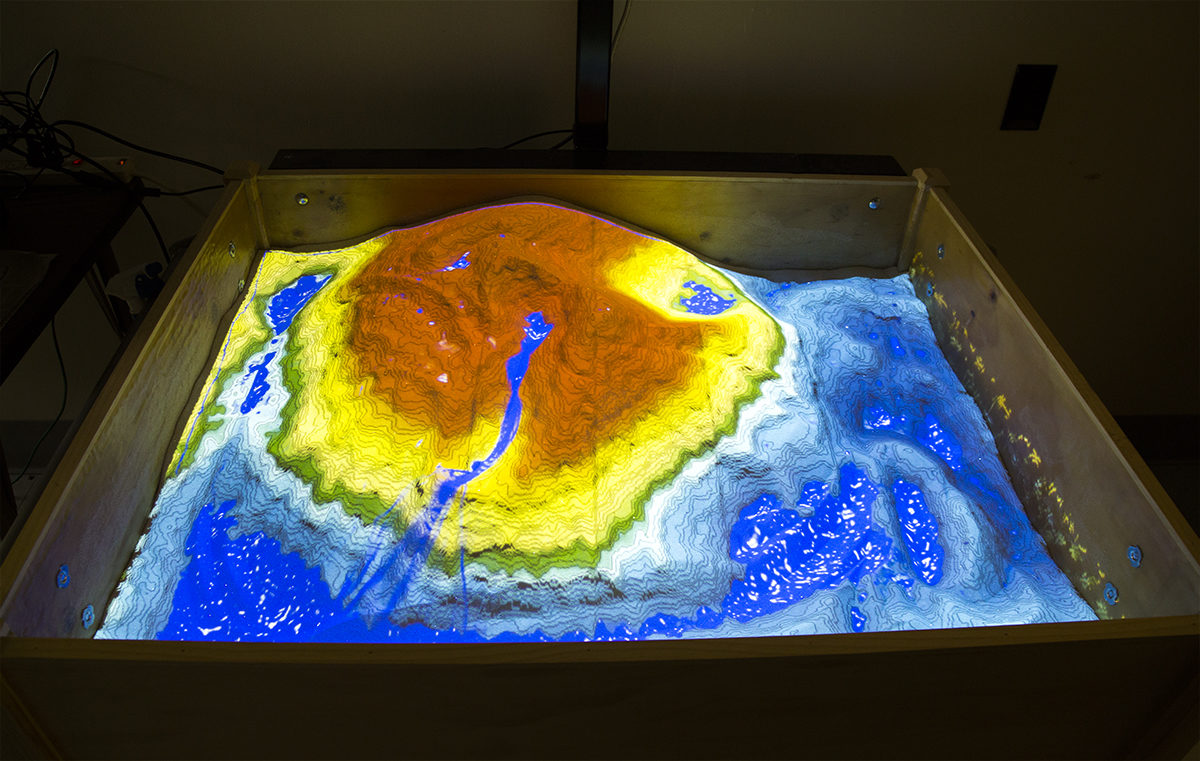
\includegraphics[width=0.8\linewidth]{sandAR}
    \caption{Funcionamiento de AR Sandbox.}
    \label{fig:xyz}
\end{figure}    


% Varios científicos de la Universidad Carlos III de Madrid han diseñado unas gafas inteligentes que permiten conectar a profesores y alumnos en tiempo real en el aula. Telmo Zarraonandia, Ignacio Aedo, Paloma Díaz y Álvaro Montero a través del artículo, An augmented lecture feedback system to support learner and teacher communication explican su funcionamiento. Con tan solo ponerse las gafas en cuestión, el docente obtendrá información del alumno al mirar tras ellas. Notas y comentarios que lanzarán los alumnos al docente los podrá recibir con tan solo observar a su grupo de clase.

% El feedback estará asegurado en estas aulas, de nuevo utilizando como recurso tecnológico la realidad aumentada.

% % https://e-archivo.uc3m.es/bitstream/handle/10016/17136/augmented_british_2013_pp.pdf?sequence=1&isAllowed=y

% https://www.itv.com/news/2019-05-09/students-use-augmented-reality-tool-to-help-manufacture-race-car/

% Collaborative work of students within the
% Augmented Reality application Construct3D

% Libros de texto aumentados 


% Modelos 3D utilizados en arquitectura para la visualización de dispositivos







% ---------------------------------------------------
%
% Trabajo de Fin de Grado. 
% Author: Alejandro Hernández Padrón. 
% Capítulo: La aplicación ULL-AR. 
% Fichero: Cap4_TheApplication.tex
%
% ----------------------------------------------------
%


\lstset{stringstyle=\color{purple}}
\chapter{La aplicación ULL-AR} \label{chap:LaAplicacion} 

En este capítulo explicaremos la aplicación ULL-AR utilizando la especificación de requisitos de esta y explicando su funcionamiento.

\section{Requisitos y ventanas de la aplicación} % (fold)


Se trata de una aplicación para móviles, más concretamente, a aquellos dispositivos que utilizan Android como sistema operativo. Es una aplicación diseñada para la comunidad de la Universidad de La Laguna, la cual les permita ubicarse, detectar y reconocer las instalaciones y edificios pertenecientes a la universidad, mediante técnicas de realidad aumentada basadas en la geolocalización.

Los requisitos principales de ULL-AR son:
\begin{itemize}
    \item La aplicación se desarrollará para dispositivos con Android. Se utilizará Android Studio como IDE para su desarrollo.
    \item Se implementarán técnicas de realidad aumentada basadas en la geolocalización para mostrar al usuario la instalación de la ULL a la cual apunte con la cámara.
    \item Las instalaciones, junto a su información correspondiente, estarán ubicadas en un base datos en la nube. El servidor que se conecte con esta base de datos también deberá estar en la nube.
\end{itemize}

\subsection{Especificación detallada de los requisitos} 

La aplicación se iniciará una Splash Screen \cite{URL::SplashScreen} o pantalla de inicio con el logo de la Universidad de La Laguna. Esta pantalla dará paso a una ventana de \textit{Inicio de sesión}.

Para poder utilizar ULL-AR, el usuario ha de tener una cuenta de correo institucional de la ULL. Este correo ha de tener el siguiente formato: ``\textit{aluxxxxxxxxxx@ull.edu.es}''. Sin ella no se podrá acceder a la aplicación. Además, se podrá cerrar la sesión de esta cuenta.

Una vez autentificado con éxito, se accederá a una ventana de \textit{Inicio} en la que aparecerá un acceso directo a las ventanas de \textit{Mapa ULL} y \textit{Navegación en modo RA} que explicaremos más adelante. A su vez, dispondrá de los accesos directos a enlaces de interés de Universidad de La Laguna que se abrirán en un navegador externo. 

ULL-AR cuenta con un menú para moverse por las diferentes ventanas. Se implementará un menú deslizante lateral o \textit{Navigation Drawer} \cite{URL::NavigationDraw} ubicado en la parte superior izquierda de la aplicación. Este menú deberá ser simple e intuitivo.

Como accesos en este menú se dispone de las siguientes ventanas:

\begin{itemize}
    \item Inicio: Ventana principal de la aplicación.
    \item Mapa ULL: Esta ventana contendrá un mapa de la universidad con todas las instalaciones en la base de datos. 
    \item Navegación en modo RA: En esta ventana, mediante el uso de la cámara, se identificarán las instalaciones universitarias a los que el usuario apunte y permitirá mostrar una pestaña con información detallada de las mismas.
    \item Todas las instalaciones ULL: Contiene todas la ubicaciones e instalaciones de la Universidad de La Laguna y permitirá la búsqueda de estas. 
    \item Configuración: Permitirá acceder a los ajustes de la aplicación.
    \item Cerrar cesión: Cerrará la sesión actual y devolverá al usuario a la ventana de \textit{Inicio de sesión}.
    \item Info: Información de la aplicación y de su autor.
\end{itemize}

Una instalación de la ULL corresponde a un centro, edificio, facultad, instituto, polideportivo, etc. Cada instalación de la universidad tendrá una ficha de información que será accesible desde una ventana de la aplicación con la siguiente información:

\begin{itemize}
    \item \textbf{Id}: Campo para identificar la instalación.
    \item \textbf{Nombre}: Nombre oficial de la instalación.
    \item \textbf{Ubicación}: La ubicación exacta en la que se encuentra la instalación. 
    \item \textbf{Descripción}: Descripción de la instalación con el objetivo y actividades que se desarrollan en él.
    \item \textbf{Imagen}: Imagen de la instalación.
    \item \textbf{Lista de enlaces de interés}: Una lista con los enlaces a las instituciones, servicios, departamentos y grados que se imparten en esta instalación.
\end{itemize}

Esta información estará guardada en una base de datos en la nube. Para acceder a esta, se dispondrá de un servidor en la nube que conecte con la base de datos y envié la información a la aplicación.

\subsection{Ventanas de la aplicación}

 

% \begin{figure}[h]
% \hspace*{\fill}%
% \begin{subfigure}[h]{0.32\linewidth}
% 
\includegraphics[width=\linewidth]{splashApp}
% \caption{Splash-Screen.}
% \label{fig:splashApp}
% \end{subfigure}
% \hfill%
% \begin{subfigure}[h]{0.32\linewidth}
% 
\includegraphics[width=\linewidth]{loginApp}
% \caption{Login.}
% \label{fig:loginApp} 
% \end{subfigure}%
% \caption{Ventanas de iniciales de \textit{ULL-AR}.}
% \hspace*{\fill}%
% \end{figure}
  
% La primera ventana (véase Figura \ref{fig:splashApp}) es la pantalla de inicio o Splash Screen que aparece cuando ejecutamos la aplicación. Tras unos segundos, se carga la ventana de \textit{Login} (véase Figura \ref{fig:loginApp}). Para poder loguearnos deberemos tener una cuenta de Google de la ULL. Una vez que presionamos en el botón del medio, se nos abrirá una ventana de diálogo para que pongamos nuestra cuenta.

Al iniciar la aplicación ULL-AR, la primera ventana que aparece es la pantalla de inicio o Splash Screen. Tras unos segundos, se carga la ventana de \textit{Inicio de sesión}. Para poder auntificarse el usuario debe poseer una cuenta de correo institucional de la ULL.
Se dispondrá de un botón en el centro de la pantalla, que abrirá un cuadro de diálogo en el que poder introducir el correo y contraseña de esta cuenta.
  
\begin{figure}[h]
    \hspace*{\fill}%
    \begin{subfigure}[h]{0.35\linewidth}
    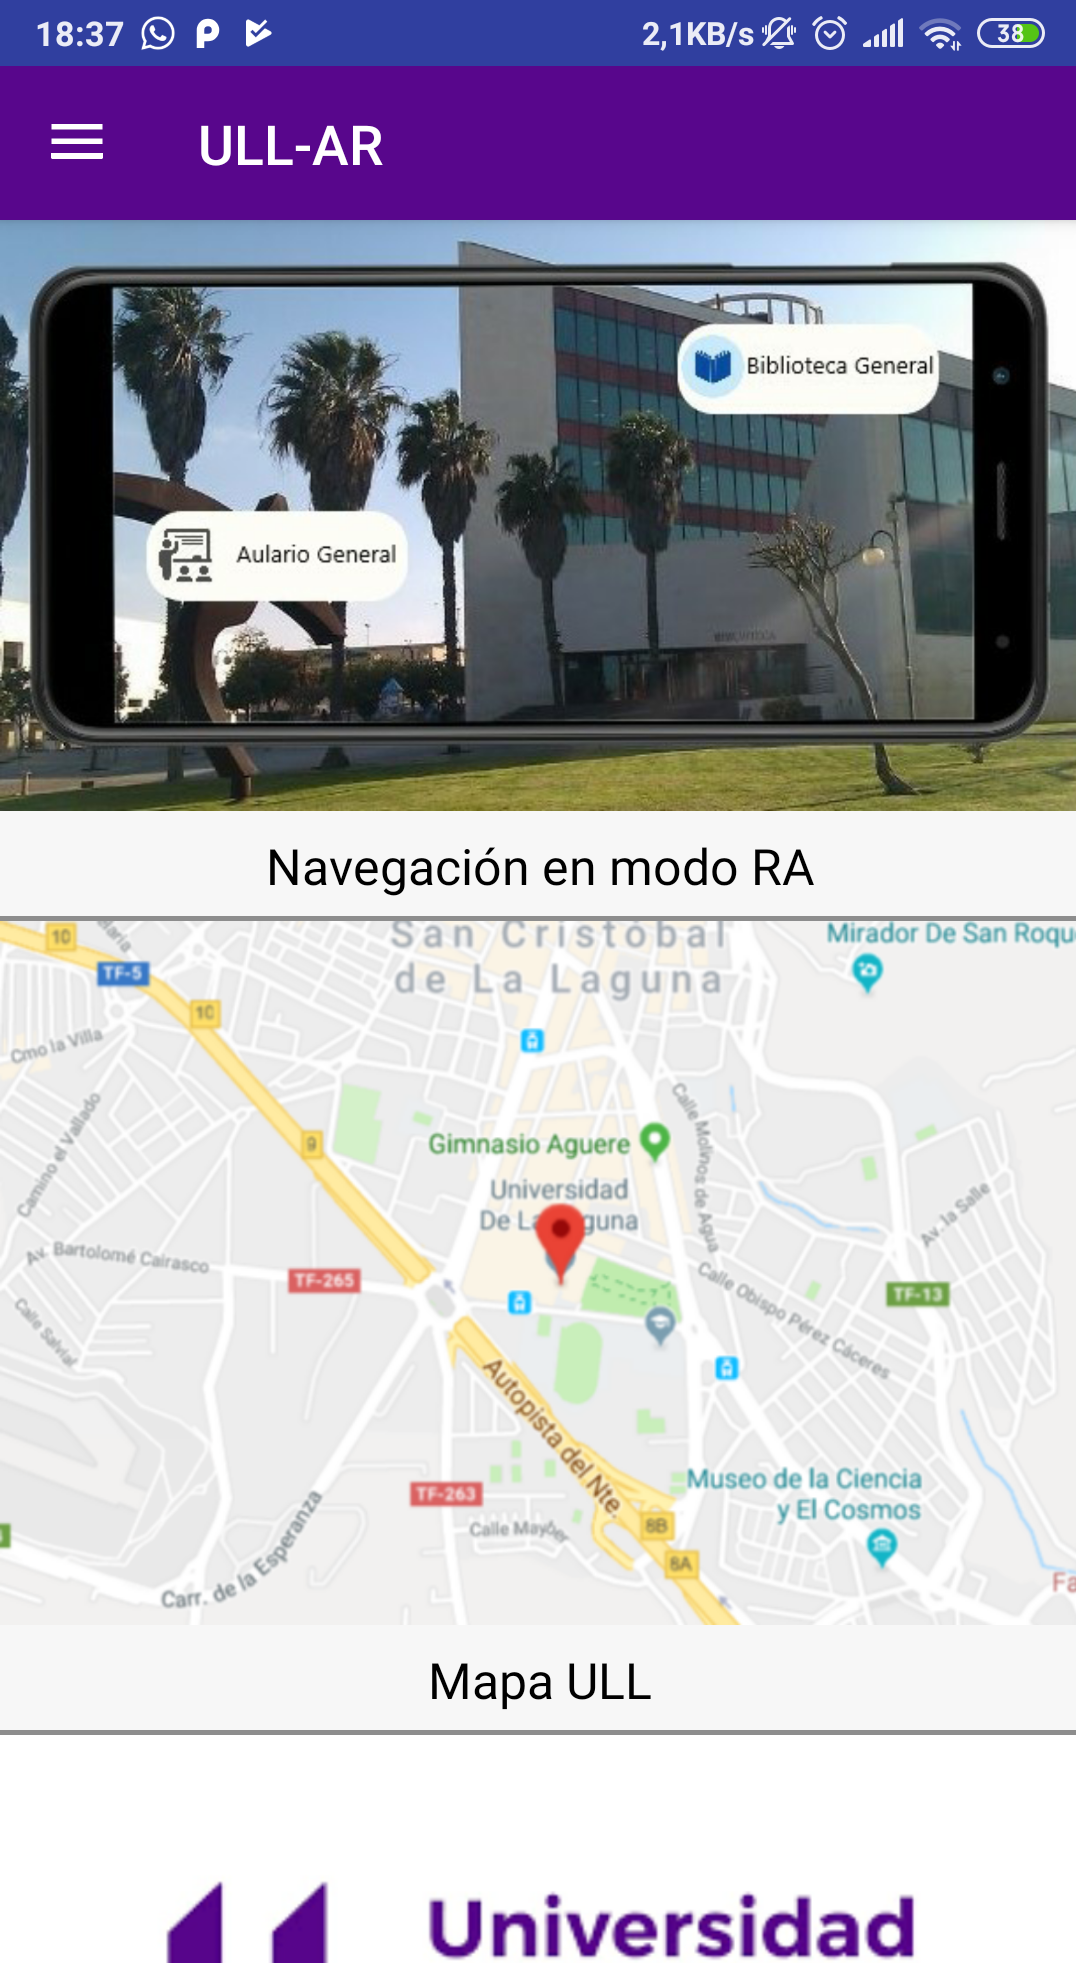
\includegraphics[width=\linewidth]{homeApp}
    \caption{Inicio.}
    \label{fig:homeApp}
    \end{subfigure} 
    \hfill%
    \begin{subfigure}[h]{0.35\linewidth}
    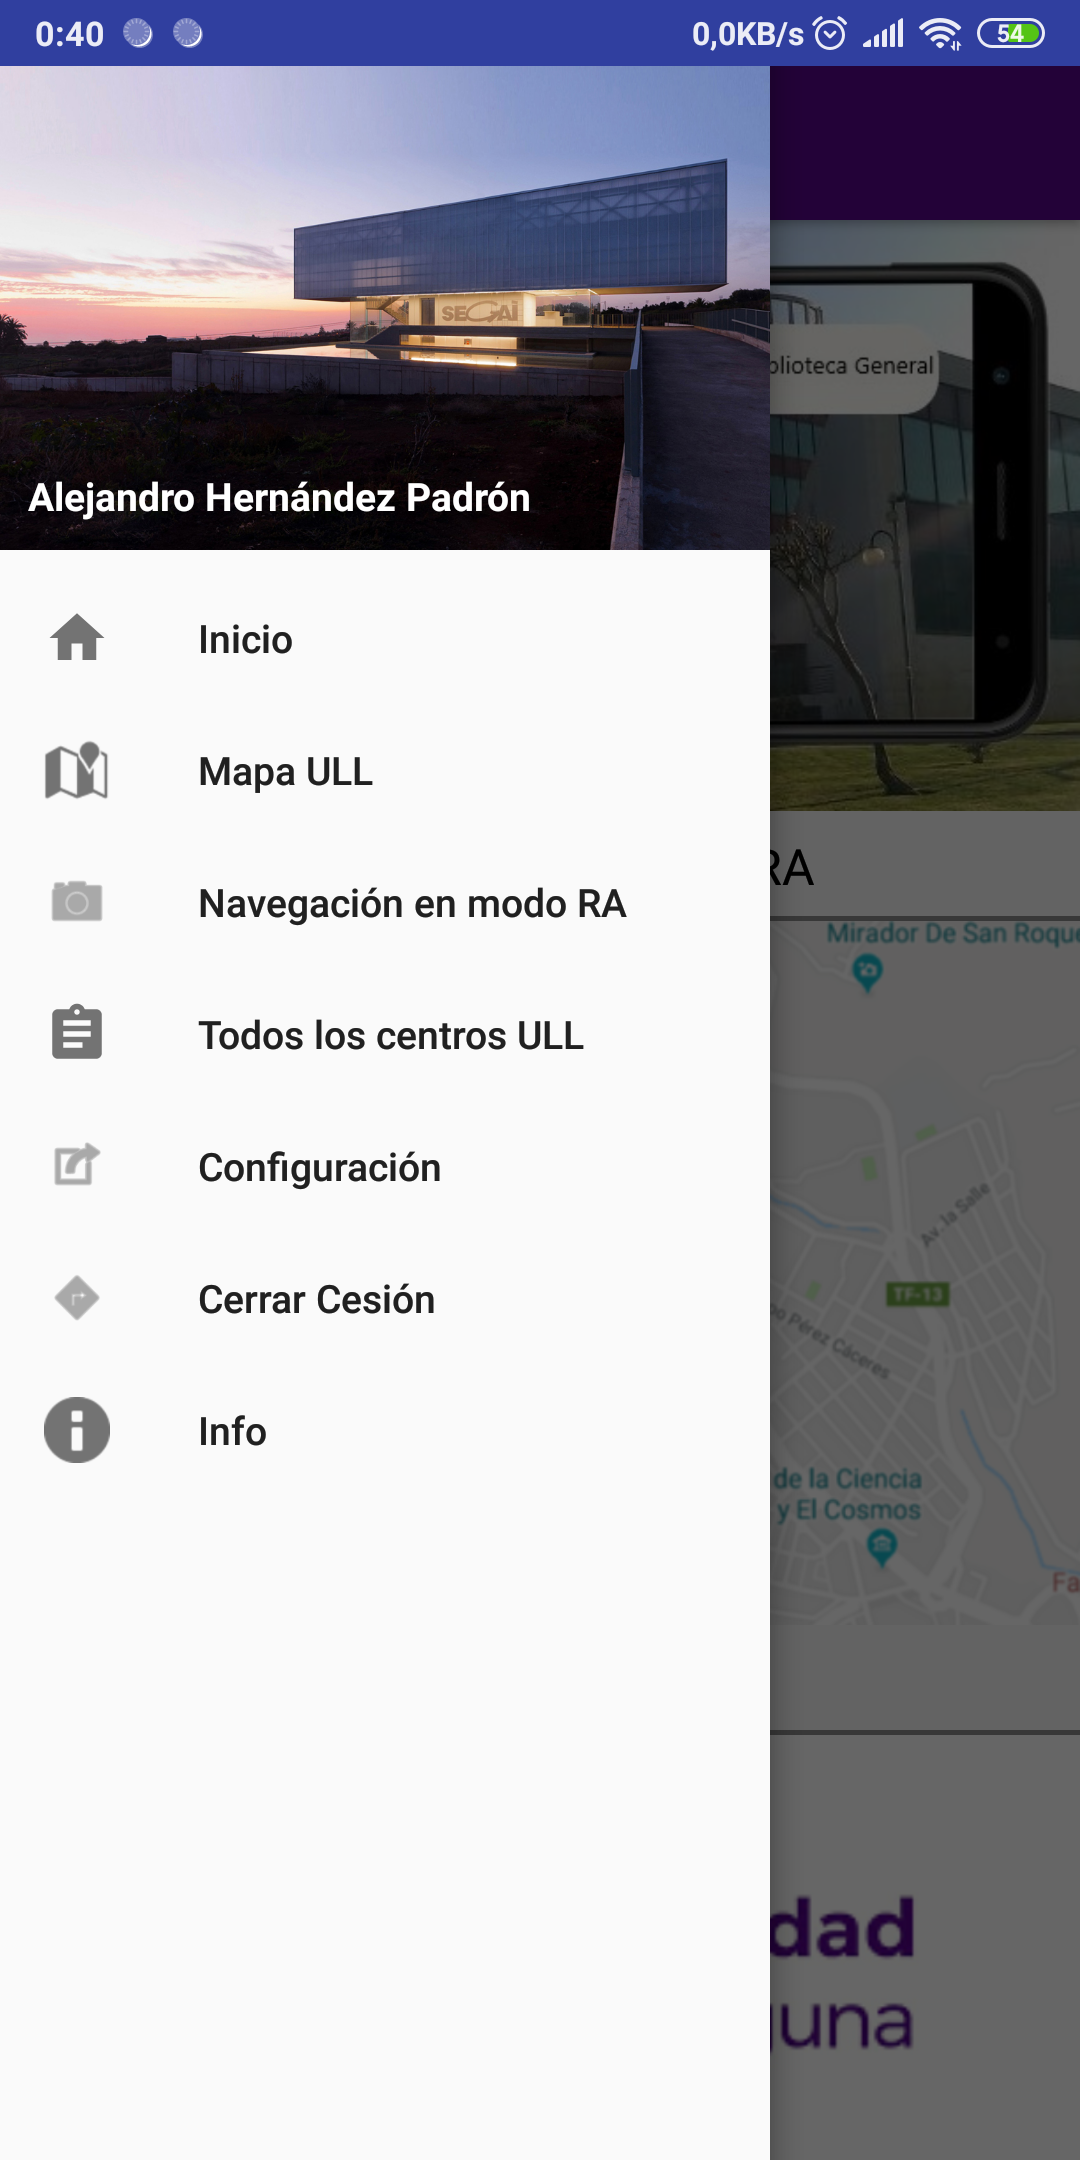
\includegraphics[width=\linewidth]{menuApp}
    \caption{Menu. Navigation Drawer.}
    \label{fig:menuApp}
    \end{subfigure}%
    \caption{Ventana \textit{Inicio} y el \textit{Menú} de \textit{ULL-AR}.}
    \hspace*{\fill}%
\end{figure}

Cuando el usuario consiga autentificarse con éxito, se abrirá la ventana de \textit{Inicio} (véase Figura \ref{fig:homeApp}). En ésta aparecerá una lista de accesos directos a las funcionalidades principales de ULL-AR, como son \textit{Navegación en modo RA} y \textit{Mapa ULL}, y una serie de enlaces a sitios web relacionados con la ULL.

En la esquina superior izquierda de ULL-AR se encuentra situado el botón de acceso al menú \textit{Navigation Drawer}. Si se presiona se desplegará el menú que permite al usuario moverse por las distintas ventanas de la aplicación (véase Figura \ref{fig:menuApp}).

Si el usuario se desplaza a la ventana de \textit{Mapa ULL} (véase Figura \ref{fig:mapsApp}) encontrará el mapa generado por la API de Google Maps. En este mapa aparecerá en pines azules las instalaciones de la ULL que están guardadas en la base de datos. Cuando el GPS del dispositivo encuentre la ubicación actual, aparecerá un pin rojo que indicará su posición en el mapa. En la parte inferior y en el centro de la ventana, se dispone de un botón llamado ``AR Mode'' que permite acceder a la ventana de \textit{Navegación en modo RA}.
  
\begin{figure}[h]
    \hspace*{\fill}%
    \begin{subfigure}[h]{0.37\linewidth}
        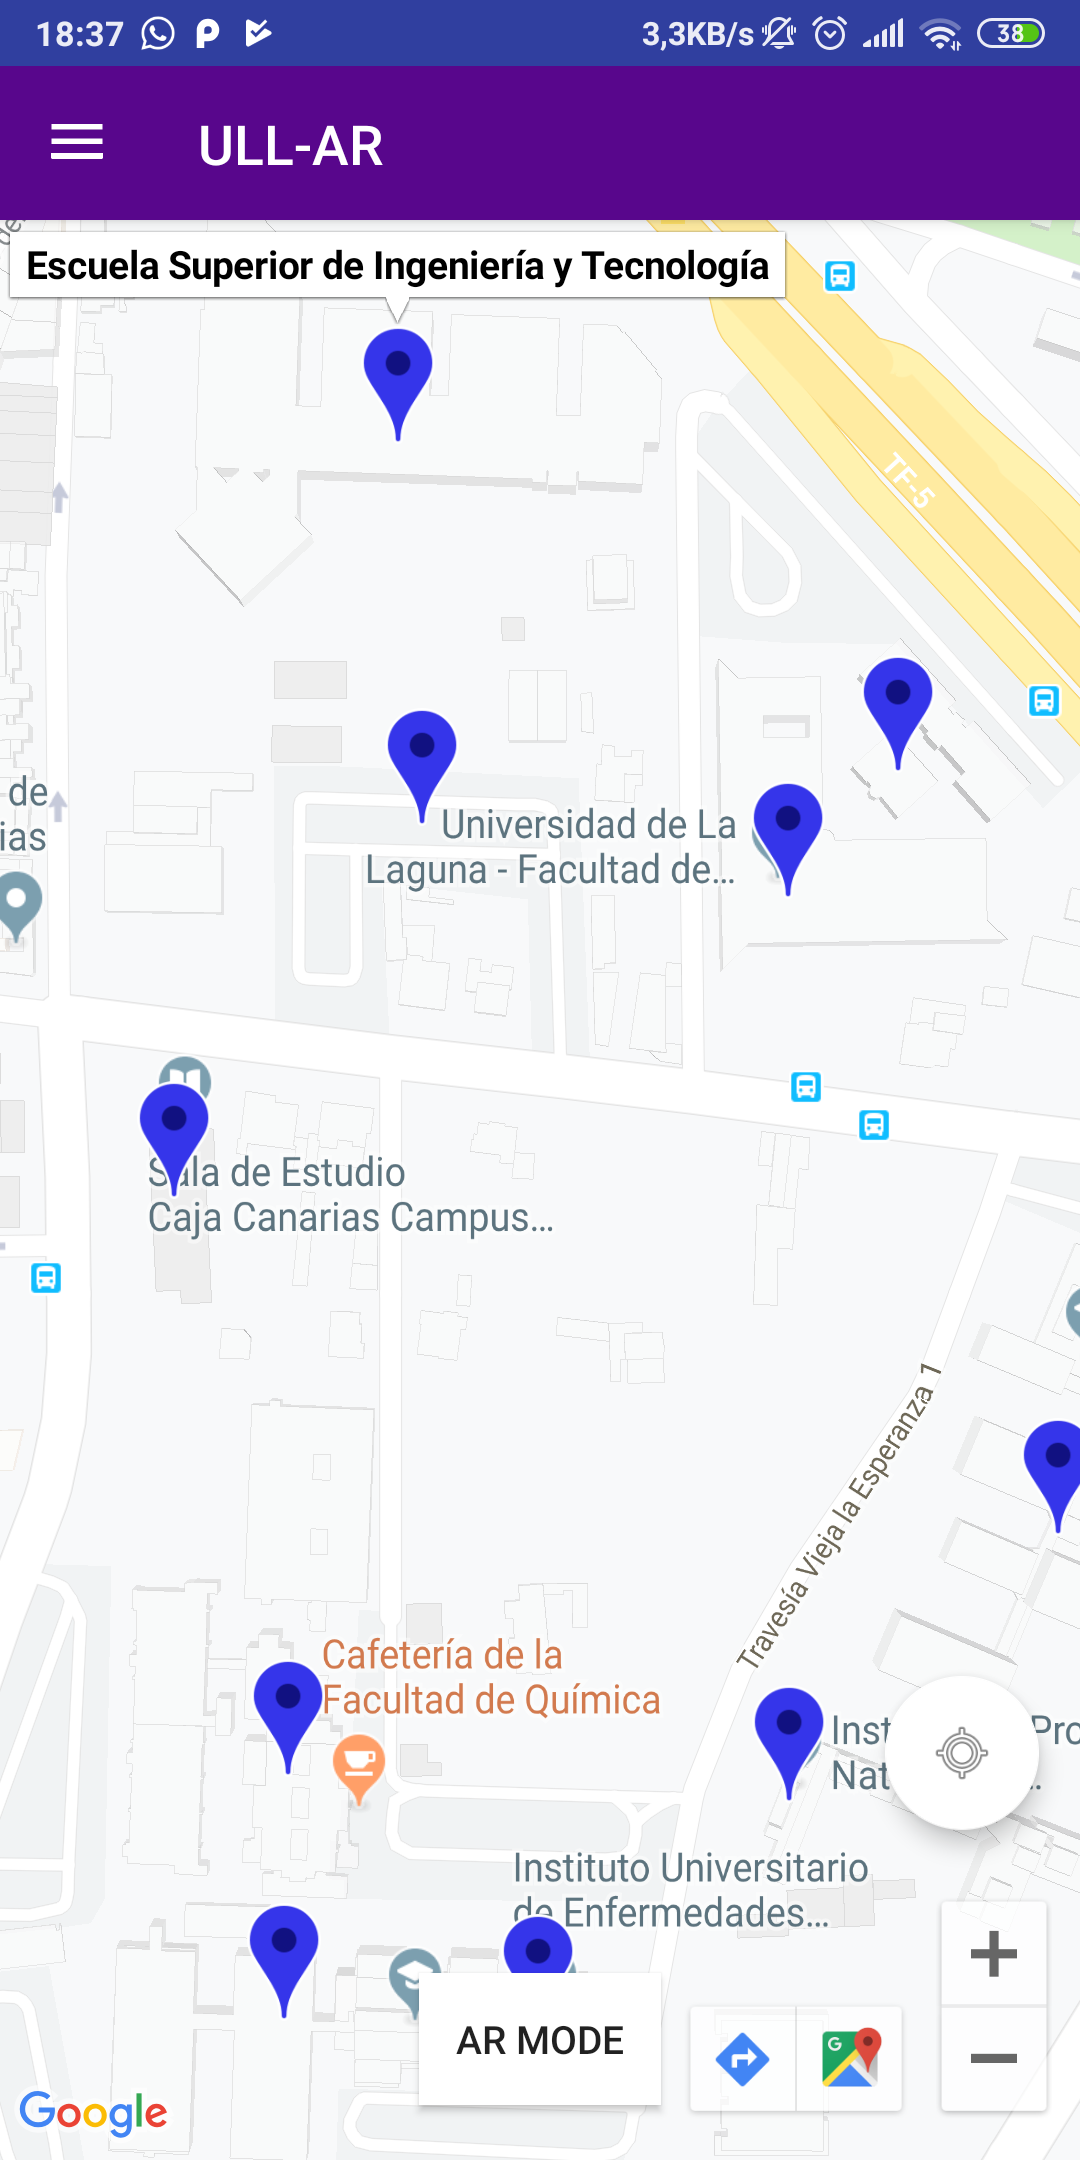
\includegraphics[width=\linewidth]{mapsApp}
        \caption{Mapa ULL.}
        \label{fig:mapsApp}
    \end{subfigure}
    \hfill%
    \begin{subfigure}[h]{0.37\linewidth}
        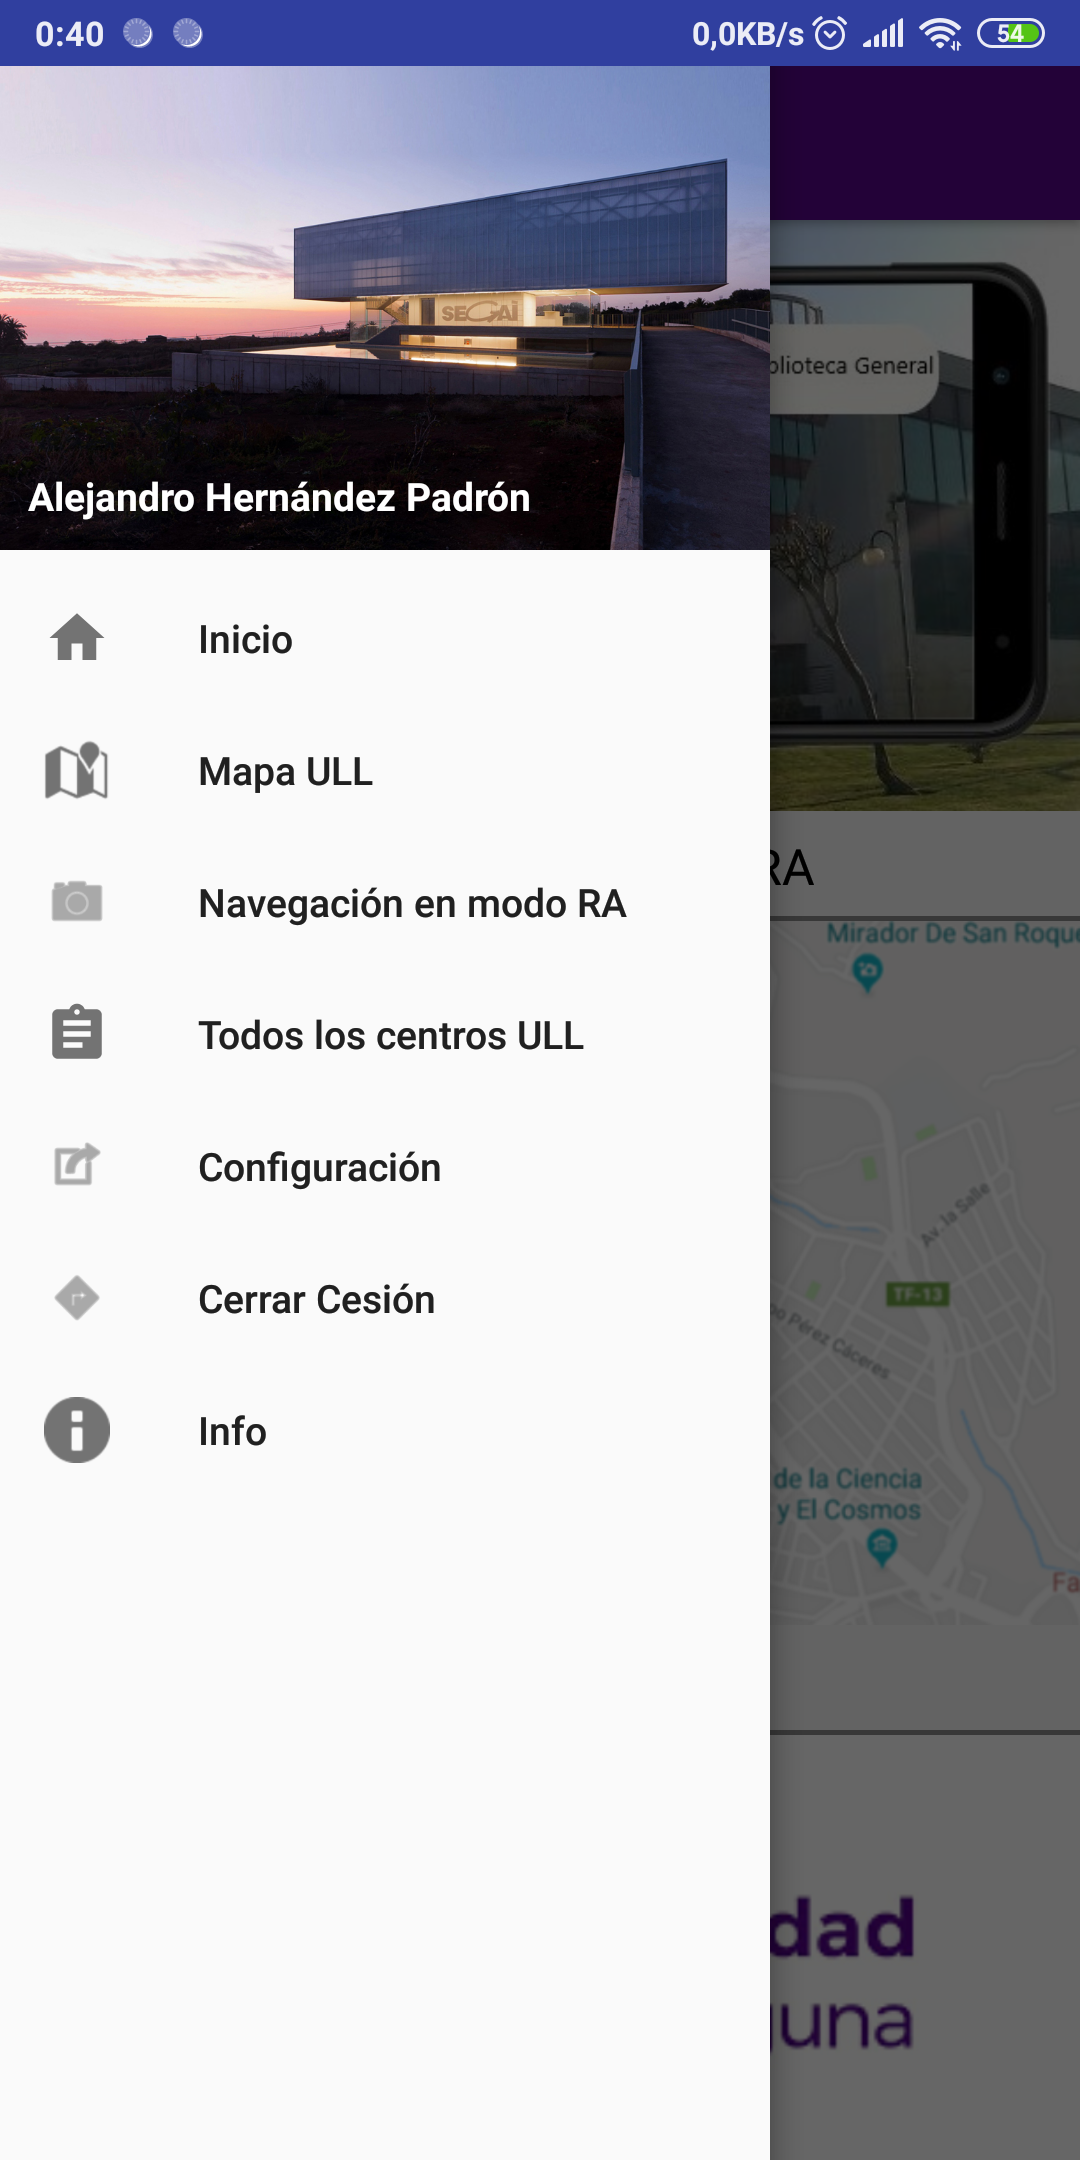
\includegraphics[width=\linewidth]{menuApp}
        \caption{Ventana de \textit{Inicio}}
        \label{fig:menussApp}
    \end{subfigure}%
    \caption{Ventana Inicio y menú de \textit{ULL-AR}}
    \hspace*{\fill}%
\end{figure}

% \begin{figure}[h]
%     \centering
%     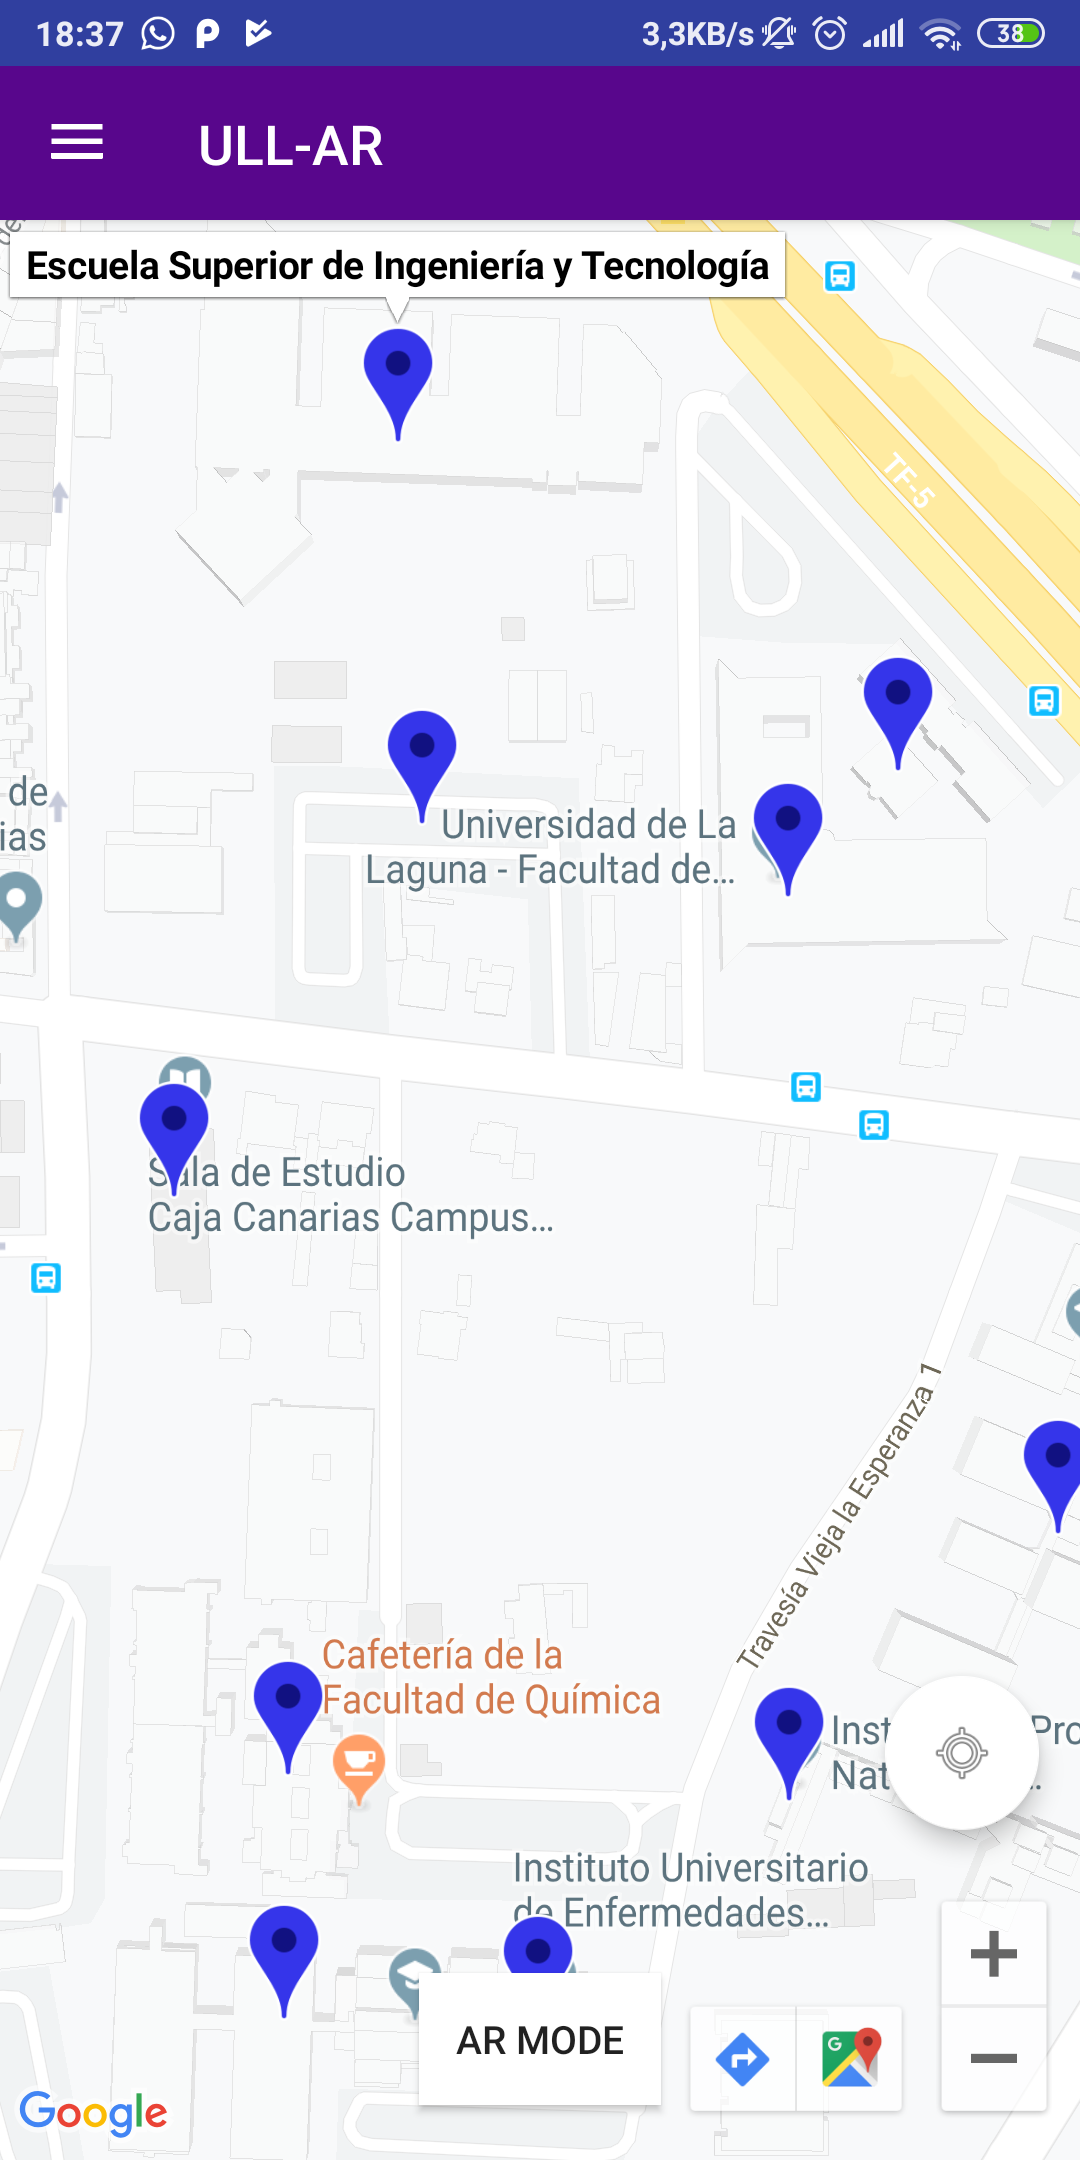
\includegraphics[width=0.38\linewidth]{mapsApp}
%     \caption{Mapa ULL.}
%     \label{fig:mapsApp}
% \end{figure}

En la ventana de \textit{Navegación en modo RA} se mostrará la imagen obtenidad de la cámara del dispositivo, con ella el usuario podrá ver en la pantalla la instalación a la que se apunte. Encima de esta imagen se mostrará un texto en el que aparecerán dos mensajes: uno informativo para indicar a usuario que apunte a alguna instalación de la ULL y una vez que se el usuario se encuentre apuntando a una instalación, el mensaje anterior se cambiará por el nombre de la instalación y, al mismo tiempo, aparecerá un pequeño boton debajo del texto que llevará al usuario a la ventana de \textit{Información de la instalación} (véase Figura \ref{fig:siteInfoApp}), con la información de dicha instalación. Por último, en la parte inferior se mostrará un botón que indicará si se han encontrado más instalaciones a parte de la que se muestra en la parte superior. Esté botón ejecutará una ventana con una lista de estas instalaciones.

 
\begin{figure}[h]
    \hspace*{\fill}%
    \begin{subfigure}[h]{0.37\linewidth}
    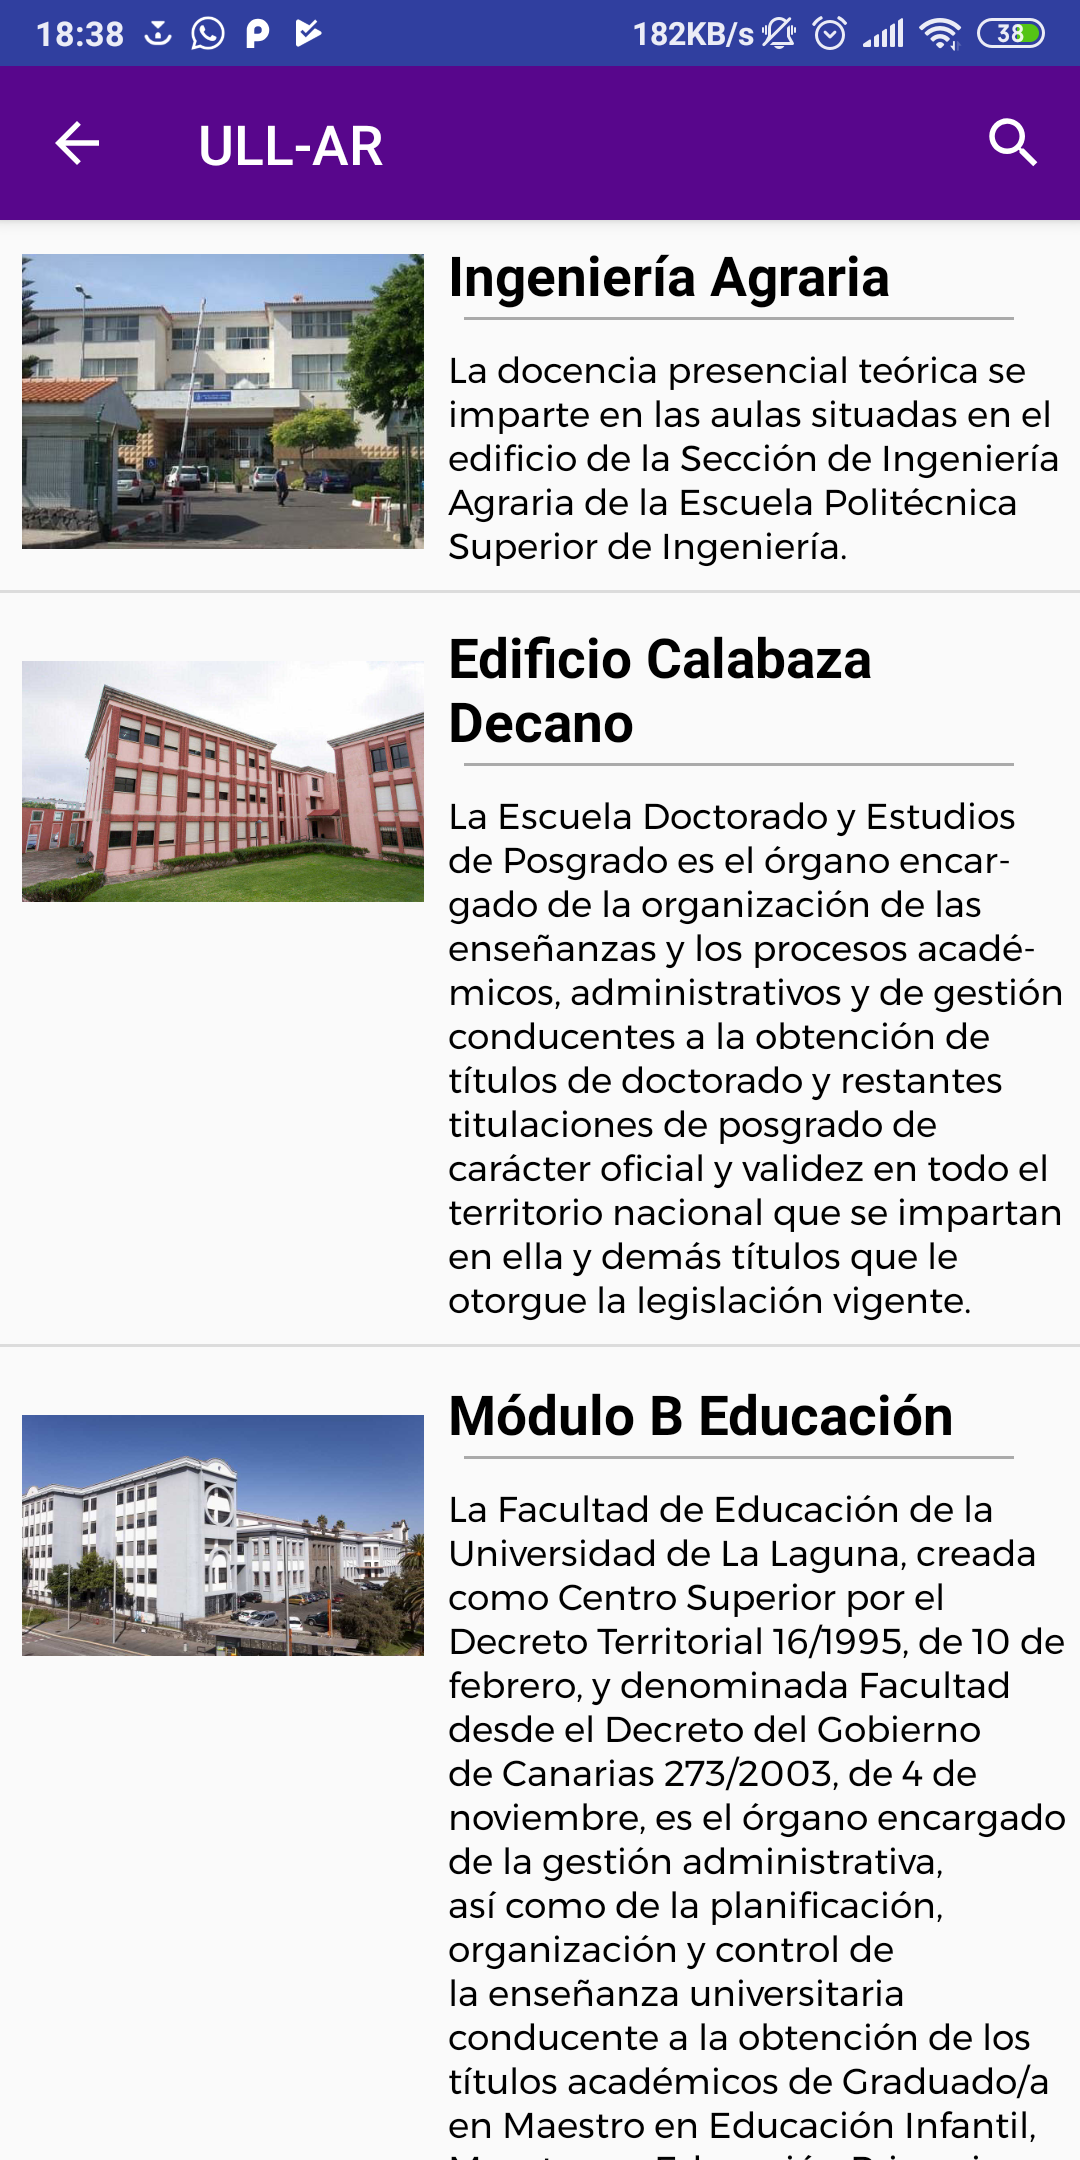
\includegraphics[width=\linewidth]{allSitesApp}
    \caption{Todas las instalaciones ULL.}
    \label{fig:allSitesApp}
    \end{subfigure}
    \hfill%
    \begin{subfigure}[h]{0.37\linewidth}
    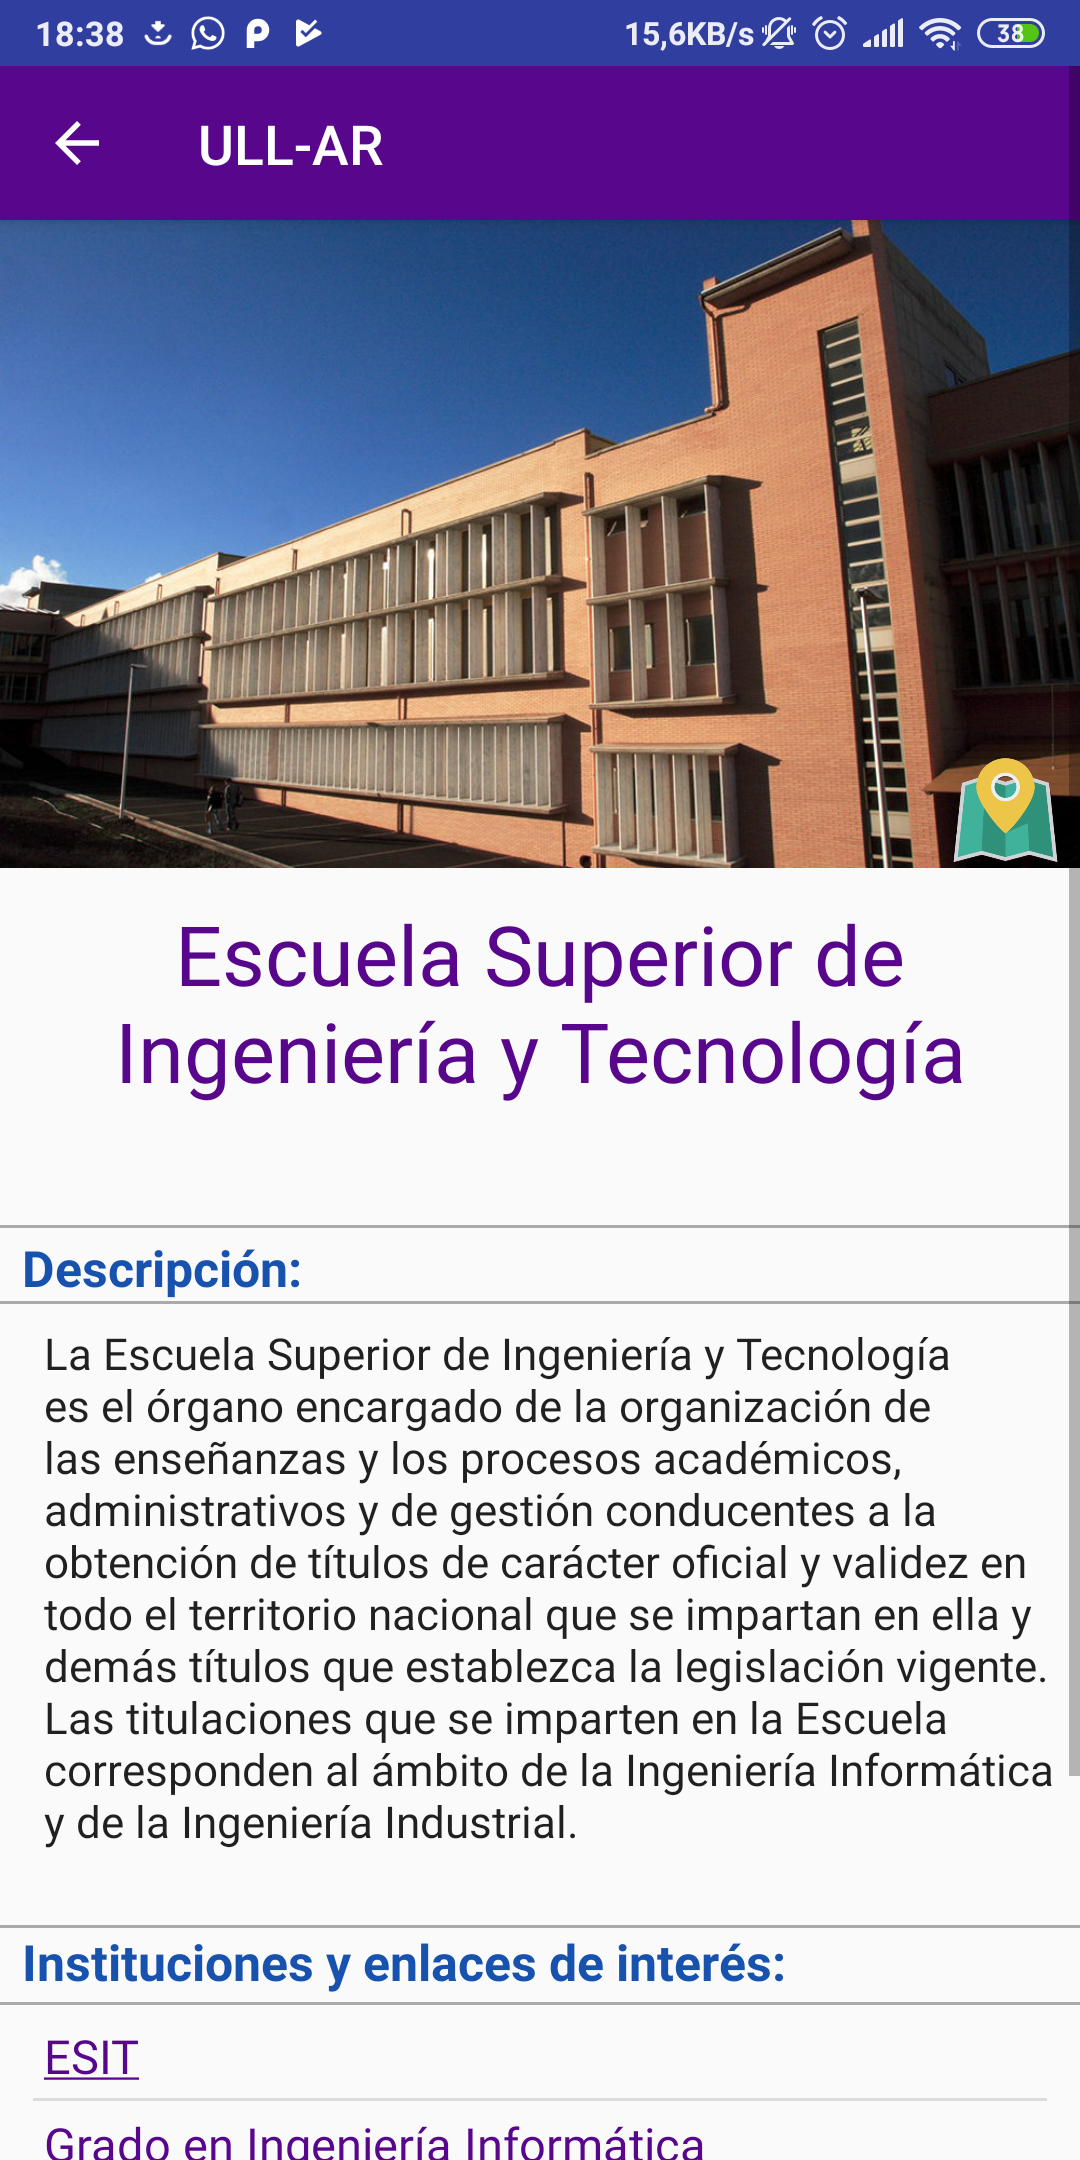
\includegraphics[width=\linewidth]{siteInfoApp}
    \caption{Información de la instalación.}
    \label{fig:siteInfoApp}
    \end{subfigure}%
    \caption{Ventanas de \textit{Todas las instalaciones ULL} e \textit{Información de la instalación} de \textit{ULL-AR}.}
    \hspace*{\fill}%
\end{figure}

\vskip 0.9in

A través del menú de la aplicación se puede acceder a la ventana de \textit{Todas las instalaciones ULL} (véase Figura \ref{fig:allSitesApp}). Aquí se mostrarán todas las instalaciones de la ULL que se encuentran en la base de datos. Además, se podrá hacer una búsqueda de cualquier instalación en la barra superior de la aplicación. Si se presiona cualquiera de estas instalaciones se  desplegará una ventana con la información detallada de la instalación.



La ventana \textit{Información de la instalación} (véase Figura \ref{fig:siteInfoApp}) se dispondrá la información perteneciente a cada instalación. Aquí se  mostrará una imagen de ésta, nombre y descripción de la instalación y una lista de enlaces con los servicios, secretarias, grados y departamentos que podemos encontrar. Disponemos de un botón en la parte inferior de la imagen de la instalación, que  abrirá la ruta a su ubicación en la aplicación de Google Maps para poder llegar a ella.  



Por último, desde el menú se puede acceder a las ventanas de \textit{Configuración} e \textit{Información}.

En la ventana de \textit{Configuración} (véase Figura \ref{fig:settingsApp}) se encuentran los ajustes de la aplicación. En ella tenemos la opción para poder configurar si queremos encontrar las instalaciones que se encuentran en el área entre dos circunferencias.

La ventana \textit{Info} (véase Figura \ref{fig:infoApp})  muestra información básica de la aplicación como el nombre, versión, correo de contacto, autor y objetivo e información del desarrollo de la aplicación \textit{ULL-AR}.  

\begin{figure}[h]
    \hspace*{\fill}%
    \begin{subfigure}[h]{0.35\linewidth}
    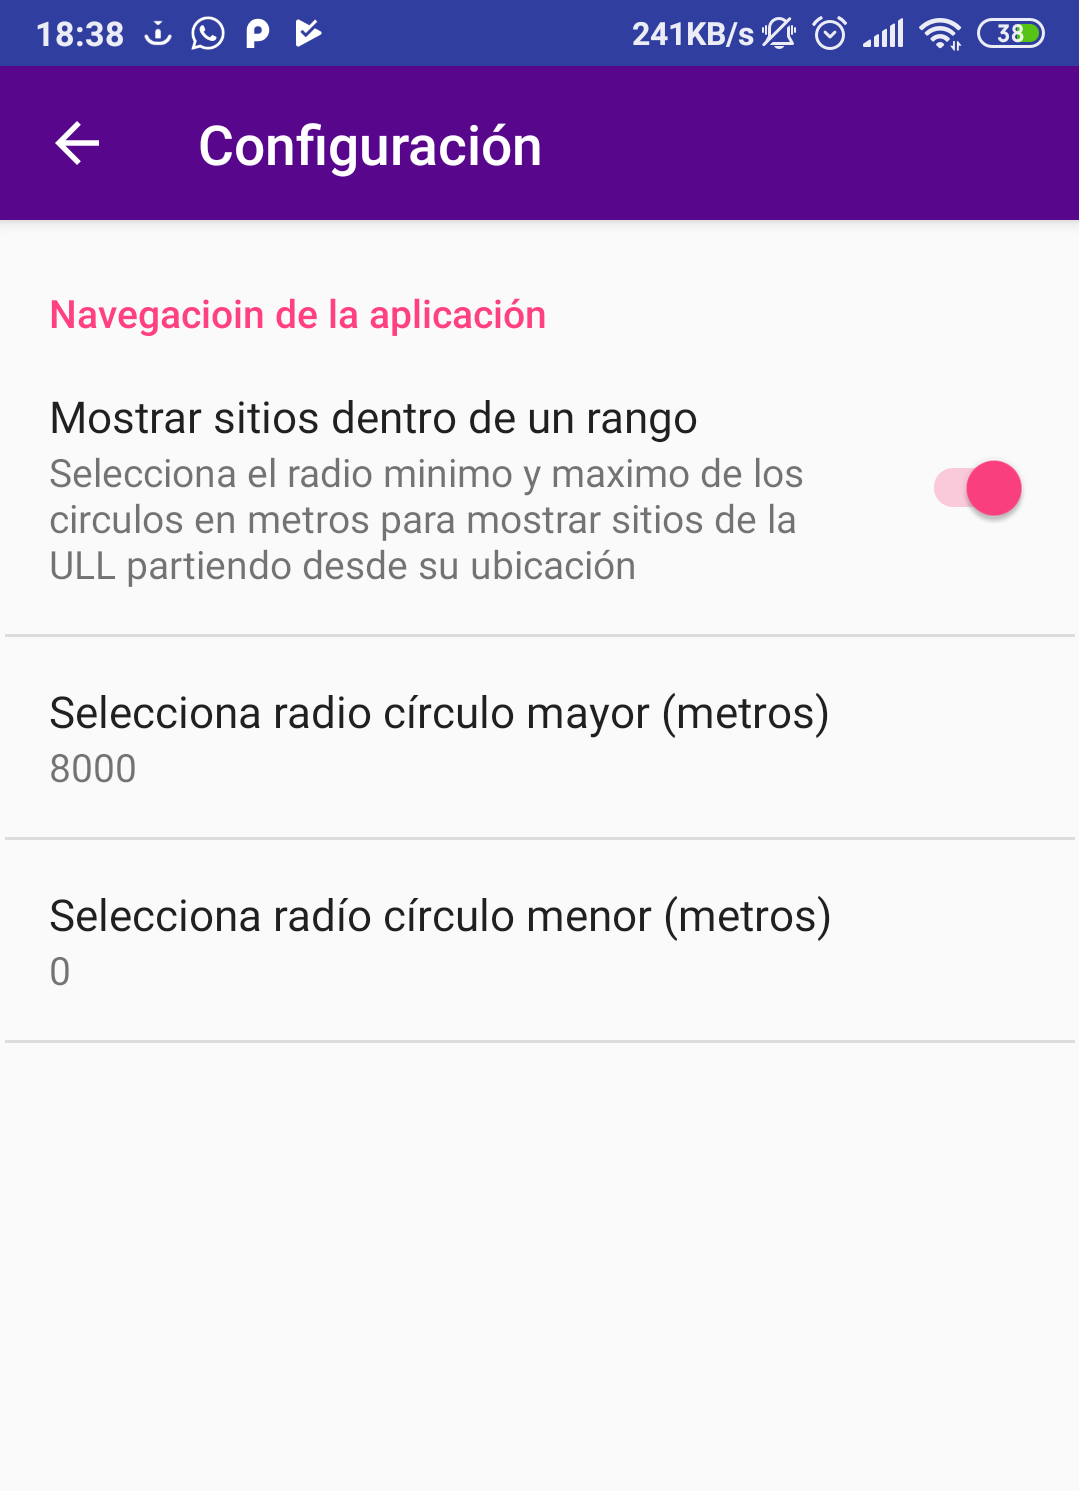
\includegraphics[width=\linewidth]{settingsApp}
    \caption{Configuración.}
    \label{fig:settingsApp}
    \end{subfigure}
    \hfill%
    \begin{subfigure}[h]{0.35\linewidth}
    
\includegraphics[width=\linewidth]{infoApp}
    \caption{Información.}
    \label{fig:infoApp}
    \end{subfigure}%
    \caption{Ventanas de \textit{Configuración} e \textit{Info} de \textit{ULL-AR}.}
    \hspace*{\fill}%
\end{figure}


\vskip 1.9in

\section{Inicio de ULL-AR} \label{chap:StartApplication} 

Para comenzar a desarrollar aplicación, primero, necesitamos crear un proyecto nuevo en Android Studio. Este proyecto lo nombramos con el nombre de nuestra aplicación ``ULL-AR'' y seguiremos los pasos del IDE para acabar de crear nuestro proyecto. 

A continuación, explicaremos en detalle el funcionamiento e implementación de las primeras ventanas que aparecen cuando se inicia la aplicación. 

\subsection{Ventana inicial}

La primera ventana que aparece en la aplicación es la \textit{Splash Screen}. El objetivo de esta ventana es dar una mejor apariencia a la aplicación e informar al usuario que la aplicación se esta inciando y cargando. 

En esta ventana encontraremos el logotipo de ULL-AR (véase Figura \ref{fig:logoApp}) en el centro de la pantalla. Este logo se ha diseñado por medio del editor de imagenes online Pixlr \cite{URL::pixlr}. Gracias a este programa hemos podido crear un logotipo simple combinando el icono de la marca de la ULL y el nombre de la aplicación.
 
\begin{figure}[h]
    \centering
    
\includegraphics[width=0.3\linewidth]{logoApp}
    \caption{Logo de ULL-AR.}
    \label{fig:logoApp}
\end{figure}    
 

En un principio la velocidad de carga y transición a la siguiente ventana de la aplicación se hacía de forma inmediata. Esto se produce por que los recursos necesarios para el inicio de la aplicación son escasos y no tardan en cargarse. Por lo tanto, para poder visualizarla correctamente se utilizó un temporizador de tres segundos, para que posteriormente, se lance la siguiente ventana, que corresponde a la ventana de \textit{Inicio de sesión}.

Para la implementación de esta ventana se ha de configurar primero el archivo \texttt{AndroidManifest.xml}, este fichero proporciona información esencial sobre tu aplicación al sistema Android, información que el sistema debe tener para poder ejecutar el código de la aplicación. Aquí le indicamos al sistema Android la ventana o ``activity'' \cite{URL::activity} que se inicia la aplicación (véase Listado \ref{lst:manifestInicio}). Además, a esta ventana se le indica el tema del activity que contendrá el logotipo de ULL-AR en el centro de la pantalla.

\begin{lstlisting}[language=XML,caption={Fichero \texttt{AndroidManifest.xml}, activity que inicia la aplicación.}, label={lst:manifestInicio}]
    ...
    <activity
        android:name=".Activities.SplashActivity"
        android:theme="@style/SplashScreen">
        <intent-filter> 
            <action android:name="android.intent.action.MAIN" />
            <category android:name="android.intent.category.LAUNCHER" />
        </intent-filter>
    </activity>
    ...
\end{lstlisting}

Al mismo tiempo en el archivo \texttt{styles.xml} (véase Listado \ref{lst:styleSplash}) indicamos el archivo \textit{splash\_ull.xml} (véase Listado \ref{lst:splashull}) que se encargará de colocar el color del fondo y el logotipo de la aplicación. 

\begin{lstlisting}[language=XML,caption={Fichero \textit{styles.xml}, estilo de la \textit{Splash Screen}.}, label={lst:styleSplash}]
    ...
    <style name="SplashScreen" parent="Theme.AppCompat.NoActionBar">
      <item name="android:windowBackground">@drawable/splash_ull</item>
    </style>
    ...
\end{lstlisting}

\begin{lstlisting}[language=XML,caption={Fichero  \textit{splash\_ull.xml}, configuración del color de fondo y el logotipo de la aplicación. }, label={lst:splashull}]
<layer-list xmlns:android="http://schemas.android.com/apk/res/android">
    <item android:drawable="@color/colorULL"/>
    <item>
        <bitmap
            android:src="@drawable/splash_icon"
            android:gravity="center"/>
    </item>
</layer-list>
\end{lstlisting}

\subsection{Ventana de \textit{Inicio de Sesión} }

Esta es la ventana que al usuario permitira autentificarse con su correo institucional de la ULL. Para ello, dado que las cuentas de la ULL son cuentas de Google, se ha utilizado la API de Google para poder realizar la autenticación de forma sencilla y segura.

\subsubsection{ Requisitos }  

Para poder integrar la API de Google se necesita integrar los ``Servicios de Google'' en la aplicación. Para ello hay que entrar en la consola de Firebase \cite{URL::Firebase} y crear un proyecto con el nombre de nuestra aplicación. Una vez dentro de nuestro proyecto, seleccionaremos que queremos integrar Firebase a una aplicación Android. A continuación, se  pedirá el nombre del paquete de nuestra aplicación y la clave ``SHA1". Para obtener esta clave, ejecutamos en la consola de Android Studio el siguiente comando: 
 
\begin{lstlisting}[ caption={Comando que obtiene la clave SHA1.}, label={lst:SHA1}]
    $ keytool -list -v -alias androiddebugkey -keystore ~/.android/debug.keystore
\end{lstlisting} 

Con el nombre del paquete y la clave SHA1, se descargará un fichero  con la configuración de los Servicios de Google llamado \texttt{google-services.json}. Este fichero hay que colocarlo en la carpeta \textit{app/} de nuestro proyecto.
 
Por ultimo para poder utilizar los Servicios de Google en la aplicación ULL-AR, tenemos que decirle al fichero \texttt{build.gradle} del proyecto en las dependencias (véase Listado \ref{lst:googleSd}) y al fichero \texttt{build.gradle} de la aplicación (véase Listado \ref{lst:googlepluggin}) que queremos utilizar  los Servicios de Google.

\begin{lstlisting}[caption={Fichero \texttt{build.gradle} del proyecto, dependencias para utilizar los Servicios de Google.}, label={lst:googleSd}]
...
buildscript{
    dependencies {
        //Dependencias de los Servicios de Google
        classpath 'com.google.gms:google-services:4.0.0'
    }   
} 
...
\end{lstlisting}
 
\begin{lstlisting}[caption={Fichero \texttt{build.gradle} de la aplicación, dependencias y plugin para utilizar los Servicios de Google.}, label={lst:googlepluggin}]
...
dependencies {
    //Dependencia necesaria para poder autentificarse con una cuenta de Google
    implementation 'com.google.android.gms:play-services-auth:15.0.1'
}
//Plugin de los Servicios de Google
apply plugin: 'com.google.gms.google-services'
\end{lstlisting}

\subsubsection{ Implementación }

Con estos requisitos ya podremos comenzar a implementar nuestra ventana para realizar la autentificación con una cuenta Google. 

Empezamos creando un nuevo activity y lo llamaremos \textit{LoginActivityULL}. Esto  generará un fichero \texttt{LoginActivityULL.java} que tendrá asociado fichero \texttt{login\_ull\_activity.xml} con un layout \cite{URL::layout}. Este layout será la vista del activity, con el logotipo de la aplicación y un botón para realizar el inicio de sesión con una cuenta de Google. El fichero Java se encargará de conectarse con los Servicios de Google para realizar una autentificación con una cuenta de correo de la ULL.
\bigskip
\bigskip
\lstinputlisting[language=java, caption={Fichero \texttt{LoginActivityULL.java}. Código que se encarga de realizar el inicio de sesión del usuario ccon su correo electrónico.}, label={code:loginUll.java},]{listings/LoginActivityULL.java} %% LISTING
 
En el Listado \ref{code:loginUll.java} tenemos todos los métodos y conexiones de la API de Google para poder autentificarse. Cuando se presione el botón ``Autentifícate con una cuenta de la Universidad'' se abrirá un cuadro de dialogo de la API de Google que permitirá al usuario seleccionar la cuenta con la que desee entrar en la aplicación. 

En caso de que la cuenta no pertenezca a la ULL, es decir, una cuenta que no tenga el formato del dominio de las cuentas de correo de la ULL terminadas en ``@ull.edu.es'', se cerrara la sesión de esta cuenta y se mostrará un mensaje con el tipo de cuenta necesaria para utilizar la aplicación ULL-AR.

 
 
\section{Modo de Realidad Aumentada}

La técnica de realidad aumentada que se ha implementado en la aplicación, es la de realidad aumentada basada en geolocalización. Es decir, a partir de la ubicación y la orientación del dispositivo, se combinan la información correspondiente a esos datos y la imagen que se obtiene de la cámara del dispositivo, para mostrar el resultado por la pantalla. Con estos datos de orientación y ubicación del dispositivo, junto con las ubicaciones de las instalaciones de la ULL, podremos hacer los cálculos para identificar a que instalación el usuario se encuentra apuntando con la cámara del dispositivo.


El fichero \texttt{ARNavigation.java} contiene el activity encargado de: la recogida de los datos de los sensores, conexión con el servidor de la aplicación, manejo de los objetos requeridos para la identificación de las instalaciones y de la visualización de la técnica de realidad aumentada implementada.

\subsection{Acceso a los sensores}

Necesitamos obtener acceso a los sensores del GPS, el accelerometro y el magnetómetro del dispositivo móvil, para poder ubicar y orientar al dispositivo dentro del mundo.

Para obtener acceso al GPS, vamos a tener que solicitar los permisos a través del archivo \texttt{AndroidManifest.xml} (véase Listado \ref{lst:permisionL}) y, a su vez, preguntar al usuario si da permiso para acceder al GPS del dispositivo móvil con la aplicación ULL-AR  (véase Listado \ref{lst:gpsP}).

\begin{lstlisting}[caption={Fichero \texttt{AndroidManifest.xml} del proyecto, permisos para acceder a la ubicación del dispositivo.}, label={lst:permisionL}]
    <uses-permission android:name="android.permission.ACCESS_COARSE_LOCATION" />
    <uses-feature android:name="android.permission.LOCATION_HARDWARE" />
    <uses-permission android:name="android.permission.ACCESS_FINE_LOCATION" />
\end{lstlisting}

\begin{lstlisting}[caption={Código para que el usuario conceda permiso para acceder a la ubicacion del dispositivo.}, label={lst:gpsP}]
    if (ContextCompat.checkSelfPermission(this, Manifest.permission.ACCESS_FINE_LOCATION)
        != PackageManager.PERMISSION_GRANTED) {
        requestPermissions(new String[]{Manifest.permission.ACCESS_FINE_LOCATION},                  MY_PERMISSIONS_REQUEST_LOCATION);   
    }
\end{lstlisting}

Con los permisos concedidos, bastará con el código mostrado en el Listado \ref{lst:activarL} para empezar a requerir los datos del GPS.

\begin{lstlisting}[caption={Código para activar el GPS del dispositivo.}, label={lst:activarL}]
    locationManager = (LocationManager) getContext().getSystemService(Context.LOCATION_SERVICE);
    locationManager.requestLocationUpdates(LocationManager.GPS_PROVIDER, 3000, 5, this);
    locationManager.requestLocationUpdates(LocationManager.NETWORK_PROVIDER, 3000, 5, this);
\end{lstlisting}

Para acceder a la última coordenada registrada por el GPS y así poder ubicar al usuario en el mundo, utilizaremos la siguiente linea código:

\begin{lstlisting}[caption={Código para acceder a la última ubicación registrada del GPS.}, label={lst:ubicacionL}]
    currentLocation = locationManager.getLastKnownLocation(LocationManager.GPS_PROVIDER);
\end{lstlisting}


Ahora que tenemos todo los necesario para poder utilizar el GPS del dispositivo, necesitamos conocer su orientación. Para ello haremos uso de la matriz de rotación que Android calcula a partir del acelorómetro y el magnetómetro. Con esta matriz calcularemos el valor de la brújula magnética del dispositivo, es decir, su orientación con respecto al norte magnético. Este valor será el que utilizaremos para identificar hacía donde esta orientado el dispositivo en el mundo.


\begin{lstlisting}[caption={Código para acceder a la última ubicación registrada del GPS.}, label={lst:ubicacionL}]
    //Accedemos a los sensores del dispositivo
    mSensorManager = (SensorManager) getSystemService(Context.SENSOR_SERVICE); 
    //Accedemos al calculo de la matriz de rotacion que nos proporciona el valor de la brujula magnetica del dispositivo
    Sensor compass = mSensorManager.getDefaultSensor(Sensor.TYPE_ORIENTATION);
    //Escuchamos a los cambios del sensor
    mSensorManager.registerListener(this, compass, SensorManager.SENSOR_DELAY_NORMAL);    
\end{lstlisting}
 
Un dispositivo Android dispone de 3 ejes: x, y, z. Estos ejes se disponen como en la Figura \ref{fig:xyz}. La variable ``compass'' esta formada por un array de tres valores. El primero es denominado acimut y se refiere al ángulo de la orientación sobre la superficie de una esfera. Este valor representa el angulo entre el eje ``y'' del dispositivo y el norte magnético en grados. Cuando miramos el norte el valor del ángulo es 0, al sur es 180º, al este es 90º y al oeste 270º. Para poder trabajar con estos valores lo convertiremos a radianes.  El rango de valores es desde $0$ a $2\pi$.

Para reconocer la instalaciones que tenemos en frente, escucharemos los cambios de los valores brújula o ``compass'' del dispositivo para actualizar la nueva orientación y realizar los cálculos que permiten identificar las instalaciones(véase Listado \ref{lst:orientacionL}). El objeto ```navULL''' de la clase ``Navigation'' será el encargado realizar estos cálculos, los cuales explicaremos a continuación.




\begin{figure}[h]
    \centering
    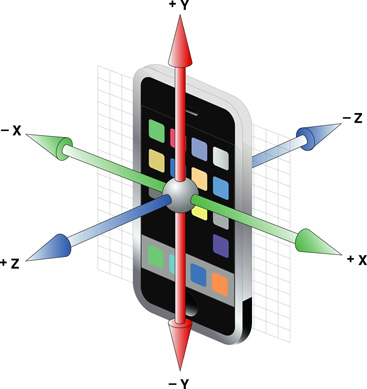
\includegraphics[width=0.38\linewidth]{xyz}
    \caption{Disposición de los ejes de un dispositivo Android.}
    \label{fig:xyz}
\end{figure}    

\begin{minipage}{\linewidth}
\begin{lstlisting}[caption={Código que se ejecuta cada vez que se registra un cambio en el sensor que calcula la orientacion.}, label={lst:orientacionL}]
    //Escuchamos los cambios en el sensor y hacemos los calculos
    public void onSensorChanged(SensorEvent event) {
        //Valor del sensor en grados
        double radians = event.values[0]; 
        //Convertimos en radianes
        radians = Math.toRadians(radians);
        //Obtenemos la ultima posicion registrada del GPS
        LatLng lastPosition = getCurrentPos();
        if (auxpos != null) { //Si la posicion no es nula
            //Le preguntamos a objeto de la clase ``Navigation'' las instalaciones 
            //que se encuentran en esa direccion
            allResultsSites = navULL.whatCanSee(lastPosition, radians);
        }
        //Si obtenemos al menos un resultado
        if (allResultsSites != null) {
            //Obtenemos la instalacion mas cercana, el indice 0 corresponde a la mas cercana
            nearSiteResult = allResultsSites.get(0);
            ... //Mostramos su informacion por pantalla para que usuario sepa que la instalacion  
                //que se encuentra apuntando
            if(allResultsSites.size() > 2) {
                ... //Si obtenemos mas de una instalacion mostramos al usuario el boton
                    //que indica el numero de instalaciones que se encuentran en la misma
                    //direccion 
            }
        } else { ... }
    } 
\end{lstlisting}
\end{minipage}

\subsection{Modelos encargados de la navegación}

A continuación, pasaremos a explicar la clases que intervienen en el proceso de reconocimiento de las instalaciones de la ULL que se encuentran delante del dispositvo móvil.

\subsubsection{ULLSite.java}

Cada instalacion de ULL se obtiene de una base de datos en formato JSON. Una instalacion se representa con un objeto de la clase ``ULLSite''. Ésta contiene toda su información y los atributos y funciones necesarias para poder trabajar con ella (véase Listado \ref{lst:ULLSite}). El objeto en formato JSON a partir de cual se creara el objeto de cada instalación se puede ver en la Figura \ref{fig:ull-site}.

\lstinputlisting[language=java, caption={Fichero \texttt{BaseActivity.java}. Código que se encarga de configurar la vista del Navigation Drawer.}, label={lst:ULLSite},]{listings/models/ULLSite.java}

\begin{figure}[h] 
    \centering
    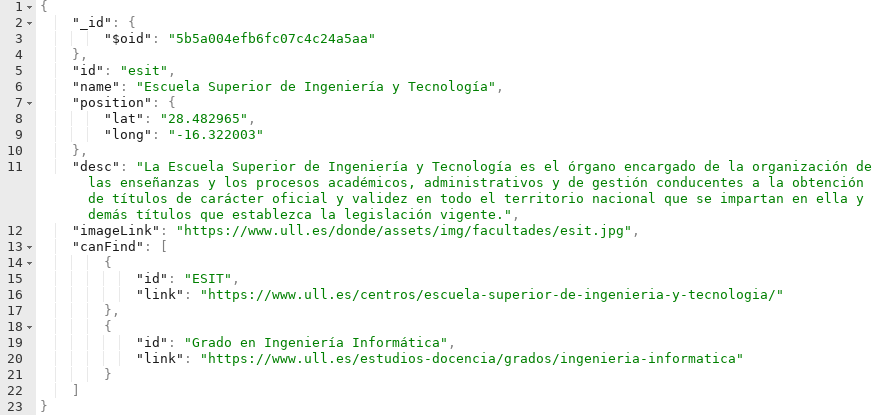
\includegraphics[width=150mm,scale=1]{ull-site}
    \caption{Ejemplo de una instalación de la ULL en la base de datos.}
    \label{fig:ull-site}
\end{figure}

En la clase ULLSite.java encontramos los atributos necesarios para guardar toda la información de cada instalación. Los tres útlimos atributos:  ``distToSite'' corresponde a la distancia entre el dispositivo y la instalacion, ``dirToSite'' corresponde con la dirección en la que se encuentra la instalación en el mundo con respecto al dispositivo y ``coneValue'' reprenta un rango de amplitud  con respecto a ``dirToSite'' a partir del cual se considerará que el dispositivo esta apuntando a la instalación, el valor de esta variable vendra dado por la distancia del dispositivo a la instalación. Estas variables junto con el objeto ``point'' de la clase ``Vector2D'', que contiene la ubicación en un plano coordenadas de dos dimensiones (``x'' e ``y''), permitirá realizar los cálculos para identificar si el dispositivo se encuentra en frente de esta instalación o no. En la Figura \ref{fig:dirSite} se explican los valores de estas variables.

\begin{figure}[h] 
    \centering
    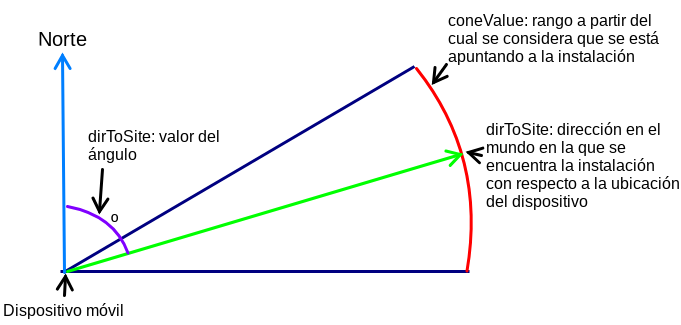
\includegraphics[width=160mm,scale=1]{calculateDirSite}
    \caption{Explicación de las variables ``coneValue'' y ``dirToSite''.}
    \label{fig:dirSite}
\end{figure}

  
\subsubsection{Navigation.java}

La clase ``Navigation'' es la clase principal encargada de  ejecutar todos métodos y realizar todos los calculos que permiten identificar las instalaciones. A partir de los datos obtenidos de los sensores y de las ubicaciones de las instalaciones permite identificar el centro más cercano que se encuentra en la dirección del dispositivo y también el resto de centros en esta misma dirección. En el Listado \ref{lst:NavigationResumen} podemos ver las variables y métodos de la clase.

\bigskip

\lstinputlisting[language=java, caption={Fichero \texttt{Navigation.java}. Clase ``Navigation'' que contiene las variables y métodos para los cálculos de las instalaciones.}, label={lst:NavigationResumen},]{listings/NavigationResumen.java}

A continuación se explicara de forma detallada la implementación de los métodos principales de esta clase.

En Listado \ref{lst:calculateCone} encontramos el método que calcula el tamaño de la variable ``coneValue'' de una instalación. El valor de ésta se calcula de modo que cuanto más cerca se encuentre el dispositivo de una instalación, mayor sea el rango con el que poder decidir si se encuentra delante de ella o no y, por el contrario, que este valor sea menor cuando se encuentre lejos de la instalación.
\bigskip
\begin{lstlisting}[caption={Código para calcular el \textit{coneValue} de identificación de cada instalación.}, label={lst:calculateCone}]
    public double calculateCone(double dist) {
        //Si es una instalacion "cercana" del dispositivo
        if (dist <= NEAR_VALUE){
            //Calculamos el valor del coneValue restandole al valor maximo las distancia a la instalacion por la constante SCALE_CONE_NEAR que permite que esta se escale gradualmente.
            return MAX_CONE_GRADS_NEAR - dist * SCALE_CONE_NEAR;
        }else { //Si es "lejana"
            //Calculamos el valor del coneValue restandole al valor maximo las distancia a la instalacion por la constante SCALE_CONE_FAR que permite que esta se escale gradualmente en instalaciones lejanas.
            double auxCone = MAX_CONE_GRADS_FAR - dist * SCALE_CONE_FAR;
            if (auxCone < MIN_CONE_GRADS) {
                return MIN_CONE_GRADS;
            } else {
                return auxCone;
            }
        }
    }
\end{lstlisting}

El cálculo del ángulo formado pos dos puntos geográficos lo realizamos con el método ``Vector2D.getAngleRad(Vector2D v2)'', como podemos ver en el Listado \ref{lst:angle}.

\begin{lstlisting}[caption={Metodo que cálcula el ángulo formado por dos puntos.}, label={lst:angle}]
    public double getAngleRad(Vector2D v2) {
        double dx = v2.getX() - getX(); //Caculamos las distancias en el eje x e y
        double dy = v2.getY() - getY();
        double radian = Math.atan2(dy, dx); //Relizamos la arcotangente para calcular el angulo
        return radian; //Devolvemos el resultado
    }
\end{lstlisting}

A este valor calculado, hay que aplicarle unas transformaciones para que se ajuste a la orientacion del norte magnético como el inicio de la rotación (norte magnético = 0º), para ello, el método ``Navigation.recalculeAng(double angleRad)'' se encarga de la correcta reorientación (véase Listado \ref{lst:reca}). 

\begin{lstlisting}[caption={Método que recalcula en ángulo para orientarlo en función del norte magnético.}, label={lst:reca}]
    private double recalculeAng(double angleRad) {
        double aux = rotateRad(angleRad); //Rota -pi/2
        aux = invertAng(aux);             //Invertimos el angulo 
        return aux;                       //Devolvemos el resultado
}   
\end{lstlisting}

El método ``whatCanSee'' \ref{lst:whatCanSee} es el metodo principal que se encargara, a partir de los datos de ubicación y direccion del dispositivo, de indentificar que instalaciones se encuentran en frente del dispositivo y cual es la más cercana. Para ello, en un primer paso, calculamos las distancias de las  instalaciones y las que se encuentran a una distancia mayor que ``maxDist'' y menor que ``minDist'' serán descartadas, para poder reducir el número de instalaciones a identificar. A continuación, para cada instalación anterior calculamos su dirección, posición y el valor del cono, con respecto a la ubicación del dispositivo. Si la instalacion se encuentra orientado dentro del cono que se forma en la dirección de la instalación, esta instalación se considerará como un posible resultado y se añadirá a la variable con una lista de estos resultados, ``result''. De los posibles resultados, la instalación más cercana al dispositivo será la instalación ante la que teoricamente se encuentra el dispositivo y guardará ésta el principio de esta lista.
 
\begin{lstlisting}[caption={Metodo principal que realiza el cálculo que permite reconocer las instalaciones en frente al dispositivo móvil.}, label={lst:whatCanSee}]
    //Metodo principal que se encarga identificar las instalaciones en frente del dispositivo
    //Recibe la posicion y orientacion actual del dispositivo
    //Devuelve la lista de instalaciones en esa direccion indicando cual es la mas cercana 
    public ArrayList<ULLSite> whatCanSee(LatLng currentPosAux, double actualDir) {
        currentPos.set(actualPos.longitude, actualPos.latitude); //Posicion actual del dispositivo
        currentDir = actualDir;  //Orientacion del dispositivo
        int id = -1;  //indice de la instalacion mas cercana en frente del dispositivo
        double nearSiteDist = maxDist; //distancia maxima valida para identificar un instalacion
        //Array a devolver con las instalaciones encontradas
        ArrayList<ULLSite> result = new ArrayList<>(); 
        //Calculamos todos los sitios que se encuentran entre maxDist y minDist
        for (int i = 0; i < allSites.size(); i++) {
            double distToSite = getDistanceBetween(currentPos, allSites.get(i).getPoint());
            if ((distToSite < maxDist) && (distToSite > minDist)) {
                destSites.add(allSites.get(i));
            }
        }
        //Para cada los sitio dentro del rango anterior 
        for (int i = 0; i < destSites.size(); i++) {  
            //Calculamos la direccion, distancia y valor del cono de cada instalacion a partir 
            //de la actual ubicacion del dispositivo
            double dirToSite = recalculeAng(currentPos.getAngleRad(destSites.get(i).getPoint()));
            double distToSite = getDistanceBetween(currentPos, destSites.get(i).getPoint());
            double coneValue = calculateCone(distToSite);
            //Comprobamos si el dispositivo esta orientado hacia dentro del cono que se forma en  
            //la direccion de la instalacion
            if (isInCone(dirToSite, coneValue)) { 
                //Guardamos los valores calculados anteriormente en el objeto ULLSite del array
                destSites.get(i).setConeValue(coneValue); 
                destSites.get(i).setDirToSite(dirToSite); 
                destSites.get(i).setDistToSite(distToSite); 
                result.add(destSites.get(i)); //Guardamos este sitio como resultado
                if (nearSiteDist > distToSite) { //Comprobamos si es el sitio mas cercano
                    nearSiteDist = distToSite; //Si lo es, actualizamos la distancia mas cercana
                    id = i;                    //Guardamos el indice de la instalacion mas cercana
                }
            }
        }
        if (id != -1) {                        //Si hemos encontrado alguna instalacion
            result.add(0, destSites.get(id));  //La instalacion mas cercana la guadamos la primera
            return result;                     //Devolvemos las instalaciones                   
        } else
            return null;                        //Si no encontramos ninguna instalacion
    }
\end{lstlisting}



 

\subsection{Obtención de la información}

Como hemos comentado anteriormente, toda la información perteneciente a las instalaciones de la ULL estarán en una base de datos. Además, para comunicarse con ésta, se dispone de un servidor que atienda a las peticiones de la aplicación, se conecte con esta base de datos y  envié la información. Más adelante, en el capítulo \ref{chap:BackEnd}, explicaremos detalladamente como funciona esta base de datos y servidor. Por ahora nos centraremos en explicar como realizamos la conexión con el servidor y el tipo de respuesta que obtenemos.

Para poder realizar una petición al servidor utilizaremos la clase ``GetData''. Que formaliza la petición con la url que le pasemos como parámetro a la función ``doInBackground'' y devuelve un string con la respuesta del servidor. En el Listado Listado \ref{lst:getData} podemos ver como funciona esta función. 

\lstinputlisting[language=java, caption={Fichero \texttt{GetData.java}, Código encargado de la conexión con el servidor y manejar la respuesta.}, label={lst:getData},]{listings/models/GetData.java} 

En el Listado \ref{lst:getSitesFromDB} encontramos el método ejecutado en la clase ``ARNavigation'' para realizar la conexión con el servidor para obtener la respuesta de la base de datos con todas las instalaciones de ULL. Posteriormente, se creará una instancia de la clase ``Navigation'' con todas las instalaciones de la base de datos en formato JSON. Este objeto lo denominaremos con el nombre de ``navULL'' y será el objeto encargado de identificar las instalaciones y trabajar con ellas.

\bigskip
\bigskip
\bigskip
\bigskip

\begin{lstlisting}[caption={Método que conecta con el servidor y recibe la respuesta con todas las instalaciones de la base de datos.},  label={lst:getSitesFromDB}]
    private void getSitesFromDB() {
        try{
            GetData getSites = new GetData();
            String sites = getSites.execute("https://server-ull-ar.herokuapp.com/api/ull-sites").get();
            JSONArray array = new JSONArray(sites);
            //Creamos una instancia del la clase "Navigation" con todas las instalaciones
            //Este es el objeto encargado de encontrar las instalaciones
            navULL = new Navigation(array); 
        } catch (JSONException e) {...}
}
\end{lstlisting}

Los últimos datos que se necesitan para trabajar con en el objeto ``navULL'' son los valores de ``maxRadius'' y ``minRadius'', los cuales el usuario puede editar en la ventana de \textit{Configuración} y que podemos acceder desde cualquier activity gracias a las ``Shared Preferences". Las Shared Preferences son un conjunto de datos accesible desde cualquier activity de la aplicación y que se utiliza para guardar los ajustes del usuario. En el método ``getRadius()'' del Listado \ref{lst:shared} vemos como se accede a estos datos.

\begin{lstlisting}[language=java, caption={Fichero \texttt{ARNavigation.java}, código que se encarga de guardar los valores de ``maxDist'' y ``minDist'' del objeto ``navULL''},  label={lst:shared}]
    private void getRadius() {
        try {
            //Obtenemos los valores configurables "maxRadius" y "minRadius" en la ventana de "Configuracion"
            settingsPref = PreferenceManager.getDefaultSharedPreferences(getContext());
            String auxMaxRadius = settingsPref.getString("maxRadius", "null");
            String auxMinRadius = settingsPref.getString("minRadius", "null");
            navULL.setMaxDist(Integer.parseInt(auxMaxRadius)); //Guardamos el valor "maxRadius"
            navULL.setMinDist(Integer.parseInt(auxMinRadius)); //Guardamos el valor "minRadius"
        }catch (Exception e){ ... }
    }
\end{lstlisting}


\subsection{Visualización}

El activity ``ARNavigation'' será el encargado de mostrar la técnica de realidad aumentada por geolozación en la pantalla de dispositivo móvil. Este activity hereda de la clase ``ARActivity'' perteneciente al  SDK de Kudan para Android Studio. Este SDK permite el reconocimiento de objetos e imágenes a trávez de la camara del dispositivo y queda como recurso para una futura ampliación de la funcionalidad de la aplicación. El uso principal de esta clase es el acceso que otorga a cámara del dispositivo como vista principal del activity. Es decir, permite visualizar en la ventana lo que se esta observando con la cámara.

Para poder hacer uso del SDK de Kudan tenemos que descargar el SDK y configurar la ``ARAPIkey'' específica para nuestro proyecto. Ambos los podemos encontrar en la página oficial de Kudan \cite{URL::kudan}. 

El archivo que contiene el SDK descargado, llamado \texttt{KudaAR.aar}, tenemos que pegarlo en la carpeta \textit{/app/libs/} de nuestro proyecto. A continuación tenemos de añadir la siguiente linea de código a las dependencias del fichero \texttt{build.gradle} de la aplicación:

\begin{lstlisting}
    implementation(name: 'KudanAR', ext: 'aar')
\end{lstlisting}

La configuración de la clave de la API de Kudan se realizará con el código del Listado \ref{lst:arapi}.

\begin{lstlisting}[caption={Fichero \texttt{ARNavigation.java}, código para configurar la API de Kudan.},  label={lst:arapi}]
    protected void onCreate(Bundle savedInstanceState) { //Cuando se inicie el activity
        ...
        ARAPIKey key = ARAPIKey.getInstance(); 
        key.setAPIKey("ARAPIKey..."); //ARAPIKey, clave generada por Kudan para el proyecto
    }
\end{lstlisting}
 
El fichero \texttt{aractivity.xml} (véase Listado \ref{lst:aractivity.xml}) contiene el layout con la información a mostrar al usuario cuando esté delante de una instalación. Este layout muestra al usuario en la parte superior de la ventana, el nombre de instalación ante la que se encuentra y un botón que le permite acceder a una ventana con la ficha de información de la instalación. Además incorpora un botón en la parte inferior que le indica el número de instalaciones adicionales que encuentran en la misma dirección. Al pulsar este botón se despliega una ventana con una lista de estas instalaciones.

\lstinputlisting[stringstyle=\color{purple},language=XML, caption={Fichero \texttt{aractivity.xml}, layout del activity ``ARNavigation''.}, label={lst:aractivity.xml},]{listings/aractivity.xml}

Los elementos del layout se mostrarán o ocultarán en función de si el usuarios se  encuentra en frente de una instalación o no, como podemos ver en el Listado \ref{lst:orientacionL}, se muestra como y cuando se alterna la información del layout.

Por último tenemos que configurar el funcionamiento de los botones ``moreInfoButton'' y ``moreSitesButton'' (véase Listado \ref{lst:infobutton}), que mostrarán una ventana con la ficha de información de la instalación y una ventana con una lista que contiene las instalaciones que tambien se encuentran la dirección a la que estamos orientados respectivamente. 

\begin{lstlisting}[caption={Fichero \texttt{ARNavigation.java}, código para manejar los eventos de los botones.},  label={lst:infobutton}]
    public void onClick(View v) {
        if(v.getId() == moreSitesButton.getId()){ //Si coincide
            //Se inicializa el activity que muestra la lista de los sitios adicionales
            Intent intent = new Intent(this, SitesListActivity.class);
            ArrayList aux = new ArrayList(moreResultsSites.subList(1, moreResultsSites.size()-1));
            SitesArray sitesArray = new SitesArray(aux);
            //Se le pasa una la lista con los sitios a mostrar
            intent.putExtra("sitesToShow", sitesArray);
            startActivity(intent); //Iniciamos el activity
        }
        if(v.getId() == moreInfoButton.getId()){ //Si coincide
            //Se inicializa el activity que muestra la descripcion de la instalacion
            Intent intent = new Intent(getApplicationContext(), SiteDescriptionActivity.class);
            ULLSiteSerializable actualULLSite = new ULLSiteSerializable(nearSiteResult);
            //Se le pasa como "extra" el objeto que contiene la informacion del sitio
            intent.putExtra("actualULLSite", actualULLSite);
            startActivity(intent); //Iniciamos el activity
        }
    }
\end{lstlisting}


\section{Fragmentos}

Los fragmentos \cite{URL::fragment} actuan como una sección modular de un activity que tiene su ciclo de vida propio, es decir, recibe sus propios eventos de entrada y que se pueden agregar o quitar mientras el activity se esté ejecutando. Se han utilizados estos fragmentos para mostrar el contenido de ciertas ventanas de la aplicación. La principal ventaja que nos aportan los fragmentos, es la facilidad que se tiene para intercambiar fragmentos dentro de un mismo activity y la mejora de rendimiento que se obtiene con respecto a creación de un activity para cada ventana que queramos en nuestra aplicación.

\subsection{MapsFragment}
       
Este fragmento contiene el mapa generado por la API de Google Maps. Para poder utilizar esta API, tenemos que acceder a la consola de desarrolladores de Google \cite{URL::consoleGoogle}. En ella tenemos que crear un proyecto con el nombre de nuestra aplicación, para después habilitar la API de ``Maps SDK for Android". Una vez habilitada se nos otorgará una clave que tendremos que en el fichero \texttt{app/res/values/google\_maps\_api.xml} (véase Listado \ref{lst:apiMaps}).

\begin{lstlisting}[stringstyle=\color{purple},language=XML,caption={Fichero \texttt{google\_maps\_api.xml}.},  label={lst:apiMaps}]
<resources>
    <string name="google_maps_key" templateMergeStrategy="preserve" translatable="false">API_Maps</string>
</resources>
\end{lstlisting}
 
A su vez, debemos añadir la siguiente linea a las dependencias de fichero \texttt{build.gradle} de la aplicación:
 
\begin{lstlisting}
    implementation 'com.google.android.gms:play-services-maps:15.0.1'
\end{lstlisting}

Con esto ya podremos utilizar la API de Google Maps en nuestra aplicación. Ahora nos toca configurar el fragmento de que contendrá la vista de Google Maps. 

Crearemos un fragmento en Android Studio con el nombre de \textit{MapsFragment}. Se generará un fichero llamado \texttt{MapsFragment.java} y un layout asociado, \texttt{fragment\_maps.xml}.

La clase ``MapsFragment'' (véase Listado \ref{lst:mapsF}) se encargará de: obtener la ubicación, dibujar en el mapa los marcadores las instalaciones de ULL, la ubicación del dispositivo y, si se activa en los ajustes, las dos circunferencias, cuyo centro es la ubicacion del dispositivo y que representaran un rango de busqueda de las instalaciones. Este rango funcionará a modo de que solo aparezcan las instalaciones que se encuentran en el espacio entre las dos circunferencias. En esta clase se harán uso de los métodos que ya vimos para obtener la ubicación GPS, las instalaciones de la base de datos y los datos necesarios guardados en las Shared Preferences.   

\bigskip

\lstinputlisting[caption={Fichero \texttt{MapsFragment.java}, métodos principales.}, label={lst:mapsF},]{listings/MapsFragment.java}

El fichero \texttt{fragment\_maps.xml}(véase Listado \ref{lst:mapsL}) contiene la vista del mapa de Google Maps en el cual se dibujaran los marcadores y los circulos que hemos comentado. Además incorpora un botón con el nombre de ``AR Mode'' que lanzará la ventana de \textit{Navegación en modo AR} que contiene el modo de realidad aumentada.

\lstinputlisting[stringstyle=\color{purple},language=XML,caption={Fichero \texttt{fragment\_maps.xml}.}, label={lst:mapsL},]{listings/fragment_maps.xml}
    

\subsection{HomeFragment}

El fragmento ``HomeFragment'' es la primera vista que encontramos cuando iniciamos sesión con éxito en la aplicación. Para el diseño de este fragmento se decidio por utilizar el modelo de ``RecyclerView'' \cite{URL::recycler}. Este modelo nos permite la visualización de listas de elementos de una forma más flexible, permitiendo configurar el contenido de cada elemento mediante el uso de adaptadores. Un adaptador permite crear las vistas de cada item de la lista a partir del contenido de las variables de cada uno de ellos. Además, cada adaptador gestiona los eventos cuando un item es seleccionado.

El contenido de cada item vendrá dada por la clase ``ItemHome'' (véase Listado \ref{lst:itemhom}). Los atributos de esta clase serán: una imagen, un nombre, una variable si indica si es o no un enlace externo del navegador y la url del enlace.

\begin{lstlisting}[caption={Fichero \texttt{ItemHome.java}.},  label={lst:itemhom}]
public class ItemHome {
    private String name;        //Nombre
    private String image;       //Ruta de la imagen
    private boolean isWebLink;  //Si es true es un enlace web externo
    private String link;        //Ruta del enlace
    //Constructor con los parametros
    public ItemHome(String name, String image, boolean isWebLink, String link){
        this.name = name;
        ...
    }
    ... //Get() y Set() metodos de los atributos
}
\end{lstlisting}

Con una lista de estos items, nuestro adaptor construirá el layout de cada item y luego se incorporarán a la vista de RecyclerView. La clase encargada de este procedimiento se llamará ``ItemHomeAdapter'' y hereda del adaptador ``RecyclerView.Adapter'' (véase Fichero \ref{lst:adapterItem}). Los atributos de esta clase son: una lista de los items, el layout con el diseño de cada item y un objeto ``OnItemClickListener'' que manejará los eventos de cada item. Dentro de esta clase, tendremos una clase ``ViewHolder'' que hereda de ``RecyclerView.ViewHolder'' y se encargará de enlazar el contenido de cada item con su layout. El layout con la vista de cada item lo encontraremos en el fichero \texttt{adapter\_item\_home.xml} (véase Fichero \ref{lst:itemView}). Este layout contendrá la imagen del item en la parte superior y el nombre inferior.
     
    
\lstinputlisting[stringstyle=\color{purple},language=XML,caption={Fichero \texttt{adapter\_home\_item.xml}.}, label={lst:itemView},]{listings/adapter_home_item.xml}

\bigskip


\begin{lstlisting}[caption={Fichero \texttt{ItemHomeAdapter.java}, clase que contruye las vistas de los items.},  label={lst:adapterItem}]
public class ItemHomeAdapter extends RecyclerView.Adapter<ItemHomeAdapter.ViewHolder> {
    private List<ItemHome> items;
    private int layout;
    private OnItemClickListener itemClickListener;
    public ItemHomeAdapter(List<ItemHome> items, int layout, OnItemClickListener listener){
        ... //Asignamos a los atributos con sus respectivos valores
    }
    //El parametro @ViewGroup parent contendra la vista de todos los items
    public ViewHolder onCreateViewHolder(@NonNull ViewGroup parent, int viewType) {
        View v = LayoutInflater.from(parent.getContext()).inflate(layout, parent, false);
        ViewHolder vh = new ViewHolder(v);     //Objeto ViewHolder  
        return vh;                             //Devolvemos la vista    
    }
    //Enlazamos cada item con su objeto ViewHolder
    public void onBindViewHolder(@NonNull ViewHolder holder, int position) {
        holder.bind(items.get(position), itemClickListener);
    }
    //Clase que hereda de RecyclerView.ViewHolder que sera la vista de cada item
    public static class ViewHolder extends RecyclerView.ViewHolder { 
        public TextView itemName;     
        public ImageView itemImage;   
        ...
        public ViewHolder(View itemView) { //Constructor con el layout
            ... //Enlazamos los objetos con el layout
            this.itemName= itemView.findViewById(R.id.textView_home_item);     
            this.itemImage = itemView.findViewById(R.id.imageView_home_item);
        }
        //Asignamos a cada vista el contenido de su item correspondiente 
        public void bind(final ItemHome itemHome, final OnItemClickListener listener){
            this.itemName.setText(itemHome.getName()); //Asignamos el texto
            ... //Asingamos la ruta de la imagen
            itemView.setOnClickListener(new View.OnClickListener() { ... });//Listener del item
    }
}
\end{lstlisting}

La clase ``HomeFragment''(véase Listado \ref{lst:homeF}) se encargará de instanciar los objetos de la clase ``ItemHome'' y el adaptador, ``ItemHomeAdapter'', para que se situén correctamente en la vista que contiene el RecyclerView (véase Listado \ref{lst:homeL}). 

\lstinputlisting[stringstyle=\color{purple},language=XML,caption={Fichero \texttt{fragment\_home.xml}.}, label={lst:homeL},]{listings/fragment_home.xml}
  

\lstinputlisting[caption={Fichero \texttt{HomeFragment.java}.}, label={lst:homeF},]{listings/HomeFragment.java}


\subsection{AboutFragment}

El fragmeto ``AboutFragment'' se encargar de mostar la ventana de la aplicación con la información general de la aplicación. Este consta simplemente de un fichero \texttt{Fragment.java} que muestra el layout que contiene esta información (véase Listado \ref{lst:aboutL}).

\lstinputlisting[stringstyle=\color{purple},language=XML,caption={Fichero \texttt{fragment\_about.xml}.}, label={lst:aboutL},]{listings/fragment_about.xml}


\section{Menú}

El menú de la aplicación constituye el elemento principal por el que el usuario navegará por la misma. Por ello se optado por incorporar un menú lateral deslizante llamado \textit{Navigation Drawer}. Este ha sido implementado por Google y lo encontramos en sus principales aplicaciones como ``Gmail'' y ``Google Play''. Un menú Navigation Drawer es un layout que incorpora dentro del mismo la vista de otras ventanas que se encuentren formato de fragmentos  y facilita que el cambio entre los fragmentos sea fluido y rápido. Este menú (véase Figura \ref{fig:menuApp}) se desplegará pulsando en la esquina superior izquierda de la aplicación.
   
El fichero \texttt{navigation\_draw.xml} contiene la vista del Navigation Draw. Aqui contamos con layout para el contenido principal a mostrar en la aplicación, la barra superior de la aplicación la que ira el nombre de \textit{ULL-AR}, un ``FrameLayout'' en el que ira el fragmento actual a mostrar y un ``NavigationView'' que será la vista del menú que un inicio estará sin desplegar.

\lstinputlisting[stringstyle=\color{purple},language=XML, caption={Fichero \texttt{navigation\_draw.xml}. Layout del Navigation Drawer.}, label={code:navigation_draw.xml},]{listings/navigation_draw.xml}

En cuanto al menú del Navigation Drawer, tenemos una cabecera (véase Listado \ref{code:header_navigation_drawer.xml}) con una imagen de la ULL y el debajo el nombre del usuario. Debajo de la cabecera tenemos las opciones del menú que vienen dadas por el fichero \texttt{nav\_options.xml} (véase Listado \ref{lst:nav_options.xml}). Cada uno de los items de opciones tiene un id, icono asociado y nombre.


\lstinputlisting[stringstyle=\color{purple},language=XML, caption={Fichero \texttt{header\_navigation\_drawer.xml}. Cabecera del Navigation Drawer.}, label={code:header_navigation_drawer.xml},]{listings/header_navigation_drawer.xml}
   

\lstinputlisting[stringstyle=\color{purple},language=XML, caption={Fichero \texttt{nav\_options.xml}. Opciones del menu Navigation Drawer.}, label={lst:nav_options.xml},]{listings/nav_options.xml}

Para la implementación del menú se utilizado una clase heredable llamada \texttt{BaseActivity.java} la cual incorpora la vista del Navigation Drawer, gestionará las opciones de el menú, cambiará los fragmentos y lanzará los activities principales de ULL-AR. 


\lstinputlisting[language=java, caption={Fichero \texttt{BaseActivity.java}. Código que se encarga de configurar la vista del Navigation Drawer.}, label={BaseActivity.java},]{listings/BaseActivity.java}



        
\section{Instalaciones de la ULL}

En la base de datos se encuentran con la gran mayoría de las instalaciones de la ULL. Recordamos que todas estas instalaciones constan de su nombre, posicion, una breve descripción del mismo y una lista de enlaces a los servicios, grados, departamentos, etc. Toda esta información es accesible por el usuario, mediante la ventana de \textit{Todas las instalaciones} (véase Figura \ref{fig:allSitesApp}). Esta ventana permite al usuario buscar la facultad, edificio o centro, que se encuentre en la base de datos, para posteriormente permitirle acceder a la ficha de información de la instalación (véase Figura \ref{fig:siteInfoApp}). En esta ficha se encontrará el resto de la información con respecto a es instalación.

En la ventana de \textit{Todas las instalaciones}  aparecerá una lista con todas las instalaciones con: su imagen a la izquierda y su nombre y descripción a la derecha. Para la creación de los items de la lista se opto por el uso de adaptadores al igual que en el fragmento ``HomeFragment'', pero sin la necesidad de una vista RecyclerView. La clase encargada de representar las instalaciones es ``SiteAdapter'', la cual hereda de la clase ``BaseAdapter'' de Android y, además, implementa la interfaz ``Filterable'' que permite aplicar, de forma dinámica, un filtro de busqueda sobre la lista de las instalaciones (véase Listado \ref{lst:SiteAdapter.java}). 



\lstinputlisting[language=java, caption={Fichero \texttt{SiteAdapter.java}.}, label={lst:SiteAdapter.java},]{listings/adapters/SiteAdapter.java}

Para la lista con los objetos a representar, se ha utilizado la clase ``ULLSiteSerializable'' que es una copia la clase  ``ULLSite'' (véase Listado \ref{lst:ULLSite}) pero que implementa la interfaz ``Serializable'' para permitir el paso de este objeto entre activities. 

El activity ``SiteListActivity'' se encargará de instanciar el adaptador con la lista de instalaciones que reciba del anterior activity y, dispondrá en la barra superior de la aplicación la barra de busqueda. Esta barra de busqueda le dirá al adaptador el filtro que tiene aplicar cada vez que se escriba en ella o cuando el usuario le de al botón de buscar. Cuando una instalación de la lista sea seleccionada se lanzará el activity ``SiteDescriptionActivity'' y se le pasará el objeto que contiene la instalación seleccionada.

\lstinputlisting[language=java, caption={Fichero \texttt{SiteListActivity.java}.}, label={lst:SiteListActivity.java},]{listings/SitesListActivity.java}
    

La activity ``SiteDescriptionActivity'' muestra toda la información de la instalación contenida en el objeto ``ULLSiteSerializable'' que envió activity que lo ejecuto o lanzo a este. Es una ventana que dispondrá: de la imagen de la instalación junto con botón en la parte inferior que abrirá la ruta de la aplicación en Google Maps, el nombre de la instalación, su descripción y una serie de enlaces relacionados con esta. Cuando uno de los enlaces es seleccionado, se abrirá el navegador externo del dispositivo móvil.

 
\lstinputlisting[language=java, caption={Fichero \texttt{SiteListActivity.java}.}, label={lst:SiteListActivity.java},]{listings/SiteDescriptionActivity.java}
 
    
\section{Preferencias del usuario}

Necitamos un lugar donde el usuario pudiera editar los ajustes de la aplicación. Se ha utilizado la clase ``PrefenceActivity'' que ofrece Android para diseñar la ventana. El fichero \texttt{pref\_nav\_setting.xml} (véase Listado \ref{lst:pref_nav_setting.xml} contendrá la lista con los ajustes. Estos ajustes nos permitiran decidir si queremos encontrar las instalaciones, en el mapa o en el modo realidad aumentada, dentros de dos circunferencias y la dimensiones en metros de ambos radios. 

\lstinputlisting[language=XML, caption={Fichero \texttt{pref\_nav\_setting.xml}.}, label={lst:pref_nav_setting.xml},]{listings/pref_nav_settings.xml}

Esta ventana de preferencias que ofrece Android nos permite trabajar con las Shared Preferences para guardar los ajustes y poder acceder a ellos en otras ventanas de la aplicación. En la clase ``SettingsULLActivity'' se inserta la vista con nuestras preferencias.

\lstinputlisting[float,floatplacement=H,language=java, caption={Fichero \texttt{SettingsULLActivity.java}.}, label={lst:SettingsULLActivity.java},]{listings/SettingsULLActivity.java}

% ---------------------------------------------------
%
% Trabajo de Fin de Grado. 
% Author: Alejandro Hernández Padrón. 
% Capítulo: La aplicación ULL-AR. 
% Fichero: Cap5_StartApplication.tex
%
% ----------------------------------------------------
%

\chapter{Conclusiones y futuras líneas de Trabajo} \label{chap:Conclusiones} 

En este capítulo se presentarán las conclusiones a las que se ha llegado tras realizar este TFG y se discutirán posibles líneas de trabajo futuras.

\section{Conclusiones}
 
Actualmente la realidad aumentada está invadiendo nuestras vidas, cada día se descubren nuevas muestras de lo que esta tecnología es capaz. La gran mayoría de sus futuras aplicaciones se encuentran aún en desarrollo debido a lo reciente y compleja que es esta tecnología. La RA se encontrará integrada en múltiples ámbitos tanto como profesionales dados sus aplicaciones en medicina e ingeniería, como en el de la enseñanza permitiendo a los estudiantes mejorar e incentivar el proceso de aprendizaje. 

En cuanto a la implementación y desarrollo de aplicaciones de RA, se encuentran limitadas al avance en el desarrollo de los SDK de RA que ofrecen empresas como Google, Apple o Vuforia, que cada día van ofreciendo más funcionalidades y mejor rendimiento pero que todavía tienen un amplio margen de mejora en función de lo que se espera de esta tecnología. Uno de los principales inconvenientes que se encuentra a la hora de desarrollar una aplicación de RA es elegir un SDK de RA que se adapte tanto a los requisitos como al presupuesto, ya que aunque la mayoría de los proveedores de estos SDK tienen versiones gratis para desarrolladores, a la hora de querer integrar esta tecnología en una aplicación,  la mayor parte de sus funcionalidades más interesantes para el reconocimiento de objetos en la nube, se encuentran con unos precios mensuales fuera del alcance de muchas empresas y desarrolladores.

En cuanto de la integración de un SDK de RA en Android Studio, se han encontrado con diversos problemas que dificultan trabajar con la RA en este IDE debido a que la mayoría de las empresas de RA que se encargan de desarrollar una versión de sus SDK para Android Studio, dejan de lado muchas funcionalidades y no ofrecen la documentación suficiente para instalar y empezar a trabajar con el SDK. En caso de querer realizar una aplicación de realidad aumentada de cierta calidad se recomienda el uso de plataformas de desarrollo 3D como Unity.



\section{Conclusions}

Nowadays, augmented reality is invading our lives, every day new samples of what this technology is capable of are being discovered. The great majority of its future applications are still under development due to the recent and complex nature of this technology. AR will be integrated in multiple fields, both as professionals given its applications in medicine and engineering, as well as in teaching, allowing students to improve and encourage the learning process. 

As for the implementation and development of AR applications, they are limited to the advance in the development of AR SDKs offered by companies such as Google, Apple or Vuforia, which every day are offering more functionality and better performance but still have a wide margin for improvement depending on what is expected of this technology. One of the main drawbacks when developing an AR application is to choose an AR SDK that fits both requirements and budget, since although most of the providers of these SDK have free versions for developers, when trying to integrate this technology into an application, most of its most interesting features for the recognition of objects in the cloud, are with monthly prices beyond the reach of many companies and developers.

As for the integration of an AR SDK in Android Studio, they have encountered several problems that make it difficult to work with AR in this IDE because most of the AR companies that are responsible for developing a version of their SDK for Android Studio, leave aside many features and do not offer enough documentation to install and start working with the SDK. If you want to make an augmented reality application of a certain quality is recommended the use of 3D development platforms such as Unity.

% \section{Líneas de trabajo futuras}

% En un futuro se podría ampliar la funcionalidad de la aplicación permitiendo a los usuarios no solo llegar a una instalación, si no moverse dentro de ellas para llegar a una clase, un laboratorio, el despacho de un profesor, etc. Sería de gran ayuda el uso de la tecnología de los ``beacons'' \cite{URL::beacon} para ubicar al dispositivo móvil dentro de una instalación.

% A su vez se podría implementar un algoritmo más preciso para la identificación de las instalaciones, ya que en las instalaciones de gran superficie el algoritmo utilizado no es el más optimo debido a que para el cálculo solo se tiene en cuenta un punto geográfico que encuentra en el centro de cada instalación. Lo ideal sería tener un área generada con los puntos geográficos de cada instalación e identificarlas cuando el usuario enfoque a esa área.




% El principal inconveniente con el que se encuentra la RA en el ambito profesional y de la enseñanza que los dispositivos  con suficiente capacidad de cómputo y que a su vez sean un medio hábil y práctico para su visualización, como pueden ser las Google Glass no se encuentran al alcance de cualquiera debido a su



\chapter{Presupuesto} \label{chap:RAEntornosUniversitarios} 

En este capítulo se expondrán las estimaciones de recursos necesarios para
desarrollar y publicar el proyecto.

El desglose del presupuesto de la aplicación se puede contabilizar de la siguiente manera:

\begin{itemize}
    \item En caso de que se desee publicar la aplicación en la Google Play Store, se necesita poseer de una cuenta de desarrolladores de Google. Para ello se necesitará disponer de una cuenta de Google a una de desarrolladores, se han de seguir los pasos en la web \cite{URL::googleplayconsole}, en la que pedirán un abono único de 25 dólares.  
    \item En cuanto a coste del servidor, Heroku ofrece distintos planes para la gestión de este.  En Heroku los ``dynos'' son las unidades que proveen capacidad de cómputo. El pago mensual en Heroku dependerá de la cantidad y la potencia de los dynos que se tengan contratados. Las cuotas por dyno que ofrece Heroku son:
    \begin{itemize}
        \item Free: 0 dólares al mes. 
        \item Hobby: 7 dólares por dyno al mes.
        \item Standard 1x: 25 dólares por dyno al mes.
        \item Standard 2x: 50 dólares por dyno al mes.
        \item Perfomance M: 250 dólares por dyno al mes.
        \item Perfomance L: 500 dólares por dyno al mes.
    \end{itemize}
    
    Los planes Free y Hobby no constan de mucha potencia y tienen limitados el número de procesos que pueden responder a las peticiones, son recomendadas para uso personal y de pequeñas aplicaciones. El resto de los planes ofrecen número de procesos ilimitados y permite la escalabilidad horizontal en el caso de que la aplicación lo requiera.

    Para los requisitos de la aplicación se necesitaría contratar  un dyno del plan Standard 1x. El coste mensual de este plan sería de 300 dólares al año.
    En caso de que el dyno contratado no sea capaz de soportar el tráfico de la aplicación se podría cambiar de plan o agregar otro dyno Standard 1x. 

    \item La base de datos se encuentra situada en la plataforma de mLab. Esta plataforma en función del número de GB que se necesiten para la base de datos ofrece los siguientes planes:
    \begin{itemize}
        \item Sandbox: 0.5 GB gratis. 
        \item Shared Cluster: 15 dólares al mes por GB.
        \item Dedicated Cluster: a partir de 180 dólares al mes por 40 GB. 
    \end{itemize} 

    El plan de Sandbox se ajusta a los requisitos de la base de datos de la aplicación, por lo que no tendría coste. 
    
    \item La información referente a cada instalación sería recomendable obtenerla de primera mano del personal encargado de cada instalación para asegurar que la información este completa y correcta. Esto supondría un costo de 300 o 400 euros para gastos de transporte e investigación.
    \item Desarrollador de la aplicación. dudas XXX.
    \item Sería recomendable el mantenimiento de la aplicación. Se ofrece un programador en Android con conocimientos en Node.js que se haría cargo de las incidencias que pudieran, del mantenimiento del servidor y de actualizar la información de la base de datos. Este programador trabajaría a jornada completa por  1500 euros al mes, lo que supone  un costo anual de 18000 euros.  
\end{itemize}  


 
  

 
\addcontentsline{toc}{chapter}{Bibliografía}
% \bibliographystyle{plain}
\bibliographystyle{ieeetr}
  % \bibliographystyle{bmc_article} 
\renewcommand{\bibname}{Bibliografía}   %  Para que no aparezca Índice de figuras
\bibliography{bibliografia}

%%%%%%%%%%%%%%%%%%%%%%%%%%%%%%%%%%%%%%%%%%%%%%%%%%%%%%%%%%%%%%%%%%%%%%%%%%%%%%%
 
\end{document}
